\documentclass{legrand}
\usepackage{thesis_98_packages}

%-------------------------------------------------------------------------------
%	SETTING UP SOME VARIABLES :D
%-------------------------------------------------------------------------------
\def\mytitle{Analysis and implementation of an algorithm to validate Knowledge Graphs using Big data techniques} % Title of the project
\def\subtitle{From a Rustacean's perspective} % Subtitle of the project
\def\centre{Escuela de Ingeniería Informática} % The name of the center you're sitting at
\def\reviewer{Jose Emilio Labra Gayo} % reviewer of the project
\def\author{Ángel Iglesias Préstamo} % Your name.. 
\def\date{\today} % Today's date 
%-------------------------------------------------------------------------------
%-------------------------------------------------------------------------------

\begin{document}

\hypersetup{
    pdftitle={\mytitle},
    pdfauthor={\author}
}

\pagenumbering{roman}

% custom commands for use in the paper
% creating some commands for reuse later on :D
\newcommand{\myfont}[1]{\ensuremath{\mathcal{#1}}}

\newcommand{\VertSet}{\myfont{V}}
\newcommand{\NodeSet}{\myfont{N}}
\newcommand{\EdgeSet}{\myfont{E}}
\newcommand{\LabelSet}{\myfont{L}}
\newcommand{\PLabelSet}{\myfont{T}}
\newcommand{\MsgSet}{\myfont{M}}
\newcommand{\None}{\myfont{None}}

\newcommand{\triple}[3]{\ensuremath{\langle #1,#2,#3 \rangle}}
\newcommand{\quadruple}[4]{\ensuremath{\langle #1,#2,#3,#4\rangle}}
\newcommand{\ItemSet}{\myfont{Q}}
\newcommand{\PropSet}{\myfont{P}}
\newcommand{\EntitySet}{\myfont{E}}
\newcommand{\ValueSet}{\myfont{V}}
\newcommand{\DataValueSet}{\myfont{D}}
\newcommand{\StmtSet}{\rho}
\newcommand{\FinSet}[1]{\ensuremath{FinSet(#1)}}
\newcommand{\Graph}{\myfont{G}}

\newcommand{\hrefc}[3][blue]{\href{#2}{\color{#1}{#3}}}%
\newcommand{\elemento}[2]{\ensuremath{\hrefc[violet]{http://www.wikidata.org/entity/#2}{#1}}}
\newcommand{\propiedad}[2]{\ensuremath{\hrefc[blue]{http://www.wikidata.org/entity/#2}{#1}}}
\newcommand{\alanTuring}{\elemento{alanTuring}{Q7251}}
\newcommand{\wilmslow}{\elemento{wilmslow}{Q2011497}}
\newcommand{\town}{\elemento{town}{Q3957}}
\newcommand{\government}{\elemento{government}{Q220798}}
\newcommand{\warringtonLodge}{\elemento{warringtonLodge}{Q20895942}}
\newcommand{\bombe}{\elemento{bombe}{Q480476}}
\newcommand{\unitedKingdom}{\elemento{unitedKingdom}{Q145}}
\newcommand{\computer}{\elemento{computer}{Q11742076}}
\newcommand{\dateOfBirth}{\propiedad{dateOfBirth}{P569}}
\newcommand{\placeOfBirth}{\propiedad{placeOfBirth}{P19}}
\newcommand{\country}{\propiedad{country}{P27}}
\newcommand{\employer}{\propiedad{employer}{P108}}
\newcommand{\discoverer}{\propiedad{discoverer}{P61}}
\newcommand{\dateOfDeath}{\propiedad{dateOfDeath}{P570}}
\newcommand{\placeOfDeath}{\propiedad{placeOfDeath}{P20}}
\newcommand{\timeStart}{\propiedad{timeStart}{P580}}
\newcommand{\timeEnd}{\propiedad{timeEnd}{P582}}
\newcommand{\manufacturer}{\propiedad{manufacturer}{P176}}
\newcommand{\Human}{\elemento{Human}{Q5}}
\newcommand{\instanceOf}{\propiedad{instanceOf}{P31}}

\newcommand{\fb}[1]{\dofb#1}
\newcommand{\dofb}[1]{\textbf{#1}\nobreak\hspace{0pt}}

\newcommand{\mi}[1]{\ensuremath{\mathit{#1}}}

\newcommand{\emptyGraph}{\ensuremath{\emptyset}}
\newcommand{\EmptyGraph}{\ensuremath{\emptyset}}
\newcommand{\addTriple}{\ensuremath{\rtimes}}
\newcommand{\unionGraphs}{\ensuremath{\cup}}
\newcommand\neighs[2]{\ensuremath{neighs(#1,#2)}}
\newcommand\nodes[1]{\ensuremath{nodes(#1)}}
\newcommand{\node}{\mi{n}}
\newcommand{\lbl}{\mi{l}}
\newcommand{\g}{\mi{g}}
\newcommand{\vertex}{\mi{v}}
\newcommand{\msg}{\mi{msg}}
\newcommand{\msgs}{\mi{msgs}}
\newcommand{\labels}{\mi{labels}}
\newcommand{\TripleConstraint}{\mi{TripleConstraint}}
\newcommand{\ShapeReference}{\mi{ShapeReference}}
\newcommand{\ShapeAnd}{\mi{ShapeAnd}}
\newcommand{\ShapeOr}{\mi{ShapeOr}}
\newcommand{\Cardinality}{\mi{Cardinality}}

% Algorithmic definitions
\SetKwProg{Def}{def}{$\,$:}{}
\SetKwProg{Defn}{def}{~$=$}{}
\SetKw{defn}{def}
\newcommand{\DefInline}[2]{\defn #1 = #2}
\SetKwProg{DefnCustom}{\defn}{}{}
\SetKw{Let}{let}
\SetKwInput{KwIn}{Input}
\SetKwFor{ForEach}{foreach}{}{}
\SetKw{Or}{or}
\SetKw{And}{and}
\SetKwIF{If}{ElseIf}{Else}{if}{then}{else if}{else}{endif}
\SetKw{Match}{match}
\SetKw{MyIf}{if}
\SetKw{MyThen}{then}
\SetKw{MyElse}{else}
\SetKw{Case}{case}
\SetKwBlock{Let}{let}{in}
\SetKw{In}{in}
\SetKw{MapTo}{\ensuremath{\;\;\Rightarrow\;\;}}
\SetKwBlock{Block}{}{}
\newcommand{\assign}{\ensuremath{~\mathtt{:=}~}}
\newcommand{\algocomment}[1]{\text{//$\,$#1}}

\newcommand{\blockskip}{\smallskip}
\newcommand{\done}{\ensuremath{\mathit{done}}}

% [algorithm spacing:]
\def\algorithmsize{small}
\def\algorithmheadersize{\algorithmsize}
\renewcommand\AlCapFnt{\normalfont\bfseries\small}
\setlength{\textfloatsep}{1.0ex}
\setlength{\floatsep}{1.0ex}

% Statuses
\newcommand{\Ok}{\ensuremath{Ok}}
\newcommand{\Failed}{\ensuremath{Failed}}
\newcommand{\WaitingFor}[3]{\ensuremath{WaitingFor}(#1,#2,#3)}
\newcommand{\Pending}{\ensuremath{Pending}}
\newcommand{\PendingLs}{\ensuremath{Pending}(ls)}
\newcommand{\Undefined}{\ensuremath{Undefined}}

\newcommand{\Validate}{\ensuremath{Validate}}
\newcommand{\Checked}[2]{\ensuremath{Checked(#1,#2)}}
\newcommand{\WaitFor}[1]{\ensuremath{WaitFor(#1)}}
\newcommand{\status}[2]{\ensuremath{#1(#2)}}
\newcommand{\msgSent}[3]{\ensuremath{#1,#2\rightsquigarrow{}#3}}
\newcommand{\checkLocal}[2]{\ensuremath{checkLocal(#1,#2)}}
\newcommand{\checkLocalOpen}[2]{\ensuremath{checkLocalOpen(#1,#2)}}

\newcommand{\neighbors}[3]{\ensuremath{neighbors}(#1,#2,#3)}
\newcommand{\fracEmpty}[2]{\genfrac{}{}{0pt}{0}{#1}{#2}}
\newcommand{\vProg}{vProg}
\newcommand{\tripleConstraints}[1]{tripleConstraints(#1)}
\newcommand{\rbe}[1]{\ensuremath{rbe(#1)}}
\newcommand{\combine}[2]{\ensuremath{combine(#1,#2)}}

\chapterimage{img/misc/heading_main.pdf} % Chapter heading image
\begingroup
\thispagestyle{empty}
\begin{tikzpicture}[remember picture,overlay]
    \coordinate [below=10cm] (midpoint) at (current page.north);
    \node at (current page.north west)
    {\begin{tikzpicture}[remember picture,overlay]
            \node[anchor=north west,inner sep=0pt] at (0,0) {
\includegraphics[width=\paperwidth]{img/cover_bg}}; % Background image
            \draw[anchor=north] (midpoint) node [fill=blueUniovi!30!white,fill opacity=0.6,text opacity=1,inner sep=1cm, text width=21cm, minimum width=\paperwidth]
            {\Huge\centering\bfseries\sffamily\parbox[c][][t]{\paperwidth}
            {\centering\mytitle\\[15pt] % Book title
            {\Large\subtitle}\\[20pt] % Subtitle
            {\huge\author}\\[1pt] % Author's name
            {\large Supervised by \textit{\reviewer}} % Reviewer's name
            }};
        \end{tikzpicture}};
\end{tikzpicture}
\vfill
\endgroup

% include the abstract, written in a separate file called thesis_02_abstract.tex
\setcounter{page}{0}
\newenvironment{abstract}%
{\cleardoublepage\null\vfill\section*{\abstractname}}%
{\vfill\null}
\begin{abstract}
    The necessity of processing large amounts of data is getting increased with time. Not only we do need to process high volumes of sequential information, but more complex structures such as graphs. As an example of that, one of the sources we can retrieve data from is Wikidata, the central storage for the structured data of Wikimedia projects: including Wikipedia. The shape of the documents to be processed from Wikidata tends to be heterogeneous: the structure of a human node may vary from the one of a mountain. More in more, it could be helpful to generate subsets out of a dump for us to work only with concrete nodes.

    Not only that but, the last tendencies in \textit{data integration} show that the data is not only stored in a single place but distributed among different sources. This is the case of biological data where several different databases are used to store the information, including \texttt{Uniprot} and \texttt{PubChem}. The data is stored in different formats, and it is not always easy to integrate it. However, through \textit{subsets} we can create a common ground for the data to be processed. This is, we can create a subset of the data that is common to all the sources, and then process it.
\end{abstract}

\noindent \textbf{Keywords} --- \textit{Knowledge Graphs, RDF, Linked Data, RDF Validation, Shape Expressions, Subsets, MapReduce, Pregel, Algorithms, Wikibase, Apache Spark, Scala, Rust, DuckDB.}
\phantom{~}

\vfill

\begingroup

\section*{Acknowledgements}

\noindent Put your acknowledgments here.

\endgroup

\vfill
\phantom{~}

\vfill

\begin{flushright}
    {\em
        Data is a precious thing\\[0.25\baselineskip]
        and will last longer than the systems themselves\\[1.5\baselineskip]
        --Tim Berners-Lee
    }
\end{flushright}

\bigskip

\vfill

% Create a table of contents - not mandatory
\pdfbookmark{\contentsname}{toc}
\tableofcontents

% Create a list of figures
\listoffigures

% Create a list of tables
\listoftables


\chapter{Introduction}
% and we establish the numeration back to the normal one 
\setcounter{page}{0} % reset numbering to 1, 2, 3...
\pagenumbering{arabic}
\label{chapter:intro}
\epigraph{\textit{We cannot solve problems with the kind of thinking we employed when we came up with them.}}{-- \textup{Albert Einstein}}

In the following paragraphs, we are covering the motivation, contributions and structure of this document. This means, after reading it, you are building the big picture; a general idea of the motivations to develop this project, the goal we are looking forward to achieving and the shape of the document itself.

\section{Motivation}

A famous mathematical problem from the past is \textbf{The Seven Bridges of Königsberg}. The foundations of \textit{graph theory} were set by Leonhard Euler's negative resolution\footnote{The \textbf{negative resolution} system consists of applying the resolution rule where one of the clauses being a negative literal.} to the problem in 1736.

The city of Königsberg in Prussia (now Kaliningrad, Russia) was built on both banks of the \textit{Pregel River} and featured two sizable islands, Kneiphof and Lomse, which were linked to the two mainland sections of the city by seven bridges. The challenge was creating a route through the city that would cross each of those bridges just once. What Euler proved was that this problem has no solution.

\begin{figure}[ht]
    \begin{subfigure}{.3\textwidth}
        \centering
        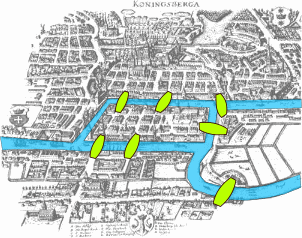
\includegraphics[width=.7\linewidth]{img/4-1_konigsberg_bridges.png}
        \caption{The seven bridges' exact positioning is shown on Königsberg's map from Euler's time, highlighting the Pregel River in blue}
    \end{subfigure}%
    \hspace*{0.5em}
    \begin{subfigure}{.3\textwidth}
        \centering
        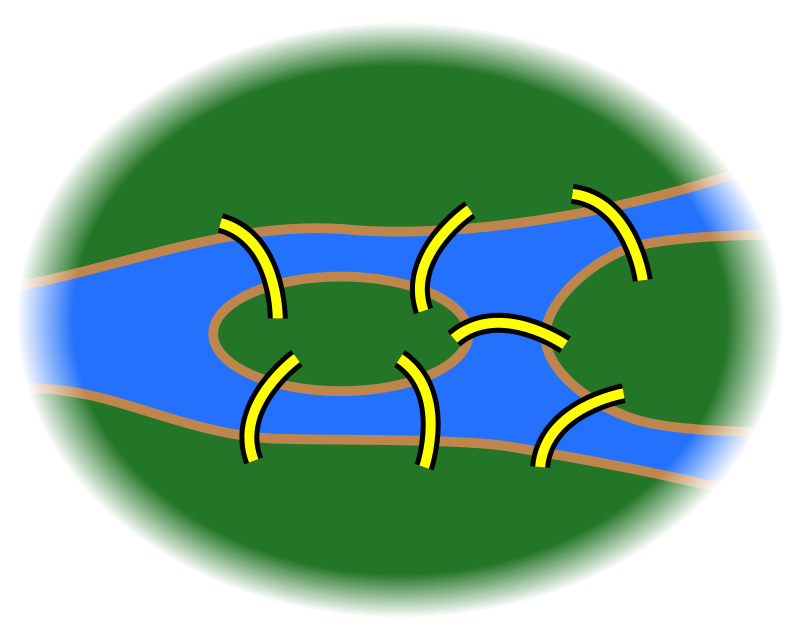
\includegraphics[width=.7\linewidth]{img/4-2_konigsberg_abstract.png}
        \caption{Diagram illustrating The Seven Bridges of Königsberg's puzzle. Take note of how our level of abstraction has increased}
    \end{subfigure}%
    \hspace*{0.5em}
    \begin{subfigure}{.3\textwidth}
        \centering
        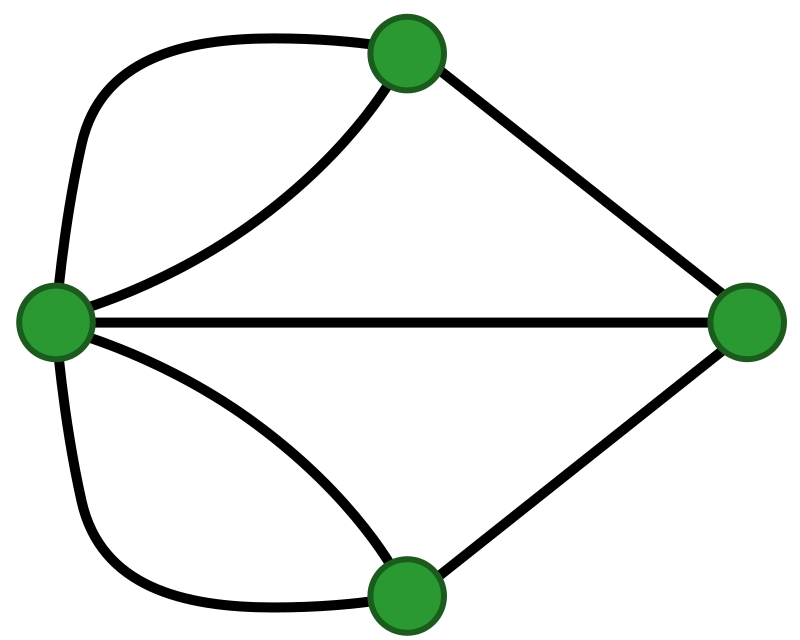
\includegraphics[width=.7\linewidth]{img/4-3_konigsberg_graph.png}
        \caption{Abstract graph corresponding to the bridges of Königsberg, where edges are de bridges and nodes are the sectors of the city}
    \end{subfigure}%
    \caption[Creating the equivalent graph of the problem of The Seven Bridges of Königsberg]{Creating the equivalent graph of the problem of The Seven Bridges of Königsberg\footnotemark}
\end{figure}
\footnotetext{\url{https://en.wikipedia.org/wiki/Seven_Bridges_of_Konigsberg}}

\subsection{Eueler's analysis}

In modern terms, Euler observed that the degree of the nodes; that is, the number of vertices connected to a particular element, determines the possibility of a walk around a graph, traversing each edge precisely once. According to Euler's theory, a connected graph with exactly zero or two nodes with odd degrees is a requirement for the walk around the entire network. This is because we can only cross each bridge once, therefore each traversal of a section of the city requires an even number of edges to be crossed. For each entrance on a mainland, we must enter through one bridge and exit through another. It turns out that this condition is also sufficient. We also know that if there are nodes with odd degrees, then any path will begin at one of them and end at the other. A path like this is currently known as the Eulerian path and is named after the mathematician. Summing up, we have proved that there can be no Eulerian path in the graph that corresponds to Königsberg since it contains four nodes of odd degrees.

\section{Project Scope}

A growing number of devices are interconnected, these days. As a result, tons of data is being automatically stored. This way, processing that data becomes both a more challenging and important task. Simply stated, the amount of data we try to handle outruns our capacity to consume it. Big data, a new area of software development, where we quickly handle large volumes of heterogeneous information, offers a remedy for this.

Interoperability is a crucial subject we must deal with in big data applications since they not only need to scan huge volumes of inputs as quickly as possible but also because the information comes from a range of sources.

Knowledge graphs~\cite{https://doi.org/10.48550/arxiv.2110.11709} were popularized back in 2012 by Google~\cite{web:knowledge_graphs:google} as a tool to represent real-world data reflecting relationships between entities to understand those links better. After Google's introduction, others embraced this approach: ranging from proprietary to open databases. Being the content of the latter publicly available. Prominent companies -- including \textit{web search} (e.g., Bing~\cite{knowledge:graphs:usage:bing} and Google~\cite{web:knowledge_graphs:google}), \textit{commerce} (e.g., Airbnb~\cite{knowledge:graphs:usage:airbnb} and Amazon~\cite{knowledge:graphs:usage:amazon}), \textit{social networks} (e.g., Facebook~\cite{knowledge:graphs:usage:facebook} and LinkedIn~\cite{knowledge:graphs:usage:linkedin}) or \textit{finances} (e.g., Accenture~\cite{knowledge:graphs:usage:accenture} and Banca d'Italia~\cite{https://doi.org/10.48550/arxiv.2010.05172}) -- are using knowledge graphs to have a better understanding of their customers. Even though there exist several models associated with this technology, we are focusing on Wikibase graphs.

Summing up, this project focuses on the analysis and implementation of a system to validate Wikibase graphs -- a specific flavor of the so-called knowledge graphs -- using big data techniques. To put that into perspective, as of October 1, 2022, a compressed dump\footnote{A \textbf{dump} is a copy of the whole Wikibase raw data that can be downloaded from their system. This could also be understood as a snapshot of what was stored in the system at a certain moment} of Wikidata's database has a size of 109.04GB~\cite{wikidata:dumps}. Not only that, but the size of these dumps has exponentially increased with every release (see Figure \ref{fig:dumps}).

\begin{figure}[ht]
    \centering
    \includestandalone[width=0.4\textwidth]{diagrams/1-1_dumps}
    \caption[Plot showing the size of compressed dumps between 2014-22]{Size of compressed Wikidata dumps between 2014-2022~\cite{https://doi.org/10.48550/arxiv.2110.11709}}
    \label{fig:dumps}
\end{figure}

These enormous sizes make it difficult for users to easily examine and process the content of them, and they also raise the possibility that these technologies will become victims of their success. This condition is demonstrated in Scholia, an online application that uses Wikidata to describe data about academics and their works. The app includes appealing visualizations and comparisons that are based on requests through the Wikidata endpoint. Despite the project offering a wealth of intriguing data, timeouts caused by the massive volumes of information prevent access to the most intricate visualizations.

Creating subsets of the Knowledge Graphs for specific domains may be one solution to these problems. These subsets serve as snapshots of the data at certain points in time and can be used to enhance the performance of the apps that consume that data, making it easier to research the contents of Knowledge Graphs.

\label{section:objectives}
\section{Objectives}

\paragraph{Project's Goal 1}
\textit{Design and implementation of a system for validating huge dumps from Wikidata generating a subset out of it.} As we have stated during these introductory lines, the task of having to process enormous amounts of data is becoming increasingly relevant. The faster a system allows us to accomplish it, the better solution we will provide. We are not only interested in Wikidata dumps but also other Knowledge graphs. The more generic the solution is, the better.

\paragraph{Project's Goal 2}
\textit{Reproduce an experiment related to the analysis of the previously described algorithm.} For us to properly analyze the results emerging from the execution of the algorithm we have implemented, we have to create an ecosystem where we can obtain information related to memory consumption or execution time, to name a few. This way, we are willing to create a solution that is capable of being executed in commodity hardware.

\paragraph{Project's Goal 3}
\textit{Learn new technologies and Big data techniques.} As this is an academic project and one of the main objectives of a research project is finding innovative solutions to a certain problem: learning and exploring new possibilities is -- indeed -- one of this project's goals.

\section{Contributions}

Having the main objective and motivations introduced, let me highlight the key contributions of this project. Take note that the document is divided into several parts, one per each of the contributions listed below.

\begin{enumerate}
    \itemsep0.5em
    \item Research and documentation of the existing method for validating Wikibase Knowledge Graphs provided a schema that the graph's entities should conform to. The suggested solution is implemented in Scala and Apache Spark; yet, at the project's first meeting, several proposals for enhancing the real solution were presented. The original code was rewritten according to the aforementioned research, although the resulting solution was far from ideal. The process of exploring and refactoring the code is enumerated in the chapters to come.
    \item Presentation of a novel Rust and SQL-based Knowledge Graph subset generation architecture. The goal is to provide a solution that can run on any hardware efficiently. We are willing to explore the capabilities of Rust for enabling some performance gains regarding single-node computation. What's more, when comparing them to NoSQL, relational databases are on the rise. According to some early findings, the JSON dump is 10 times larger in size than the generated single database file. More on this will be discussed in the following chapters.
\end{enumerate}

\section{Structure of the document}

The shape of this document is as follows:

\begin{itemize}
    \itemsep0.25em
    \item[\textbf{Chapter ~\ref{chapter:related}.}] General description of the existing technologies related to knowledge graph validation. As well as the advantages and disadvantages of choosing some tools over others for implementing this project.
    \item[\textbf{Chapter ~\ref{chapter:theory}.}] Provides a theoretical background needed for a better understanding of the concepts explained in the following chapters.
    \item[\textbf{Chapter ~\ref{chapter:existing}.}] Description of the initial solution implemented by Labra, serving as the project's baseline.
    \item[\textbf{Chapter ~\ref{chapter:refactoring}.}] Description of the changes introduced to the original solution, as well as the reasons behind them.
    \item[\textbf{Chapter ~\ref{chapter:analysis}.}] Analysis of the new perspective introduced by the final solution. As well as the advantages and disadvantages of choosing some tools over others for implementing this project.
    \item[\textbf{Chapter ~\ref{chapter:wd2duckdb}.}] Description of the process followed to create the new solution based on Rust and DuckDB.
    \item[\textbf{Chapter ~\ref{chapter:pschema}.}] Explanation of the process followed to create the algorithm that validates the knowledge graphs.
    \item[\textbf{Chapter ~\ref{chapter:experiment}.}] Explanation of the process followed to analyze the concrete implementation of the algorithm that we used to validate the knowledge graphs.
    \item[\textbf{Chapter ~\ref{chapter:results}.}] Analysis of the results obtained from the previously described experiment.
    \item[\textbf{Chapter ~\ref{chapter:planning}.}] Summary of the process followed to create this final degree project, as well as some considerations regarding management and organization of resources.
    \item[\textbf{Chapter ~\ref{chapter:conclusions}.}] Summary of the general conclusions and future work.
\end{itemize}

\chapter{State of the art}
\label{chapter:related}
\epigraph{\textit{If I have seen further, it is by standing on the shoulders of giants.}}{-- \textup{Isaac Newton}}

Some work has already been done in the field of Knowledge Graph validation. In this section, we are exploring what other projects have achieved and their limitations.

\section{Big data processing and graphs}

Due to the need to handle massive graphs, Google proposed Pregel~\cite{10.1145/1807167.1807184} as a model for large-scale graph computing back in 2010. This idea of \textit{thinking like a vertex} led to the introduction of other systems such as GraphLab~\cite{10.14778/2212351.2212354}, PowerGraph~\cite{180251}, and GraphX~\cite{186216}. The latter is a framework that facilitates the implementation of parallel computing algorithms.

In the present day, alternative approaches have emerged, particularly when considering performance in single-node systems. Rust-based solutions like \texttt{pola-rs}\footnote{\url{https://www.pola.rs/}} have been developed to process large graphs on a single computer due to their highly optimized parallel execution capabilities. This brings up the question of whether it is feasible to process the Wikidata graph on a single computer.

\section{Knowledge graphs}

An introduction to the concept of a Knowledge Graph can be found in~\cite{10.1145/3447772}, which is also referenced in Labra's paper~\cite{https://doi.org/10.48550/arxiv.2110.11709}. In that article, the authors discuss the process of creating a knowledge graph, which bears similarities to the approach used in this document. They also emphasize the significance of data quality, which is the primary focus of this thesis. It is important to note that this document does not deal with the creation of a knowledge graph, but rather focuses on its validation. Furthermore, our work is particularly centered around processing Wikibase graphs, which were introduced in Labra's paper. Our description of Wikibase graphs draws inspiration from MARS (Multi-Attributed Relational Structures)~\cite{ijcai2017p165}, which presents a generalized concept of property graphs. Additionally, Labra's work defines MAPL (Multi-Attributed Predicate Logic) as a formalism of logic that can be applied to ontological reasoning.

\section{Knowledge Graph descriptions}

Several descriptions of knowledge graphs have been proposed, with many introduced in~\cite{https://doi.org/10.48550/arxiv.2110.11709}. Among them, the most relevant ones for this thesis are Property graphs, RDF graphs, and Wikibase graphs. In a Property graph, the nodes represent entities, and the edges represent properties. RDF graphs have entities as nodes and RDF triples as edges. Wikibase graphs, on the other hand, have entities as nodes and Wikibase statements as edges. It is worth noting that the Wikibase graph is a generalization of the RDF graph, and it is the one utilized in this thesis.

To create subsets, we will employ Shape Expressions, which were first introduced in 2014. While the W3C recommendation\footnote{\url{https://www.w3.org/TR/2017/REC-shacl-20170720/}} is SHACL (Shapes Constraint Language) since 2017, the Wikidata community has been using Shape Expressions~\cite{10.1007/978-3-030-21348-0_39}. This preference stems from the fact that Shape Expressions better adapt to describing data models compared to SHACL. A comparison between the two can be found in the following article~\cite{Labra2017}.

Improving the overall quality of knowledge graphs has been the focus of recent research~\cite{https://doi.org/10.48550/arxiv.2110.11709}.

\label{section:wd2sub}
\section{Knowledge Graph subsets}

As previously mentioned, the Wikidata knowledge graph is enormous, and it is not feasible to process it on a single computer using existing techniques. To address this challenge, we have developed a novel method to split the Wikidata graph into smaller subsets using Shape Expressions, as introduced in~\cite{https://doi.org/10.48550/arxiv.2110.11709}.

Although it is possible to create subsets of the RDF Knowledge Graph through SPARQL construct queries, there are limitations to this approach. Notably, the lack of support for recursion, which means representing cyclic data models is not possible. While proposals to extend SPARQL with recursion have been made~\cite{10.1007/978-3-319-25007-6_2}, such extensions are not widely supported by existing processors. Additionally, the verbosity of the solution, which requires the creation of scripts, makes it inconvenient for code development when generating subsets. In light of these limitations, we have developed a new method using Shape Expressions to create subsets of the Wikidata knowledge graph, as described in~\cite{https://doi.org/10.48550/arxiv.2110.11709}.

The creation of subsets in Knowledge graphs has gained attention, starting from the 12th International SWAT4HCLS Conference\footnote{\url{https://www.wikidata.org/wiki/Wikidata:WikiProject_Schemas/Subsetting}}. It has since been selected as a topic of interest in the Elixir Europe Biohackathon 2020\footnote{\url{hhttps://github.com/elixir-europe/BioHackathon-projects-2020/tree/master/projects/35}} and the SWAT4HCLS 2021 hackathon, which resulted in a preprint that collected various proposed approaches~\cite{10.37044/osf.io/wu9et}. The creation of knowledge graph subsets is of interest to the Wikidata community and the field of bioinformatics.

One of the proposed approaches is \texttt{WDumper}\footnote{\url{https://github.com/bennofs/wdumper}}, a tool that processes Wikidata dumps to generate subsets. It takes a JSON compressed dump and a JSON configuration file as inputs, applies filters according to the configuration, and produces an RDF compressed dump. The use of WDumper to generate Wikidata subsets is described in~\cite{wdumper}, where four subsets are created. This paper explores various use-case scenarios and highlights the strengths and weaknesses of this approach. However, one limitation of this approach is its lack of formalism compared to a ShEx-based method.

Another Python library, called WikiDataSets~\cite{boschin2019wikidatasets}, generates Wikidata subsets based on specific topics such as humans, countries, animal species, and films. However, this approach is less flexible compared to the ShEx-based method.

Lastly, \texttt{KGTK} (Knowledge Graph Toolkit)~\cite{ilievski2021kgtk} is a tool that facilitates working with knowledge graphs by introducing a common format called \texttt{KGTK} based on hypergraphs. This allows for the handling of various types of knowledge graphs using the same library. The concept of creating a higher-level abstraction for processing knowledge graphs, as demonstrated in this thesis (Chapter \ref{chapter:pschema}), aligns with the approach of \texttt{KGTK}. In line with \texttt{KGTK}, they have implemented a query language named Kypher~\cite{chalupsky2021creating}, which is an adapted version of \texttt{Cypher} specifically designed for \texttt{KGTK}. This enables the creation of subgraphs within the tool. They utilize SQLite queries to generate subgraphs, and this idea is also adopted in this thesis (see chapter~\ref{chapter:wd2duckdb}). However, we employ \texttt{DuckDB}\footnote{\url{https://duckdb.org/}} as the backend, following a similar approach to the one proposed in \texttt{wd2sql}\footnote{\url{https://github.com/p-e-w/wd2sql}}. The paper referenced above states that they can create subsets of the Wikidata knowledge graph on a laptop. This served as our main inspiration to develop a method for creating subsets on a single machine instead of employing a distributed approach.

Furthermore, during the development of this thesis, we came across a paper that compared several approaches for creating subsets of the Wikidata knowledge graph~\cite{wikidataTools}. In this paper, they evaluated and compared the performance of different approaches and tools. Their methodology for measuring performance and conducting experiments served as the primary inspiration for designing the experiments in chapter~\ref{chapter:experiment}.

\chapter{Theoretical Background}
\label{chapter:theory}
\epigraph{\textit{It doesn't matter how beautiful your theory is, it doesn't matter how smart you are. If it doesn't agree with the experiment, it's wrong.}}{-- \textup{Richard P. Feynman }}

In the following chapter, a description of the theoretical concepts needed for a proper understanding of this document is done. Ranging from \textit{knowledge graphs} to \textit{data-flow paradigms}, we are providing a firm foundation for the experiment to be conducted.

\section{Knowledge graphs}
\label{section:knowledgeGraph}

A knowledge graph uses a graph-structured data model to represent knowledge of some real-world domain. Where each node represents an entity -- a \textit{thing} from the actual world -- and the edges are the relationships between them. This type of graph is often assembled from a wide variety of sources, and as a result, can be highly diverse in terms of structure and granularity~\cite{DBLP:journals/corr/abs-2003-02320}. To address this issue, representations of \textit{schema}, \textit{identity} and \textit{context} are needed. While the former defines the high-level structure of the graph, \textit{identity} relates nodes that conform to the same real-world entity; finally, \textit{context} provides the environment for specific knowledge to be understood. Let me write a more formal definition of a knowledge graph:

\begin{definition}[Knowledge Graph]
    A knowledge graph is a graph-structured data model that captures knowledge in a specific domain, having nodes that represent entities and edges that represent relationships between their entities~\cite{https://doi.org/10.48550/arxiv.2110.11709}.
\end{definition}

Note that the definition above is as general as it gets. In this manner, a knowledge graph can be represented using different technologies. In the following sections, we will focus on the most representative examples of knowledge graphs: \textit{RDF graphs} and \textit{property graphs}. We will also discuss the \textit{Wikibase} data model, as it is the one used in the experiment to be conducted.

\subsection{RDF (Resource Description Framework) graphs}
\label{section:RDF}

Let me first introduce \textit{Resource Description Framework} (RDF) as it is the most simple and widely used technology for representing a knowledge graph model. RDF is a data interchange W3C standard for the web. It has been used as a method for the description and exchange of graph data\footnote{\url{https://en.wikipedia.org/wiki/Resource_Description_Framework}}, providing a variety of syntax notations and formats, with \texttt{Turtle} being the most adopted one. One of the main features of RDF is that it allows the combination of different data sources, even if the schemas differ from one another. What's more, it supports the evolution of schemas without requiring the data consumers to adapt to those changes.

RDF is a directed graph composed of triple statements; called \textit{semantic triples}, in the way of \textit{subject-predicate-object}. Where each element is identified by a URI. The \textit{subject} denotes the resource you want to make statements about, the \textit{predicate} denotes attributes of the resource and models relationships among the \textit{subject} and the \textit{object}, and the \textit{object} is the value of the attribute. As an example, we can represent that \textit{the genre of The Hunger Games is dystopian fiction} in RDF as the triple: a \textbf{subject} denoting \textit{The Hunger Games}, a \textbf{predicate} denoting \textit{is of genre}, and an \textbf{object} denoting \textit{dystopian fiction}. This representation can be seen in Figure \ref{fig:RDF}.

\begin{figure}[ht]
    \centering
    \includestandalone[width=0.8\textwidth]{diagrams/6-4_RDF}
    \caption{Directed knowledge graph generated out of a triple \textit{subject-predicate-object}}
    \label{fig:RDF}
\end{figure}

We have mentioned that the most common syntax notation for RDF is Turtle; however, one of the simplest is N-Triples. Each line of a \texttt{.nt} document is a single triple \textit{subject-predicate-object}, followed by a full stop, meaning the termination of the statement. All that together form a directed knowledge graph. Let's see an example of an RDF graph represented using N-Triples notation.

\begin{example}[RDF knowledge graph using N-Triples notation]
    \href{https://www.wikidata.org/entity/Q7251}{Alan Turing (Q7251)} \href{https://www.wikidata.org/entity/P19}{was born (P19)} in \href{https://www.wikidata.org/entity/Q20895942}{Warrington Lodge (Q20895942)} and \href{https://www.wikidataWShEx.org/entity/P108}{was employed (P108)} by the \href{https://www.wikidata.org/entity/Q220798}{Government of the United Kingdom (Q220798)} where he \href{https://www.wikidata.org/entity/P61}{discovered (P61)} the Enigma-deciphering machine \href{https://www.wikidata.org/entity/Q480476}{bombe (Q480476)}.
\end{example}

\begin{dumps}
    \inputminted{turtle}{code/listings/6-3_serialization.nt}
\end{dumps}

\subsection{Property graphs}

A property graph is a type of graph model where vertices and edges, namely nodes and relationships, are annotated with labels and properties. In this manner, property graphs excel at depicting connections between data and exposing data dependencies. When compared to other \textit{datastores}, such as relational databases, property graphs focus on how the recorded things relate, although descriptions of those items might be supplied via properties and attributes. In this sense, provided a real-world domain, expressing the relationships among data is just as crucial as the data itself.

With that in mind, it can be argued that there's no need for a new type of \textit{datastore} as relational databases are capable of storing those relationships through constraints. However expensive operations such as \texttt{JOIN} are required to navigate across those links. It turns out that relational databases handle relationships between data in a not-so-sophisticated manner. To tackle this issue, graph databases were created. In this model, relationships are stored natively alongside the nodes in a flexible format. Several commercial graph databases like Neo4j\footnote{\url{https://neo4j.com/}}, JanusGraph\footnote{\url{https://janusgraph.org/}} or Sparksee\footnote{\url{https://www.sparsity-technologies.com/\#sparksee}} were developed.

\begin{figure}[ht]
    \centering
    \includestandalone[width=0.8\textwidth]{diagrams/6-1_propertyGraph}
    \caption{Example of a property graph}
    \label{fig:propertyGraph}
\end{figure}

Note that figure \ref{fig:propertyGraph} is a simplified version of a property graph. This is because what we have tried here is to extend the example in figure \ref{fig:RDF} transforming the RDF graph into a property one.

\label{section:wikibase_graphs}
\subsection{Wikibase graphs}

Wikidata started back in 2012 as a support to Wikipedia. Rapidly becoming one of the biggest human knowledge bases, with remarkable organizations donating their data to it; as an example, Google migrated \textit{Freebase} -- its previous knowledge graph -- to Wikidata in 2017~\cite{10.1145/2872427.2874809}. As of October 9, 2022, Wikidata currently contains roughly 100 million items\footnote{\url{https://www.wikidata.org/wiki/Wikidata:Statistics}}. Internally, Wikidata's content is stored in a SQL database (MariaDB); however, this system is not ideal for querying or data analysis. With that in mind, and pursuing the integration of Wikibase within the semantic web ecosystem, the Wikimedia Foundation adopted BlazeGraph: an open-source triple store and graph database\footnote{\url{https://en.wikipedia.org/wiki/Blazegraph}}. This way, two data models coexist in Wikibase: a document-centric model based on MediaWiki, and an RDF-based one that can be used to perform SPARQL queries through the Query Service~\cite{https://doi.org/10.48550/arxiv.2110.11709}.

\begin{figure}[ht]
    \centering
    \includestandalone[width=0.5\textwidth]{diagrams/6-2_architectureWikibase}
    \caption[Simplified architecture of Wikibase]{Simplified architecture of Wikibase~\cite{https://doi.org/10.48550/arxiv.2110.11709}}
    \label{fig:architecture:wikibase}
\end{figure}

Informally speaking, the Wikibase data model is composed of \textit{entities} and \textit{statements} (about those entities). This way, an entity can be either an \textit{item} or a \textit{property}. Items are used to represent all the \textit{things} from human knowledge. Usually denoted by a \texttt{Q} followed by a sequence of digits; as an example, \href{https://www.wikidata.org/wiki/Q7251}{Q7251} represents Alan Turing in Wikidata. On the other hand, properties model a relationship between an item and a value, and are represented by a \texttt{P} followed by a sequence of numbers; as an example, \href{https://www.wikidata.org/wiki/Property:P31}{P31} is the property \textit{instance of} in Wikidata.

For values to be associated with properties, they must belong to some specific data type\footnote{\url{https://www.wikidata.org/wiki/Help:Data_type}}. Supported data types include URLs, time, quantities, and mathematical expressions; to name a few. Notice how more complex data types are also supported; those include \textit{properties} and \textit{items}, this way, relationships among entities are allowed.

Lastly, a statement is a piece of data about an item and is recorded on the page of the item itself. Putting it all together, the way Wikibase manages information is as follows: through a statement, we add information to a certain item using some property and its value. This can be seen in figure \ref{fig:wikibaseStatement}.

\begin{figure}[ht]
    \centering
    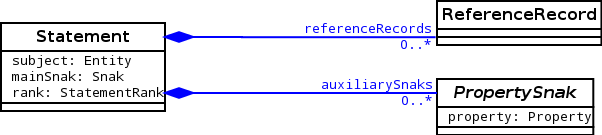
\includegraphics[width=.8\linewidth]{figures/diagrams/6-11_statement.png}
    \caption[Formal definition of a statement in Wikibase]{Formal definition of a statement in Wikibase\footnotemark}
    \label{fig:wikibaseStatement}
\end{figure}
\footnotetext{\url{https://www.mediawiki.org/wiki/Wikibase/DataModel\#Statements}}

The different components that appear in figure \ref{fig:wikibaseStatement} are as follows:

\begin{itemize}
    \itemsep0.25em
    \item \textbf{Subject}: the item to which the statement refers.
    \item \textbf{mainSnak}: the main \textit{property-value} pair for a certain entity.
    \item \textbf{Rank}: to tell if a certain \texttt{Statement} is \texttt{deprecated} or not.
    \item \textbf{referenceRecords}: a list of references that support the statement.
    \item \textbf{qualifierSnaks}: a list of qualifiers that modify the meaning of the statement.
\end{itemize}

This may seem to be a complex data model, but it is not. It is quite simple indeed. To illustrate this, we will use an example.

\begin{example}[Adding information to an entity in Wikidata\footnote{\url{https://www.wikidata.org/wiki/Help:Statements}}]
    \label{example:wikibaseGraph}
    To include information about the genre of \textit{The Hunger Games} in Wikidata, we would need to add a statement to the item itself: \href{https://www.wikidata.org/wiki/Q11679}{The Hunger Games (Q11679)}, using the property \href{https://www.wikidata.org/wiki/Property:P136}{genre (P136)}, we can then add the value \href{https://www.wikidata.org/wiki/Q15062348}{dystopian fiction (Q15062348)}. Notice how we are linking two entities (\textit{items}) of the Wikidata.
\end{example}

\begin{table}[ht]
    \centering
    \documentclass{standalone}
\usepackage[table,xcdraw]{xcolor}
\usepackage{varioref,multicol}
\usepackage{hyperref}  
\begin{document}
\begin{tabular}{|c|l|l|l|}
    \hline
    \rowcolor[HTML]{EFEFEF}
    \textbf{Language} & \multicolumn{1}{c|}{\cellcolor[HTML]{EFEFEF}\textbf{Item}}                              & \multicolumn{1}{c|}{\cellcolor[HTML]{EFEFEF}\textbf{Property}}                            & \multicolumn{1}{c|}{\cellcolor[HTML]{EFEFEF}\textbf{Value}}                             \\ \hline
    \textit{English}  & \multicolumn{1}{l|}{\href{https://www.wikidata.org/wiki/Q11678}{The Hunger Games}}      & \multicolumn{1}{l|}{\href{https://www.wikidata.org/wiki/Property:P136}{genre}}            & \multicolumn{1}{l|}{\href{https://www.wikidata.org/wiki/Q15062348}{dystopian fiction}}  \\ \hline
    \textit{Spanish}  & \multicolumn{1}{l|}{\href{https://www.wikidata.org/wiki/Q11678}{Los juegos del hambre}} & \multicolumn{1}{l|}{\href{https://www.wikidata.org/wiki/Property:P136}{género}}           & \multicolumn{1}{l|}{\href{https://www.wikidata.org/wiki/Q15062348}{ficción distópica}}  \\ \hline
    \textit{French}   & \multicolumn{1}{l|}{ \href{https://www.wikidata.org/wiki/Q11678}{Hunger Games}}         & \multicolumn{1}{l|}{\href{https://www.wikidata.org/wiki/Property:P136}{genre artistique}} & \multicolumn{1}{l|}{\href{https://www.wikidata.org/wiki/Q15062348}{fiction dystopique}} \\ \hline
    \textit{Wikidata} & \multicolumn{1}{c|}{\href{https://www.wikidata.org/wiki/Q11678}{Q11678}}                & \multicolumn{1}{c|}{\href{https://www.wikidata.org/wiki/Property:P136}{P136}}             & \multicolumn{1}{c|}{\href{https://www.wikidata.org/wiki/Q15062348}{Q15062348}}          \\ \cline{2-4}
\end{tabular}
\end{document}
    \caption[Including information about the genre of \textit{The Hunger Games}]{Including information about the genre of \textit{The Hunger Games}\footnotemark}
    \label{tab:language}
\end{table}
\footnotetext{\url{https://www.wikidata.org/wiki/Q11678}}

\subsubsection{Opaque URIs}
\label{section:opaqueURIs}

Recall that the main purpose of Wikidata is to store data about things that are described by pages in Wikipedia (in any language)\footnote{\url{https://www.mediawiki.org/wiki/Wikibase/DataModel}}. This means, \textit{things} should be represented in such a way that they don't depend on the natural language used; that is, language independence is required. In Wikidata, this is achieved through a linked data pattern called \textit{opaque URIs}. In general, a URI is defined as a unique sequence of characters that identifies the resources of the system\footnote{\url{https://en.wikipedia.org/wiki/Uniform_Resource_Identifier}}. Designing good URIs is the first step in linked data development.

The characters that appear in a URI tend to be related to the concept they represent, improving human readability. As an example, \texttt{https://example.com/España} could -- potentially -- be an identifier for the Spanish country. However, for those non-Spanish speakers, that identifier is meaningless. What's more, the use of non-ASCII characters may lead to problems in an internationalized system. Opposed to \textit{descriptive URIs}, \textit{opaque} ones are not intended to represent terms in a natural language~\cite{LabraGayo2015MultilingualLD}. An example of that is \url{https://www.wikidata.org/wiki/Q11679}, where item \texttt{Q11679} represents \textit{The Hunger Games} in Wikidata. However -- in some situations -- it is helpful for users to interact with human-readable names. In Wikidata, this is solved through \textit{labels}, which are language-dependent. Following the previous example, the label tagged to the entity \texttt{Q11679} is the actual title of the book: \textit{The Hunger Games}. Translations for several languages can also be provided. Notice table~\ref{tab:language} for an example of possible \textit{labels} for some \textit{opaque URIs}.

What we have seen so far is an overview of the Wikibase \textit{data model}; including: \textit{statements}, \textit{properties}, \textit{values} and the appropriate mechanism for identifying them (in a multilingual approach). The next step is to formally define what a Wikibase graph is.

\begin{definition}[Wikibase graphs]
    Given a mutually disjoint set of items $\mathcal{Q}$, a mutually disjoint set of properties $\mathcal{P}$, and a mutually disjoint set of values $\mathcal{V}$, a Wikibase graph is a quadruple $(\mathcal{Q}, \mathcal{P}, \mathcal{V}, \rho)$. Where $\rho \subseteq \mathcal{Q} \times \mathcal{P} \times \mathcal{V}$ is a set of statements.
\end{definition}

For a better understanding of this formal definition, let me explain it step-by-step. Any \textit{item} in $\mathcal{Q}$ can have information added to it using $\mathcal{Q}$ \textit{entities}, $\mathcal{P}$ \textit{properties}, or $\mathcal{V}$ \textit{data values}. Meaning that we can add a statement about a particular entity in $\mathcal{Q}$ using the aforementioned set of values. For us to provide extra information to a certain relationship, we may include it in the fourth entry of the quadruples in the $\rho$ set, see example \ref{example:knowledgeGraph} for more details. As an example, to establish the \href{https://www.wikidata.org/wiki/Property:P585}{point in time} at which \href{https://www.wikidata.org/wiki/Q937} {Albert Einstein} received the \href{https://www.wikidata.org/wiki/Q38104}{Nobel Prize in Physics}, we may annotate the \href{https://www.wikidata.org/wiki/Property:P166}{award received} property with the value 1921\footnote{\url{https://www.nobelprize.org/prizes/physics/1921/summary/}}. Those are called \textit{qualifiers}. For further clarification, let us model the Wikibase graph of a certain scenario.

\vspace*{-0.5em}

\begin{example}[Wikibase Knowledge Graph]
    \label{example:knowledgeGraph}
    We are willing to qualify that Alan Turing (23 June 1912 -- 7 June 1954) was employed by the government of the United Kingdom in the course of WWII. During that time he invented the computer for deciphering Enigma-machine-encrypted secret messages\footnote{\url{https://en.wikipedia.org/wiki/Bombe}}. Additional information about relevant places where he lived is also annotated.
\end{example}

\vspace*{-1.25em}

% Tikz File 'fig_03_wikibaseGraph.tex'
\documentclass{standalone}
\usepackage{tikz}
\usepackage{../mystyle}
\newcommand{\myfont}[1]{\ensuremath{\mathcal{#1}}}

\newcommand{\triple}[3]{\ensuremath{\langle #1,#2,#3 \rangle}}
\newcommand{\quadruple}[4]{\ensuremath{\langle #1,#2,#3,#4\rangle}}

\newcommand{\ItemSet}{\myfont{Q}}
\newcommand{\PropSet}{\myfont{P}}
\newcommand{\EntitySet}{\myfont{E}}
\newcommand{\ValueSet}{\myfont{V}}
\newcommand{\DataValueSet}{\myfont{D}}
\newcommand{\StmtSet}{\rho}
\newcommand{\FinSet}[1]{\ensuremath{FinSet(#1)}}

\newcommand{\hrefc}[3][blue]{\href{#2}{\color{#1}{#3}}}%

\newcommand{\elemento}[2]{\ensuremath{\hrefc[violet]{http://www.wikidata.org/entity/#2}{#1}}}
\newcommand{\propiedad}[2]{\ensuremath{\hrefc[blue]{http://www.wikidata.org/entity/#2}{#1}}}
\newcommand{\alanTuring}{\elemento{alanTuring}{Q7251}}
\newcommand{\wilmslow}{\elemento{wilmslow}{Q2011497}}
\newcommand{\town}{\elemento{town}{Q3957}}
\newcommand{\government}{\elemento{government}{Q220798}}
\newcommand{\warringtonLodge}{\elemento{warringtonLodge}{Q20895942}}
\newcommand{\bombe}{\elemento{bombe}{Q480476}}
\newcommand{\unitedKingdom}{\elemento{unitedKingdom}{Q145}}
\newcommand{\computer}{\elemento{computer}{Q11742076}}
\newcommand{\dateOfBirth}{\propiedad{dateOfBirth}{P569}}
\newcommand{\placeOfBirth}{\propiedad{placeOfBirth}{P19}}
\newcommand{\country}{\propiedad{country}{P27}}
\newcommand{\employer}{\propiedad{employer}{P108}}
\newcommand{\discoverer}{\propiedad{discoverer}{P61}}
\newcommand{\dateOfDeath}{\propiedad{dateOfDeath}{P570}}
\newcommand{\placeOfDeath}{\propiedad{placeOfDeath}{P20}}
\newcommand{\timeStart}{\propiedad{timeStart}{P580}}
\newcommand{\timeEnd}{\propiedad{timeEnd}{P582}}
\newcommand{\manufacturer}{\propiedad{manufacturer}{P176}}
\newcommand{\Human}{\elemento{Human}{Q5}}
\newcommand{\instanceOf}{\propiedad{instanceOf}{P31}}

\setlength{\tabcolsep}{1mm}
\renewcommand{\arraystretch}{1.5}
\usetikzlibrary{positioning,arrows}
\begin{document}
\begin{tikzpicture}[
        vertex/.style={
                rectangle,
                rounded corners,
                draw=black!60,
                fill=black!5,
                minimum width=15mm,
                minimum height=7.5mm,
                text centered,
                font=\footnotesize
            },
        predicate/.style = {font=\footnotesize\ttfamily},
        >= stealth',
        shorten >= 0.5pt
    ]
    \node[vertex,align=center] (alanTuring) at (-2, 0) {\alanTuring\\{\tiny \dateOfBirth  \hspace{1mm} \textit{23 June 1912}}\\{\tiny \dateOfDeath  \hspace{1mm} \textit{7 June 1954}}};
    \node[vertex] (human) at (-2, -2) {\Human};
    \node[vertex] (birth) at (2.75, 2.25) {\warringtonLodge};
    \node[vertex] (death) at (1, 4) {\wilmslow};
    \node[vertex] (employer) at (4, 0) {\government};
    \node[vertex] (country) at (7.25, 2.25) {\unitedKingdom};
    \node[vertex] (bombe) at (4, -2) {\bombe};
    \node[vertex] (machine) at (1, -3.25) {\computer};
    \node[vertex] (town) at (6, 4) {\town};

    \path[->] (alanTuring.north) edge[bend left] node[predicate,sloped,above] {\placeOfDeath} (death.west);
    \path[->] (alanTuring.north) edge[bend left] node[predicate,sloped,above] {\placeOfBirth} (birth.west);
    \path[->] (alanTuring.south) edge node[predicate,left] {\instanceOf} (human.north);
    \path[->] (alanTuring.east) edge node[label={[align=left,font=\tiny]above:\employer\\- \timeStart \hspace{1mm} \textit{1938}\\- \timeEnd \hspace{1mm} \textit{1945}}] {} (employer.west);
    \path[->] (birth.east) edge node[predicate,sloped,above] {\country} (country.west);
    \path[->] (bombe.south) edge[bend left] node[predicate,sloped,below] {\instanceOf} (machine);
    \path[->] (bombe.north) edge node[predicate,left] {\manufacturer} (employer.south);
    \path[->] (bombe) edge[bend left] node[predicate,sloped,above] {\discoverer} (alanTuring);
    \path[->] (bombe.east) edge[bend right] node[predicate,sloped,above] {\country} (country);
    \path[->] (death.east) edge node[predicate,above] {\instanceOf} (town.west);
    \path[->] (death) edge node[predicate,sloped,above] {\country} (country);
\end{tikzpicture}
\end{document}

\begin{figure}[H]
    \centering
    \includestandalone[width=0.9\textwidth]{diagrams/6-3_wikibaseGraph}
    \caption[Formal description and visualization of Turing's Wikibase graph]{Formal description and visualization of Turing's Wikibase graph}
\end{figure}

\subsubsection{Wikibase data serialization}
\label{section:wikibase:serialization}

The Wikibase data model supports two export formats, namely, JSON and RDF. Being the former the one employed by the JSON dumps and the latter follows semantic web and linked data principles. A fragment of both formats is shown below. According to the following example:

\begin{example}[Seralization of a node using JSON and RDF]
    \href{https://www.wikidata.org/wiki/Q7251}{Alan Turing (Q7251)} was \href{https://www.wikidata.org/wiki/Property:P108}{employed (P108)} by the \href{https://www.wikidata.org/wiki/Q220798}{Government Communications Headquarters (Q220798)} of the United Kingdom, during the World War II (1938-1945).
\end{example}

\paragraph{Wikibase JSON serialization}

The JSON serialization follows the Wikibase data model~\cite{https://doi.org/10.48550/arxiv.2110.11709}. Consisting of a sequence of items where each element is a JSON object capturing all the information about the item itself, represented in a single line. What's remarkable about this mechanism is that it records all the neighboring (see definition \ref{definition:neighborhood}) entities of every single node, making algorithms that validate whole graphs able to process them in a single pass. More on this will be discussed in paragraph \ref{section:pregel}.

\begin{dumps}
    \inputminted{json}{code/listings/6-1_serialization.json}
\end{dumps}

As a human-readable format is useful for data communication, the REST API architecture is growing in popularity. Consequently, JSON format has swiftly gained acceptance since it's perfectly suited for speedy data sharing. Nevertheless, since so much boilerplate code is produced, in the Big data world, JSON-based apps may suffer from performance issues. Take note of how information is kept in a JSON file: as key-value pairs for each item. As a result, a JSON document that stores objects of the same type will have the same number of columns as the number of items in the document. Hence, one of the major flaws of this serialization format is the lack of memory optimization, which means JSON is not even remotely compact. Putting it all together, JSON outperforms binary formats in situations where a person must go through the file; yet, for our purposes, columnar-based formats work just better than row-oriented ones.

\paragraph[Wikibase RDF serialization]{Wikibase RDF serialization\footnotemark}
\footnotetext{\url{https://www.wikidata.org/wiki/Special:EntityData/Q7251.ttl}}

The RDF serialization of Wikidata\footnote{\url{https://www.mediawiki.org/wiki/Wikibase/Indexing/RDF_Dump_Format}} is mainly used by the Wikidata's Query Service described in Figure \ref{fig:architecture:wikibase}. The main goal of this format is to provide support for semantic web technologies. See section \ref{section:RDF} for further details.

\begin{dumps}
    \inputminted{turtle}{code/listings/6-2_serialization.rdf}
\end{dumps}

\section{Knowledge Graph validation}

As a brief introduction to this section, let's first describe what validation -- in the context of Knowledge graphs -- is. Wikibase is a collection of data that anyone can edit. This can lead to some concerns regarding the integrity of what is posted on Wikibase, as there is no single point of truth for any given piece of information. According to this, for some piece of data to be considered valid, its description needs to be both syntactically correct and adhere to some type-definition. As we have seen in section \ref{section:wikibase:serialization}, the different serialization formats supported by Wikidata include RDF as one of those. Putting it all together, we require a mechanism for ensuring the \textit{validity} of the RDF documents stored in Wikibase.

\subsection{ShEx (Shape Expressions)}

Shape Expressions (ShEx) were designed as a high-level, domain-specific language for describing RDF graph structures~\cite{https://doi.org/10.48550/arxiv.2110.11709}. The syntax of ShEx is inspired by Turtle and SPARQL, while the semantics are inspired by RelaxNG and XML Schema. In this manner, Shape Expressions specify the requirements that RDF data graphs must fulfill to be regarded as conformant, including which elements should appear in a given graph and with what cardinalities and data types\footnote{\url{https://shexspec.github.io/primer/}}.

\begin{figure}[ht]
    \centering
    
\includegraphics[width=.125\linewidth]{img/6-1_shex.png}
    \caption{ShEx data validation language}
\end{figure}

A ShEx schema is used to validate an RDF graph in the ShEx model, which then identifies the portions of the graph that fail to conform to the schema. What's more, schemas allow systems to establish contracts for sharing information; this way, through a common schema, several systems may agree that a certain element should appear in some entity. This pattern behaves similarly to interfaces in the object-oriented paradigm. Lastly, the shapes can be specified using any RDF serialization language, such as JSON-LD or Turtle, or a human-friendly concise syntax called ShExC.

\label{code:shex}
\begin{code}[ShExC syntax example declaring that nodes of the shape Person must fulfill a schema]
    \inputminted{shexc}{code/listings/6-4_shex.shex}
\end{code}

Following the previous example, another possibility is to visualize ShEx schemas using UML-like class diagrams, we are using a tool called \href{https://rdfshape.weso.es/shexInfo}{RDF Shape} for creating the schema. This way, the representation seen in Figure \ref{fig:RDFshape} arises.

\begin{figure}[ht]
    \centering
    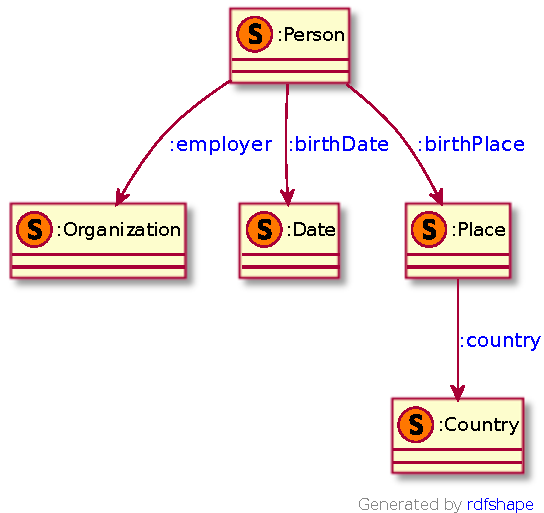
\includegraphics[width=0.4\textwidth]{diagrams/6-5_ShEx.pdf}
    \caption{ShEx schema visualization as UML-like diagrams}
    \label{fig:RDFshape}
\end{figure}

The FAIR (\fb{Findable}, \fb{Accessible}, \fb{Interoperable} and \fb{Reusable}) Guiding principles for data management state that as data's amount, complexity, and rate of creation rise, humans will increasingly need computational assistance to manage it\footnote{\url{https://www.go-fair.org/fair-principles/}}. This is where Wikidata Schemas, or WShEx, could help us address that issue. Wikidata's dumps can be examined in this manner to see if they adhere to a particular schema, obtaining a subset of valid entities as a result. Thus, the community can exchange and reuse data from Wikidata by using schemas, which also serve to improve the quality and usefulness of the data.

ShEx was chosen by Wikibase in 2019 to be the language for describing entity schemas\footnote{\url{https://www.wikidata.org/wiki/Wikidata:Database_reports/EntitySchema_directory}}. As ShEx cannot be used for JSON validation, instead of the Wikibase data model itself, Shape Expressions describe the RDF serialization of Wikibase entities. This implies that the ShEx-based approach is far from the Wikibase data model itself. This issue will be fixed through the solution described in section \ref{section:WShEx}. Observe how the opaque URIs we discussed in section \ref{section:opaqueURIs} are used as the identifiers for specifying Wikidata items.

\begin{code}[ShExC syntax example declaring that nodes of the shape Person must fulfill a schema]
    \inputminted{shex}{code/listings/6-5_wikibase.shex}
\end{code}

\subsubsection{WShEx}
\label{section:WShEx}

As a solution to the problem described before, an extension of ShEx for describing the Wikibase data model was designed. WShEx is a language inspired by ShEx that provides support for the Wikibase data model and can be used to describe and validate Wikibase entities~\cite{https://doi.org/10.48550/arxiv.2208.02697}. What's more, the main motivation for developing this language was to create subsets of Wikidata using a human-readable language.

\begin{code}[ShExC syntax example declaring that nodes of the shape Person must fulfill a schema]
    \inputminted{shex}{code/listings/6-6_wshex.shex}
\end{code}

Figure \ref{fig:WShEx} represents the relationship between ShEx, WShEx and the Wikibase data model. This way, by validating the Wikibase data model through WShEx, we are not only validating the dumps but the system itself.

\begin{figure}[ht]
    \centering
    \includestandalone[width=0.6\textwidth]{diagrams/6-6_WShEx}
    \caption[Relationships between ShEx, WShEx and the Wikibase data model]{Relationships between ShEx, WShEx and the Wikibase data model~\cite{https://doi.org/10.48550/arxiv.2110.11709}}
    \label{fig:WShEx}
\end{figure}

\section{Knowledge Graph Subsets}

Wikidata keeps getting bigger and better. A vast volume of data, like that found in Wikidata, has several benefits but also some drawbacks, including performance. One approach that also provides a snapshot of the contents of Wikidata at a specific point in time is to replicate Wikidata on one's infrastructure~\cite{10.37044/osf.io/wu9et}. However, replicating Wikidata in its entirety is not necessary; instead, subsets might be used to focus on, say, a specific domain. As a substitute for reducing the volume and range of data given by Wikidata, those subsets have become more popular. While maintaining compatibility with the entire Wikidata as the model is retained, handling fewer data enables more complex searches and operations over it.

\begin{definition}[Wikibase subset~\cite{https://doi.org/10.48550/arxiv.2110.11709}]
    Given a Wikibase graph $\Graph=\langle\ItemSet,\PropSet,\DataValueSet,\StmtSet\rangle$, a Wikibase sub-graph is defined as  $\Graph'=\langle\ItemSet',\PropSet',\DataValueSet',\StmtSet'\rangle$ such that: $\ItemSet'\subseteq\ItemSet$, $\PropSet'\subseteq\PropSet$, $\DataValueSet'\subseteq\DataValueSet$ and $\StmtSet'\subseteq\StmtSet$.
\end{definition}

\begin{example}[Example of wikibase subgraph]
    Given the Wikibase graph $\Graph=\langle\ItemSet,\PropSet,\DataValueSet,\StmtSet\rangle$ from example \ref{example:wikibaseGraph}, $\Graph'=\langle\ItemSet',\PropSet',\DataValueSet',\StmtSet'\rangle$ is a Wikibase subgraph of $\Graph$.
\end{example}

\begin{table}[ht]
    \centering
    \documentclass{standalone}
\usepackage{longtable}
% creating some commands for reuse later on :D
\newcommand{\myfont}[1]{\ensuremath{\mathcal{#1}}}

\newcommand{\VertSet}{\myfont{V}}
\newcommand{\NodeSet}{\myfont{N}}
\newcommand{\EdgeSet}{\myfont{E}}
\newcommand{\LabelSet}{\myfont{L}}
\newcommand{\PLabelSet}{\myfont{T}}
\newcommand{\MsgSet}{\myfont{M}}
\newcommand{\None}{\myfont{None}}

\newcommand{\triple}[3]{\ensuremath{\langle #1,#2,#3 \rangle}}
\newcommand{\quadruple}[4]{\ensuremath{\langle #1,#2,#3,#4\rangle}}
\newcommand{\ItemSet}{\myfont{Q}}
\newcommand{\PropSet}{\myfont{P}}
\newcommand{\EntitySet}{\myfont{E}}
\newcommand{\ValueSet}{\myfont{V}}
\newcommand{\DataValueSet}{\myfont{D}}
\newcommand{\StmtSet}{\rho}
\newcommand{\FinSet}[1]{\ensuremath{FinSet(#1)}}
\newcommand{\Graph}{\myfont{G}}

\newcommand{\hrefc}[3][blue]{\href{#2}{\color{#1}{#3}}}%
\newcommand{\elemento}[2]{\ensuremath{\hrefc[violet]{http://www.wikidata.org/entity/#2}{#1}}}
\newcommand{\propiedad}[2]{\ensuremath{\hrefc[blue]{http://www.wikidata.org/entity/#2}{#1}}}
\newcommand{\alanTuring}{\elemento{alanTuring}{Q7251}}
\newcommand{\wilmslow}{\elemento{wilmslow}{Q2011497}}
\newcommand{\town}{\elemento{town}{Q3957}}
\newcommand{\government}{\elemento{government}{Q220798}}
\newcommand{\warringtonLodge}{\elemento{warringtonLodge}{Q20895942}}
\newcommand{\bombe}{\elemento{bombe}{Q480476}}
\newcommand{\unitedKingdom}{\elemento{unitedKingdom}{Q145}}
\newcommand{\computer}{\elemento{computer}{Q11742076}}
\newcommand{\dateOfBirth}{\propiedad{dateOfBirth}{P569}}
\newcommand{\placeOfBirth}{\propiedad{placeOfBirth}{P19}}
\newcommand{\country}{\propiedad{country}{P27}}
\newcommand{\employer}{\propiedad{employer}{P108}}
\newcommand{\discoverer}{\propiedad{discoverer}{P61}}
\newcommand{\dateOfDeath}{\propiedad{dateOfDeath}{P570}}
\newcommand{\placeOfDeath}{\propiedad{placeOfDeath}{P20}}
\newcommand{\timeStart}{\propiedad{timeStart}{P580}}
\newcommand{\timeEnd}{\propiedad{timeEnd}{P582}}
\newcommand{\manufacturer}{\propiedad{manufacturer}{P176}}
\newcommand{\Human}{\elemento{Human}{Q5}}
\newcommand{\instanceOf}{\propiedad{instanceOf}{P31}}

\newcommand{\fb}[1]{\dofb#1}
\newcommand{\dofb}[1]{\textbf{#1}\nobreak\hspace{0pt}}

\newcommand{\mi}[1]{\ensuremath{\mathit{#1}}}

\newcommand{\emptyGraph}{\ensuremath{\emptyset}}
\newcommand{\EmptyGraph}{\ensuremath{\emptyset}}
\newcommand{\addTriple}{\ensuremath{\rtimes}}
\newcommand{\unionGraphs}{\ensuremath{\cup}}
\newcommand\neighs[2]{\ensuremath{neighs(#1,#2)}}
\newcommand\nodes[1]{\ensuremath{nodes(#1)}}
\newcommand{\node}{\mi{n}}
\newcommand{\lbl}{\mi{l}}
\newcommand{\g}{\mi{g}}
\newcommand{\vertex}{\mi{v}}
\newcommand{\msg}{\mi{msg}}
\newcommand{\msgs}{\mi{msgs}}
\newcommand{\labels}{\mi{labels}}
\newcommand{\TripleConstraint}{\mi{TripleConstraint}}
\newcommand{\ShapeReference}{\mi{ShapeReference}}
\newcommand{\ShapeAnd}{\mi{ShapeAnd}}
\newcommand{\ShapeOr}{\mi{ShapeOr}}
\newcommand{\Cardinality}{\mi{Cardinality}}

% Algorithmic definitions
\SetKwProg{Def}{def}{$\,$:}{}
\SetKwProg{Defn}{def}{~$=$}{}
\SetKw{defn}{def}
\newcommand{\DefInline}[2]{\defn #1 = #2}
\SetKwProg{DefnCustom}{\defn}{}{}
\SetKw{Let}{let}
\SetKwInput{KwIn}{Input}
\SetKwFor{ForEach}{foreach}{}{}
\SetKw{Or}{or}
\SetKw{And}{and}
\SetKwIF{If}{ElseIf}{Else}{if}{then}{else if}{else}{endif}
\SetKw{Match}{match}
\SetKw{MyIf}{if}
\SetKw{MyThen}{then}
\SetKw{MyElse}{else}
\SetKw{Case}{case}
\SetKwBlock{Let}{let}{in}
\SetKw{In}{in}
\SetKw{MapTo}{\ensuremath{\;\;\Rightarrow\;\;}}
\SetKwBlock{Block}{}{}
\newcommand{\assign}{\ensuremath{~\mathtt{:=}~}}
\newcommand{\algocomment}[1]{\text{//$\,$#1}}

\newcommand{\blockskip}{\smallskip}
\newcommand{\done}{\ensuremath{\mathit{done}}}

% [algorithm spacing:]
\def\algorithmsize{small}
\def\algorithmheadersize{\algorithmsize}
\renewcommand\AlCapFnt{\normalfont\bfseries\small}
\setlength{\textfloatsep}{1.0ex}
\setlength{\floatsep}{1.0ex}

% Statuses
\newcommand{\Ok}{\ensuremath{Ok}}
\newcommand{\Failed}{\ensuremath{Failed}}
\newcommand{\WaitingFor}[3]{\ensuremath{WaitingFor}(#1,#2,#3)}
\newcommand{\Pending}{\ensuremath{Pending}}
\newcommand{\PendingLs}{\ensuremath{Pending}(ls)}
\newcommand{\Undefined}{\ensuremath{Undefined}}

\newcommand{\Validate}{\ensuremath{Validate}}
\newcommand{\Checked}[2]{\ensuremath{Checked(#1,#2)}}
\newcommand{\WaitFor}[1]{\ensuremath{WaitFor(#1)}}
\newcommand{\status}[2]{\ensuremath{#1(#2)}}
\newcommand{\msgSent}[3]{\ensuremath{#1,#2\rightsquigarrow{}#3}}
\newcommand{\checkLocal}[2]{\ensuremath{checkLocal(#1,#2)}}
\newcommand{\checkLocalOpen}[2]{\ensuremath{checkLocalOpen(#1,#2)}}

\newcommand{\neighbors}[3]{\ensuremath{neighbors}(#1,#2,#3)}
\newcommand{\fracEmpty}[2]{\genfrac{}{}{0pt}{0}{#1}{#2}}
\newcommand{\vProg}{vProg}
\newcommand{\tripleConstraints}[1]{tripleConstraints(#1)}
\newcommand{\rbe}[1]{\ensuremath{rbe(#1)}}
\newcommand{\combine}[2]{\ensuremath{combine(#1,#2)}}
\begin{document}
\begin{tabular}{ccl}
    \ItemSet'      & = \{ & \alanTuring, \wilmslow, \government\hspace{1mm} \}                          \\
    \PropSet'      & = \{ & \placeOfBirth, \employer, \timeStart\hspace{1mm} \}                         \\
    \DataValueSet' & = \{ & {\small 1938}, {\small 1945}\hspace{1mm} \}                                 \\
    $\StmtSet$'    & = \{ & (\alanTuring, \placeOfBirth, \wilmslow, \{\}),                              \\
                   &      & (\alanTuring, \employer, \government, \{\timeStart: 1938 \}),               \\
                   &      & (\alanTuring, \employer, \government, \{\timeStart: 1945 \})\hspace{1mm} \} \\
\end{tabular}
\end{document}
\end{table}

\subsection{ShEx-based Matching generated subsets}

ShEx-based matching comprises using a WShEx schema \myfont{S} as input and includes any nodes whose neighborhood matches any of the shapes from \myfont{S} in the produced subset~\cite{https://doi.org/10.48550/arxiv.2110.11709}. For us to better understand the concept of neighborhood, a formal definition is provided.

\begin{definition}[Neighborhood of a node in a Wikibase graph]
    \label{definition:neighborhood}
    The neighbors of an item $q\in\ItemSet$ in a Wikibase graph $\Graph=\langle\ItemSet,\PropSet,\DataValueSet,\StmtSet\rangle$ are defined as $neighbors(q)=\{(q,p,n,d): \exists{}v\in\StmtSet \wedge v=(q,p,n,d)\}$
\end{definition}

\begin{example}[Neighborhood of \href{https://www.wikidata.org/wiki/Q7251}{Alan Turing (Q7251)}]
    Given the Wikibase graph $\Graph=\langle\ItemSet,\PropSet,\DataValueSet,\StmtSet\rangle$ from example \ref{example:wikibaseGraph}, the neighborhood of \href{https://www.wikidata.org/wiki/Q7251}{Alan Turing (Q7251)} $\in \ItemSet$ is defined as follows:
\end{example}

\begin{table}[ht]
    \centering
    \documentclass{standalone}
\usepackage{longtable}
% creating some commands for reuse later on :D
\newcommand{\myfont}[1]{\ensuremath{\mathcal{#1}}}

\newcommand{\VertSet}{\myfont{V}}
\newcommand{\NodeSet}{\myfont{N}}
\newcommand{\EdgeSet}{\myfont{E}}
\newcommand{\LabelSet}{\myfont{L}}
\newcommand{\PLabelSet}{\myfont{T}}
\newcommand{\MsgSet}{\myfont{M}}
\newcommand{\None}{\myfont{None}}

\newcommand{\triple}[3]{\ensuremath{\langle #1,#2,#3 \rangle}}
\newcommand{\quadruple}[4]{\ensuremath{\langle #1,#2,#3,#4\rangle}}
\newcommand{\ItemSet}{\myfont{Q}}
\newcommand{\PropSet}{\myfont{P}}
\newcommand{\EntitySet}{\myfont{E}}
\newcommand{\ValueSet}{\myfont{V}}
\newcommand{\DataValueSet}{\myfont{D}}
\newcommand{\StmtSet}{\rho}
\newcommand{\FinSet}[1]{\ensuremath{FinSet(#1)}}
\newcommand{\Graph}{\myfont{G}}

\newcommand{\hrefc}[3][blue]{\href{#2}{\color{#1}{#3}}}%
\newcommand{\elemento}[2]{\ensuremath{\hrefc[violet]{http://www.wikidata.org/entity/#2}{#1}}}
\newcommand{\propiedad}[2]{\ensuremath{\hrefc[blue]{http://www.wikidata.org/entity/#2}{#1}}}
\newcommand{\alanTuring}{\elemento{alanTuring}{Q7251}}
\newcommand{\wilmslow}{\elemento{wilmslow}{Q2011497}}
\newcommand{\town}{\elemento{town}{Q3957}}
\newcommand{\government}{\elemento{government}{Q220798}}
\newcommand{\warringtonLodge}{\elemento{warringtonLodge}{Q20895942}}
\newcommand{\bombe}{\elemento{bombe}{Q480476}}
\newcommand{\unitedKingdom}{\elemento{unitedKingdom}{Q145}}
\newcommand{\computer}{\elemento{computer}{Q11742076}}
\newcommand{\dateOfBirth}{\propiedad{dateOfBirth}{P569}}
\newcommand{\placeOfBirth}{\propiedad{placeOfBirth}{P19}}
\newcommand{\country}{\propiedad{country}{P27}}
\newcommand{\employer}{\propiedad{employer}{P108}}
\newcommand{\discoverer}{\propiedad{discoverer}{P61}}
\newcommand{\dateOfDeath}{\propiedad{dateOfDeath}{P570}}
\newcommand{\placeOfDeath}{\propiedad{placeOfDeath}{P20}}
\newcommand{\timeStart}{\propiedad{timeStart}{P580}}
\newcommand{\timeEnd}{\propiedad{timeEnd}{P582}}
\newcommand{\manufacturer}{\propiedad{manufacturer}{P176}}
\newcommand{\Human}{\elemento{Human}{Q5}}
\newcommand{\instanceOf}{\propiedad{instanceOf}{P31}}

\newcommand{\fb}[1]{\dofb#1}
\newcommand{\dofb}[1]{\textbf{#1}\nobreak\hspace{0pt}}

\newcommand{\mi}[1]{\ensuremath{\mathit{#1}}}

\newcommand{\emptyGraph}{\ensuremath{\emptyset}}
\newcommand{\EmptyGraph}{\ensuremath{\emptyset}}
\newcommand{\addTriple}{\ensuremath{\rtimes}}
\newcommand{\unionGraphs}{\ensuremath{\cup}}
\newcommand\neighs[2]{\ensuremath{neighs(#1,#2)}}
\newcommand\nodes[1]{\ensuremath{nodes(#1)}}
\newcommand{\node}{\mi{n}}
\newcommand{\lbl}{\mi{l}}
\newcommand{\g}{\mi{g}}
\newcommand{\vertex}{\mi{v}}
\newcommand{\msg}{\mi{msg}}
\newcommand{\msgs}{\mi{msgs}}
\newcommand{\labels}{\mi{labels}}
\newcommand{\TripleConstraint}{\mi{TripleConstraint}}
\newcommand{\ShapeReference}{\mi{ShapeReference}}
\newcommand{\ShapeAnd}{\mi{ShapeAnd}}
\newcommand{\ShapeOr}{\mi{ShapeOr}}
\newcommand{\Cardinality}{\mi{Cardinality}}

% Algorithmic definitions
\SetKwProg{Def}{def}{$\,$:}{}
\SetKwProg{Defn}{def}{~$=$}{}
\SetKw{defn}{def}
\newcommand{\DefInline}[2]{\defn #1 = #2}
\SetKwProg{DefnCustom}{\defn}{}{}
\SetKw{Let}{let}
\SetKwInput{KwIn}{Input}
\SetKwFor{ForEach}{foreach}{}{}
\SetKw{Or}{or}
\SetKw{And}{and}
\SetKwIF{If}{ElseIf}{Else}{if}{then}{else if}{else}{endif}
\SetKw{Match}{match}
\SetKw{MyIf}{if}
\SetKw{MyThen}{then}
\SetKw{MyElse}{else}
\SetKw{Case}{case}
\SetKwBlock{Let}{let}{in}
\SetKw{In}{in}
\SetKw{MapTo}{\ensuremath{\;\;\Rightarrow\;\;}}
\SetKwBlock{Block}{}{}
\newcommand{\assign}{\ensuremath{~\mathtt{:=}~}}
\newcommand{\algocomment}[1]{\text{//$\,$#1}}

\newcommand{\blockskip}{\smallskip}
\newcommand{\done}{\ensuremath{\mathit{done}}}

% [algorithm spacing:]
\def\algorithmsize{small}
\def\algorithmheadersize{\algorithmsize}
\renewcommand\AlCapFnt{\normalfont\bfseries\small}
\setlength{\textfloatsep}{1.0ex}
\setlength{\floatsep}{1.0ex}

% Statuses
\newcommand{\Ok}{\ensuremath{Ok}}
\newcommand{\Failed}{\ensuremath{Failed}}
\newcommand{\WaitingFor}[3]{\ensuremath{WaitingFor}(#1,#2,#3)}
\newcommand{\Pending}{\ensuremath{Pending}}
\newcommand{\PendingLs}{\ensuremath{Pending}(ls)}
\newcommand{\Undefined}{\ensuremath{Undefined}}

\newcommand{\Validate}{\ensuremath{Validate}}
\newcommand{\Checked}[2]{\ensuremath{Checked(#1,#2)}}
\newcommand{\WaitFor}[1]{\ensuremath{WaitFor(#1)}}
\newcommand{\status}[2]{\ensuremath{#1(#2)}}
\newcommand{\msgSent}[3]{\ensuremath{#1,#2\rightsquigarrow{}#3}}
\newcommand{\checkLocal}[2]{\ensuremath{checkLocal(#1,#2)}}
\newcommand{\checkLocalOpen}[2]{\ensuremath{checkLocalOpen(#1,#2)}}

\newcommand{\neighbors}[3]{\ensuremath{neighbors}(#1,#2,#3)}
\newcommand{\fracEmpty}[2]{\genfrac{}{}{0pt}{0}{#1}{#2}}
\newcommand{\vProg}{vProg}
\newcommand{\tripleConstraints}[1]{tripleConstraints(#1)}
\newcommand{\rbe}[1]{\ensuremath{rbe(#1)}}
\newcommand{\combine}[2]{\ensuremath{combine(#1,#2)}}
\begin{document}
\begin{tabular}{ccl}
    $neighbors(\alanTuring)$ & = \{ & (\alanTuring, \instanceOf, \Human, \{\}),                                                          \\
                             &      & (\alanTuring, \dateOfBirth, {\small 23 June 1912}, \{\}),                                          \\
                             &      & (\alanTuring, \placeOfBirth, \warringtonLodge, \{\}),                                              \\
                             &      & (\alanTuring, \dateOfDeath, {\small 7 June 1954}, \{\}),                                           \\
                             &      & (\alanTuring, \placeOfDeath, \wilmslow, \{\}),                                                     \\
                             &      & (\alanTuring, \employer, \government, \{ \timeStart: {\small 1938}, \timeEnd: {\small 1945} \}) \}
\end{tabular}
\end{document}
\end{table}

To put things simply, a neighborhood of a node in a Knowledge Graph is the set of all the vertices in the graph that are connected to that node. In other words, it is the set of all the nodes that are \textit{directly} connected to the node in question.

\section{Data-flow paradigms}

The main focus of this document is implementing a Big data solution using the Pregel model. However, for a better understanding of it, introducing the MapReduce system will be helpful. Notice that both are meant to be executed in a distributed system. To sum up, the goal of this project is to create a fault-tolerant system making easy to operate on graphs on a massive scale.

\subsection{MapReduce}
\label{section:mapReduce}

Inspired by the map and reduce functions, a MapReduce~\cite{wiki:MapReduce} program is composed of a \textit{map procedure}, where we apply a simple operation to all the elements of a sequence, followed by a \textit{reduce} method, which transforms those elements into a single result. For us to process a graph, we would need to chain MapReduce invocations. Where, for each iteration, map and reduce functions are applied. The main drawback of this approach is the functional nature of the MapReduce model. This means, expressing a graph algorithm as chained MapReduce calls, results in sending the entire state of the graph from one stage to another~\cite{10.1145/1807167.1807184}.

\subsection{Bulk Synchronous Parallel}

During the 1980s, Leslie Valiant worked on ideas for a distributed programming model for parallel computing. In this framework, the execution is divided into a series of \textit{supersteps}. For each superstep, a set of processes running the same piece of code are executed concurrently. As a process completes its execution, a message is generated and sent to other processes. The superstep concludes when all of the procedures are completed. Next, a \textit{barrier synchronization} ensures that all messages have been transferred. At the beginning of the next superstep, all messages are delivered and the aforementioned procedure is repeated. This process will continue until all nodes vote to halt; this is, no more messages are sent to neighboring nodes. It is worth mentioning that processes are not permitted to exchange messages between them when executing a superstep, just at the end. This requirement assures that no deadlocks occur at runtime. Apache Hama\footnote{\url{https://hama.apache.org/}} is a framework for Big data analytics using the Bulk Synchronous Parallel model.

\begin{figure}[ht]
    \centering
    \includestandalone{diagrams/6-7_bsp}
    \caption[Trace of the execution of Pregel for computing the maximum value]{Trace of the execution of Pregel for computing the maximum value~\cite{10.1145/1807167.1807184}}
    \label{fig:pregel}
\end{figure}

\subsection{Pregel model}
\label{section:pregel}

Pregel (\textit{Parallel, Graph and Google}) is a data flow paradigm and system created by Google to handle large-scale graphs. Even though the original system remains proprietary at Google, the computational model was adopted by many graph-processing systems: including Apache Spark. For a better understanding of Pregel, the idea is to \textit{think like a vertex}; this way, for computing the state of a given node, we only depend on the states of its neighboring ones. We will call neighboring vertices of a certain one to those nodes connected to it by an outgoing edge (see definition \ref{definition:neighborhood}). \textit{Thinking like a vertex} could be understood as the \textit{leitmotif} for dividing the problem into several sub-problems: instead of dealing with a huge graph, we just have to solve the problem for smaller graphs: a vertex and its neighboring ones. Notice how a graph to be processed with Pregel may potentially have millions of vertices with billions of edges. More on the size of the Wikibase graphs will be discussed later on.

In comparison to the MapReduce framework, where for each iteration the state of the whole graph must be passed, at each \textit{superstep} -- the way we refer to iterations in Pregel -- each vertex can: send a message to its neighbors, process the received messages (from the previous superstep), and update its state. Summing up, instead of sending the whole state of the graph, we just send messages back and forth. The best way for understanding this is through an example. Let me show you the resulting trace after applying Pregel for computing the maximum value in a graph (see figure \ref{fig:pregel}).

\begin{figure}[ht]
    \centering
    \includestandalone{diagrams/6-8_pregelTrace}
    \caption[Trace of the execution of Pregel for computing the maximum value]{Trace of the execution of Pregel for computing the maximum value~\cite{10.1145/1807167.1807184}}
    \label{fig:pregel}
\end{figure}

Notice that at the beginning of the execution, the state of all the nodes will be set to active. This initial stage is called \textit{superstep 0}. When a vertex is active, it sends a message to its neighbors, which will receive it in the next \textit{superstep}. In this case, the message we are propagating is the largest value that we have learned so far. As an example of that, the second to the left node starts with a value of 6 -- which is the maximum value of the graph -- and sends that number to its neighbors: 3 and 1. In the next \textit{superstep}, the vertices that have received a message have to compare both: the value they store and the received one. This comparison is what it's called the \textit{vProg} function, which will vary from one problem to another. Then, both nodes will update their state to 6. As they have updated their state, they will have to send the new value to its neighbors: beginning another iteration (\textit{superstep}). Notice that at the \textit{superstep 1}, the second to the left node is halted as it doesn't send any other message to its neighbors as its value has not changed. When every node is halted -- inactive -- the execution of the algorithm finishes. In Figure \ref{fig:state} a simplified state machine is shown.

\begin{figure}[ht]
    \centering
    \includestandalone{diagrams/6-9_stateDiagram}
    \caption[Simplified state diagram of a vertex]{Simplified state diagram of a vertex~\cite{10.1145/1807167.1807184}}
    \label{fig:state}
\end{figure}

\subsubsection{Architecture of a Pregel system}

It's quite simple to describe the architecture of a Pregel system. As we have seen, one of the main goals of this model is achieving a parallel execution. This way, a \textit{master} node will divide the graph into several partitions and assign one (or more) of them to each \textit{worker} node. For the \textit{master} to create the partitions it selects a bunch of vertices and all those vertices' outgoing edges; remember: \textit{think like a vertex}.

\begin{figure}[p]
    \centering
    \includestandalone[width=\textwidth]{diagrams/6-10_pregelArchitecture}
    \caption[Architecture of a Pregel system]{Architecture of a Pregel system~\cite{10.1145/3349265}}
    \label{fig:architecture:pregel}
\end{figure}

\part{Design and Implementation of the Pregel solution}

\chapter{Analysis of the existing Pregel solution}
\label{chapter:existing}
\epigraph{\textit{The most important single aspect of software development is to be clear about what you are trying to build.}}{-- \textup{Bjarne Stroustrup}}

In this chapter, we will describe the first implementation of the Pregel solution, exposing the decisions that led to it, as well as the technical debt that we have identified. This first version is part of Labra's publication~\cite{https://doi.org/10.48550/arxiv.2110.11709}.

\section{Technology stack}

For us to describe the technologies used, we have to summarize the needs of the solution first. A large-scale data processing framework is required. What's more, a graph-processing library implementing a Pregel abstraction is also advisable; this way, we can focus on the algorithm for creating the subsets. Finally, it would be ideal if the stated technologies were open-source and well-maintained. Let us describe the chosen stack.

\begin{figure}[ht]
    \begin{subfigure}{.3\textwidth}
        \centering
        
\includegraphics[width=.7\linewidth]{img/7-1_scala.png}
        \caption{Scala programming language}
    \end{subfigure}%
    \hspace*{0.5em}
    \begin{subfigure}{.3\textwidth}
        \centering
        
\includegraphics[width=.7\linewidth]{img/7-2_spark.png}
        \caption{Apache Spark}
    \end{subfigure}%
    \hspace*{0.5em}
    \begin{subfigure}{.3\textwidth}
        \centering
        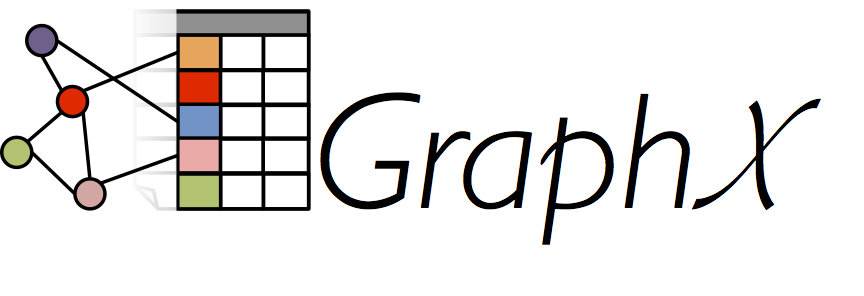
\includegraphics[width=.7\linewidth]{img/7-3_graphx.png}
        \caption{GraphX framework}
    \end{subfigure}%
    \caption{Stack of the different technologies we are using for the first solution}
\end{figure}

\subsection{Scala}

\footnotetext{\url{https://www.scala-lang.org/}}
\footnotetext{\url{https://en.wikipedia.org/wiki/Criticism_of_Java}}

Scala\footnotemark is a high-level programming language combining object-oriented and functional paradigms. Intended to be concise and to answer the majority of Java's complaints.\footnotemark. Allowing operator overloading, better functional support, lazy evaluation and requiring less boilerplate code in general. One of the features that I enjoy the most is pattern matching, which is not supported in Java. What's interesting is that Scala source code can be compiled into Java bytecode, the instruction set of the Java Virtual Machine. This way, a vast ecosystem of Java libraries is available when writing Scala programs. One of the main disadvantages of Scala is that major updates are not backward compatible; this way, programs written in Scala 2.12 are not supported in 2.13. Not to mention that nowadays there exist two major branches of Scala development, namely Scala 2 and 3. Putting this all together, we can conclude that Scala is a bit unstable. This ends up being a hell of a maintenance making loads of open-source projects and libraries get abandoned; we will discuss this later on.

\begin{code}[Hello World written in Scala]
    \inputminted{scala}{code/listings/7-1_helloWorld.scala}
\end{code}

\subsection{Apache Spark}

Apache Spark is a Big data engine with support for several programming languages, including Scala and Python. Aiming to be simple, fast and scalable, it is the most widely-used engine in the industry. The idea behind Spark is to create a Framework that makes parallel jobs over high volumes of data easy to write. It also bundles an engine supporting query optimization which will be discussed later on. For us to understand how Spark works, let's describe its architecture first. It follows the master-slave architecture, the same idea behind the Pregel model, built on top of two abstractions, namely \texttt{Resilient Distributed Dataset (RDD)} and \texttt{Directed Acyclic Graph (DAG)}.

\subsubsection{RDDs (Resilient Distributed Datasets)}

We want to process graphs in parallel; hence, a distributed approach is required to store the graph itself as it is so large to fit in the memory of a single machine. RDDs are necessary for us to address that issue. They are spread in memory or across several machines in a cluster and serve as Apache Spark's primary logical data unit. This method allows a single RDD to be split into numerous logical segments that can then be stored and processed on various cluster machines. RDDs are also lazy-evaluated, which saves time and boosts efficiency. For us to have a better understanding of RDDs, their main features are listed below:

\begin{itemize}
    \itemsep0.25em
    \item \textbf{Resilience or Fault tolerance:} RDDs keep track of data lineage information to automatically restore lost data in the case of failure.
    \item \textbf{Partitioning:} Any existing RDD can be partitioned to generate mutable logical sections. This can be done by performing transformations on the current partitions.
    \item \textbf{Lazy-evaluation:} Even if you define data, it does not load in an RDD. When you call an operation, like count, collect or when you save the output to a file system, transformations are computed.
    \item \textbf{Immutability:} You cannot alter the data that is saved in an RDD since it is in read-only mode. But by applying modifications to the current RDDs, you can produce new RDDs.
    \item \textbf{In-memory computation:} To allow faster access, RDD stores every immediately created data in the main memory.
\end{itemize}

After reviewing the key aspects of RDDs, let us try to improve our understanding by describing the environment that supports this abstraction. As stated in the introduction, Spark is constructed on top of RDDs; this includes abstractions such as DataFrames and Datasets which are developed using them.  Every computation in Spark is carried out by RDDs under the hood. In other words, they are Spark's most basic building blocks. Some advantages of RDDs are their simplicity, capacity to import data from heterogeneous sources, ease of caching, and the ability to apply transformations to the data stored functionally. However, as we are essentially storing Java objects (or Scala ones), they consume rather large amounts of memory, garbage collection is necessary, and serialization is required for data storage and retrieval. This issue is especially critical for larger datasets since the time to serialize/deserialize grows in proportion to the amount of data stored. More into this will be discussed later on.

\subsubsection{DAG (Directed Acyclic Graph)}

The main difference between Spark and Hadoop MapReduce, whose limitations lead to the creation of the former, is the DAG Scheduler. In the context of Apache Spark, a Directed Acyclic Graph, DAG for short, is a set of \textit{Vertices}, representing an RDD partition, and \textit{Edges}, representing the operations to be applied. This graph is later transformed into stages by the DAG Scheduler, where each stage contains a series of tasks to be executed in parallel. As we had seen in section \ref{section:mapReduce}, the main issue with MapReduce is having to store the result of each intermediate node, in a DAG architecture this is not required.

\begin{figure}[ht]
    \centering
    \includestandalone[width=0.65\textwidth]{diagrams/7-1_apacheSparkArchitecture}
    \caption[Architecture of Apache Spark]{Architecture of Apache Spark\footnotemark}
    \label{fig:architecture:apacheSpark}
\end{figure}

\footnotetext{\url{https://spark.apache.org/docs/0.9.1/cluster-overview.html}}

\subsection{GraphX}

A graph processing framework integrated with Apache Spark was suggested as GraphX in 2014. Its API contains a Pregel fork that is used to implement several algorithms, including PageRank. GraphX exposes an API for graphs based on RDDs~\cite{https://doi.org/10.48550/arxiv.2110.11709}.

\subsubsection{The GraphX implementation of Pregel}

GraphX provides several built-in operators for graphs\footnote{\url{https://spark.apache.org/docs/latest/graphx-programming-guide.html\#graph-operators}}. We will use the following in the rest of the paper:

\begin{itemize}
    \setlength\itemsep{1em}
    \item \mintinline[fontsize=\small]{scala}{mapVertices(g: Graph[·\VertSet·,·\EdgeSet·], f: (Id,·\VertSet·)·$\rightarrow$··\VertSet·)): Graph[·\VertSet·,·\EdgeSet·]}
          \begin{itemize}
              \item[$\blacksquare$] \textbf{Description:} Transforms each vertex attribute in the graph using the map function. It maps every pair \texttt{(id,v)} -- which are the vertices of \texttt{g} -- into \texttt{(id,f(v))}.
              \item[!] \textbf{Note:} The new graph has the same structure. As a consequence, the underlying index structures can be reused.
          \end{itemize}
    \item \mintinline[fontsize=\small]{scala}{mapReduceTriplets(g: Graph[·\VertSet·,·\EdgeSet·], m: (·\VertSet·,·\EdgeSet·,·\VertSet·)·$\rightarrow$·(Id,·\MsgSet·)), r: (·\MsgSet·,·\MsgSet·)·$\rightarrow$··\MsgSet·)): RDD[Id,·\MsgSet·]}
          \begin{itemize}
              \item[$\blacksquare$] \textbf{Description:} Takes a user-defined map function \texttt{m} which is applied to each triplet and can yield messages which are aggregated using the reduce function \texttt{r}.
          \end{itemize}
    \item \mintinline[fontsize=\small]{scala}{joinVertices(g: Graph[·\VertSet·,·\EdgeSet·], msgs: RDD[Id,·\MsgSet·], f: (Id,·\VertSet·,·\MsgSet·)·$\rightarrow$··\VertSet·)): Graph[·\VertSet·,·\EdgeSet·]}
          \begin{itemize}
              \item[$\blacksquare$] \textbf{Description:} Joins the vertices with the input RDD and returns a new graph with the vertex properties obtained by applying the user-defined map function to the result of the joined vertices. Vertices without a matching value in the RDD retain their original value.
          \end{itemize}
\end{itemize}

The GraphX Pregel implementation is defined iteratively where each iteration is usually called a superstep, taking as input a \texttt{Graph}[\VertSet, \EdgeSet] and the following parameters:

\begin{itemize}
    \itemsep0.5em
    \item \texttt{initialMsg}: the message each vertex will receive at the initial iteration.
    \item \texttt{vProg}: the user-defined vertex program function which is run on each vertex and computes a new value for it. During the first iteration, the \texttt{vProg} is invoked on all vertices. On subsequent iterations it is invoked only on those active vertices; that is, those receiving messages.
    \item \texttt{sendMsg}: the user-defined function applied to all the out edges of vertices receiving a message in the current iteration. To put it simply, a function computing the messages to be sent to the neighbors of a node for the next iteration.
    \item \texttt{mergeMsg}: the user-defined function that is applied to two incoming messages and merges them into one.
\end{itemize}

Below is the pseudo-code of the Pregel operator as implemented in GraphX:

\begin{pseudocode}[The Pregel model as implemented in GraphX]
    \includestandalone{code/algorithms/7-1_pregel}
\end{pseudocode}

It is worth noting that the Pregel operator in GraphX is a \textit{bulk-synchronous} parallel messaging abstraction at a high level. The Pregel operator performs a sequence of supersteps in which vertices receive their inbound message set, calculate a new value for the vertex, and then send messages to their neighbors. Take a look at the first two lines of the pseudo-code above to see how the initial messages for each vertex are received and calculated for iteration 0. Messages, unlike Pregel, are calculated concurrently: note the second and fifth lines of the above snippet. Vertices that receive no messages are skipped. The Pregel operator ends the iteration and returns the final graph when there are no messages left, as seen in the third line of the snippet above. The previously described constraints allow GraphX to perform some additional optimization.

\section{PSchema: Pregel + ShEx generated subsets}

The next paragraphs will describe the ShEx validation algorithm based on Pregel. This approach is based on the assumption that a ShEx schema $\langle  \mathcal{L},\sigma \rangle$ is provided,  with each label $l \in \mathcal{L}$ identifying a \texttt{Shape Expression}.

\begin{figure}[H]
    \centering
    \includestandalone[width=0.6\textwidth]{diagrams/7-2_pregelState}
    \caption[State diagram representing the different states in \texttt{vProg}]{State diagram representing the different states in \texttt{vProg}~\cite{https://doi.org/10.48550/arxiv.2110.11709}}
    \label{fig:state:pregel}
\end{figure}

According to figure \ref{fig:state:pregel}, nodes might be active if they have received some messages, or inactive if they have not received any messages. Certain sub-states are necessary for us to produce a more accurate answer based on Knowledge Graph validation. The algorithm in the Pregel approach is in charge of annotating each node $n\in\mathcal{V}$ with a status map expressing the validation progress for specific labels. A more detailed description of the possible values that the \texttt{Status} can take is provided:

\begin{center}
    \begin{tabular}{ccll}
    $Status$ & ::=    & \texttt{Undefined}                  & Default status                                                         \\
             & $\mid$ & \texttt{Ok}                         & Node conforms to the schema                                            \\
             & $\mid$ & \texttt{Failed}                     & Node does not conform to the schema                                    \\
             & $\mid$ & \texttt{Pending}                    & Requested to be validated                                              \\
             & $\mid$ & \texttt{WaitingFor($ds$,$ok$,$fs$)} & Waiting for some neighbors                                             \\
             &        &                                     & $ds$ = list dependents neighbors                                       \\
             &        &                                     & $ok$ = list of conformant neighbors                                    \\
             &        &                                     & $fs$ = list of non conformant neighbors                                \\
             &        &                                     & where $ds$, $oks$, $failed$ $\in\VertSet\times\PropSet\times\LabelSet$
\end{tabular}
\end{center}

Putting this all together, the algorithm starts by mapping every node to the status which associates any label $l \in \mathcal{L}$ to \texttt{Undefined}, this is the \textit{initial message.} Then, it runs the iterative Pregel algorithm using the following functions:

\begin{enumerate}
    \itemsep0.5em
    \item \texttt{sendMsg}: this function is in charge of sending messages to the neighbors of a node. It is responsible for asking the neighbors to validate the node against a specific label. The message is a tuple containing the label $l$ and the status of the node $n$ for that label $l$.
    \item \texttt{mergeMsg}: this function is in charge of merging the messages received by a node. It is responsible for merging the status of the node $n$ for a specific label $l$ with the status of the node $n$ for that label $l$ received from a neighbor.
    \item \texttt{vProg}: see table \ref{vProg} for a more detailed reference.
\end{enumerate}

Once the algorithm has finished, it replaces the status of any node that is \texttt{Pending} with \texttt{WaitingFor} by looking at the status of its neighbors. This is the last step to ensure that the algorithm has finished. The algorithm returns the graph with the status of each node for each label.

\begin{pseudocode}[Pregel-based ShEx validation pseudocode]
    \includestandalone{code/algorithms/7-2_pregelShEx}
\end{pseudocode}

\begin{table}
    \centering
    
\begin{tabular}{c}
    \inference[$$]
    {\fracEmpty{
            \msgSent{(n,m)}{\lbl}{\Validate}
        }{
            \status{m}{\lbl}=s\in\{\Undefined, \Pending\}
    }                                             & \checkLocal{\lbl}{n}=r\in\{\Ok,\Failed\}
    }
    {\status{m'}{\lbl}=r}

    \\ \\

    \inference[$$]
    {\fracEmpty{\msgSent{(n,m)}{\lbl}{\Validate}}
        {\status{m}{\lbl}=r\in\{\Undefined,\Pending\}
    }                                             & \checkLocal{\lbl}{n}=\PendingLs
    }
    {\fracEmpty{\status{m'}{l}=\Undefined}{\status{m'}{l'}=\Pending\,\,\forall{l'}\in{}ls}}

    \\ \\

    \inference[$$]
    {\fracEmpty{
            \msgSent{(n,m)}{\lbl}{\Validate}}
        {
            \status{m}{\lbl}=r\in\{\Ok,\Failed\}
        }
    }
    {\status{m'}{\lbl}=r}

    \\ \\
    % This is to stop the recursive case....if we request to validate a node for which we are already waiting for, we assume it is valid
    \inference[$$]
    {\fracEmpty{
            \msgSent{(n,m)}{\lbl}{\Validate}
        }{
            \status{m}{\lbl}=\WaitingFor{ds}{oks}{fs}
        }
    }
    {\status{m'}{\lbl}=\Ok}

    \\ \\

    \inference[$$]
    {\fracEmpty{
            \msgSent{(n,m)}{\lbl}{\Checked{oks}{fs}}}
        {
            \status{m}{\lbl}=\WaitingFor{ds}{oks'}{fs'}
    }                                             & ds\setminus(oks\cup{}fs)\neq{}\emptyset
    }
    {\status{m'}{\lbl}=\WaitingFor{ds}{oks\cup{}oks'}{fs\cup{}fs'}}

    \\ \\

    \inference[$$]
    {\fracEmpty{\msgSent{(n,m)}{\lbl}{\Checked{oks}{fs}}}
    {\status{m}{\lbl}=\WaitingFor{ds}{oks'}{fs'}} &
        ds\setminus(oks\cup{}fs)=\emptyset
    }
    {\status{m'}{\lbl}=\neighbors{\lbl}{oks\cup{}oks'}{fs\cup{}fs'}}
\end{tabular}\\


    \caption{Definition of \texttt{vProg} for Pregel-based ShEx validation}
\end{table}
\label{vProg}

\section{Architectural decision record}

In this section, we will discuss the architectural decision record for this project. We will cover the main decisions that have been made throughout the development process and the reasons behind them. The goal is to provide a clear understanding of the project's architecture and the reasoning behind it.

\subsection{DataFrames vs RDDs}

\subsubsection{Status}

\texttt{Superseded}

\subsubsection{Context}

The first decision we have to make was whether to use DataFrames or RDDs. As we have seen in the previous section, both solutions have their pros and cons. The main advantage of RDDs is that they are a more mature API, and therefore, they are more stable and better documented. However, DataFrames are a higher-level abstraction that allows us to write more concise code. In the end, we decided to use DataFrames because they are the future of Spark. RDDs are a lower-level API that is not going to be developed further. In the next paragraph, we will discuss the reasons behind this decision in more detail.

The pros and cons of RDDs and DataFrames are summarized in the following enumeration:

\begin{enumerate}
    \itemsep0.5em
    \item \textbf{For RDDs}: the RDD-based API is based on the functional programming paradigm, and the algorithm is written using higher-order functions. This is, the code of the RDD-based solution is readable even if you have no prior knowledge of Apache Spark. Moreover, as the information is kept in the form of Java objects, the data flow is exposed in the same way that it is in any other Java application.
    \item \textbf{Against RDDs}: the memory usage in RDD-based solutions is far from optimum. The operations to be performed become less efficient as we must serialize and deserialize the data at each iteration of the algorithm. Not to mention the lack of a query execution optimizer, as well as the lack of data homogeneity due to RDDs' being schema-less.
\end{enumerate}

\subsubsection{Rationale}

We have chosen the DataFrame-based solution because:

\begin{itemize}
    \itemsep0.5em
    \item \textbf{DataFrames are the future of Spark}: as we have mentioned before, RDDs are a lower-level API that is not going to be developed further. DataFrames are a higher-level abstraction that allows us to write more concise code.
    \item \textbf{DataFrames are more efficient}: DataFrames are more efficient than RDDs because they are based on a logical plan, and therefore, they can be optimized by the query execution optimizer. Moreover, DataFrames are stored in a columnar format, which allows us to perform operations on a single column without having to load the entire dataset into memory.
\end{itemize}

\subsubsection{Consequences}

By choosing the DataFrame-based solution we will need to invest more time in learning and understanding the API. Additionally, we will need to fine-tune our application's data model to use the DataFrame-based API efficiently.

However, we believe that by choosing the DataFrame-based solution we will be able to write more concise code and achieve better performance.

\chapter{Refactoring the Pregel-based algorithm}
\label{chapter:refactoring}
\epigraph{\textit{The business changes. Technology changes. The team changes. The team members change. Change is not the problem, per se, because change is going to happen; the problem, rather, is the inability to cope with change when it comes.}}{-- \textup{Kent Beck}}

During the early stages of the development, the first steps we followed were highly related to polishing and improving the solution described in the previous chapter. This was a challenging problem that resulted in a change in the project's direction, which will be detailed later.

\section{Technology stack}

As I've mentioned earlier, the purpose of this second solution was to improve what was already implemented. This way, we kept most of the stack untouched. The sole change was the replacement of GraphX with its DataFrame equivalent library named GraphFrames.

\begin{figure}[ht]
    \centering
    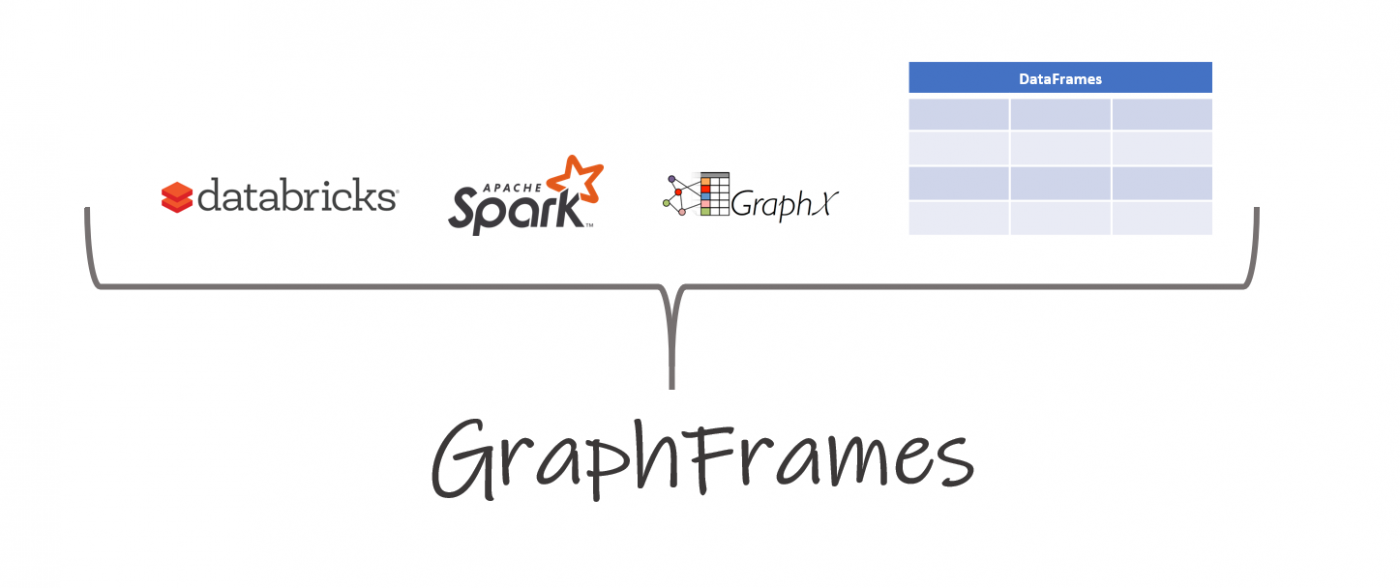
\includegraphics[width=.7\linewidth]{img/8-1_graphframes.png}
    \caption[Stack of the different technologies we are using for the second solution]{Stack of the different technologies we are using for the second solution\footnotemark}
\end{figure}

\footnotetext{\url{https://adatis.co.uk/graphframes/}}

\subsection{Row-based vs. column-based storage}

What we have seen thus far is one of the most common approaches for storing data: row-oriented databases. However, there is another approach that has been gaining traction during the past few years, namely, columnar storage. In the former, data is organized by records, keeping all the information related to a particular entity close to each other in memory. In the latter, data is organized by columns, keeping all the values for a particular attribute close to each other in memory. This is especially relevant when we are working with large amounts of data, as we can perform operations over a particular column without having to load the whole row -- for each entity -- into memory.

Row-oriented databases are the way to go when reading or writing entire rows is the most common operation. This is the case for \texttt{OLTP (Online Transaction Processing)} systems, where we are usually working with small amounts of data. On the other hand, column-oriented databases are the way to go when we are working with \texttt{OLAP (Online Analytical Processing)} systems, where we are usually working with large amounts of data, as we have said before. As an example, let's imagine we have a table with the following schema: \texttt{<ID, name, age, address>}. Having that said, let us assume we have the following data in our table:

\begin{table}[ht]
    \centering
    \begin{tabular}{|c|c|c|c|}
        \hline
        \rowcolor[HTML]{EFEFEF}
        \texttt{ID} & \texttt{name} & \texttt{age} & \texttt{address}            \\ \hline
        1           & John          & 25           & \textit{1234 Main St.}      \\ \hline
        2           & Jane          & 30           & \textit{5678 Main St.}      \\ \hline
        3           & Angel         & 23           & \textit{1234 Secondary St.} \\ \hline
        4           & Eve           & 23           & \textit{5678 Secondary St.} \\ \hline
    \end{tabular}
    \caption{Table with some data}
\end{table}

In a more traditional row-based database the data is stored by rows, such that the first column of a row will be next to the last attribute of the previous one. According to this, we will have the following layout in memory:

\begin{table}[ht]
    \centering
    \begin{tabular}{|c|c|}
        \hline
        \multicolumn{1}{|l|}{\cellcolor[HTML]{EFEFEF}}                                 & 1                           \\ \cline{2-2}
        \multicolumn{1}{|l|}{\cellcolor[HTML]{EFEFEF}}                                 & John                        \\ \cline{2-2}
        \multicolumn{1}{|l|}{\cellcolor[HTML]{EFEFEF}}                                 & 25                          \\ \cline{2-2}
        \multicolumn{1}{|c|}{\multirow{-4}{*}{\cellcolor[HTML]{EFEFEF}\textbf{Row 1}}} & \textit{1234 Main St.}      \\ \hline
        \multicolumn{1}{|l|}{\cellcolor[HTML]{EFEFEF}}                                 & 2                           \\ \cline{2-2}
        \multicolumn{1}{|l|}{\cellcolor[HTML]{EFEFEF}}                                 & Jane                        \\ \cline{2-2}
        \multicolumn{1}{|l|}{\cellcolor[HTML]{EFEFEF}}                                 & 30                          \\ \cline{2-2}
        \multicolumn{1}{|c|}{\multirow{-4}{*}{\cellcolor[HTML]{EFEFEF}\textbf{Row 2}}} & \textit{5678 Main St.}      \\ \hline
        \multicolumn{1}{|l|}{\cellcolor[HTML]{EFEFEF}}                                 & 3                           \\ \cline{2-2}
        \multicolumn{1}{|l|}{\cellcolor[HTML]{EFEFEF}}                                 & Angel                       \\ \cline{2-2}
        \multicolumn{1}{|l|}{\cellcolor[HTML]{EFEFEF}}                                 & 23                          \\ \cline{2-2}
        \multicolumn{1}{|c|}{\multirow{-4}{*}{\cellcolor[HTML]{EFEFEF}\textbf{Row 3}}} & \textit{1234 Secondary St.} \\ \hline
        \multicolumn{1}{|l|}{\cellcolor[HTML]{EFEFEF}}                                 & 4                           \\ \cline{2-2}
        \multicolumn{1}{|l|}{\cellcolor[HTML]{EFEFEF}}                                 & Eve                         \\ \cline{2-2}
        \multicolumn{1}{|l|}{\cellcolor[HTML]{EFEFEF}}                                 & 23                          \\ \cline{2-2}
        \multicolumn{1}{|c|}{\multirow{-4}{*}{\cellcolor[HTML]{EFEFEF}\textbf{Row 4}}} & \textit{5678 Secondary St.} \\ \hline
    \end{tabular}
    \caption{Row-based storage}
\end{table}

This way, writing to a row store is an optimized operation. To put it into perspective, let me show you an example. Let's assume we want to add a new record to our table, namely, \texttt{<5, Bob, 25, 1234 Main St.>}. In this case, we will just have to append the new record at the end of the table, as we can see in figure \ref{table:row-based-storage}. Note that the ellipsis stands for the rest of the table, which is not shown for the sake of simplicity.

\begin{table}[ht]
    \centering
    \begin{tabular}{|c|c|}
        \hline
        \multicolumn{2}{|c|}{$\cdots$}                                                    \\ \hline
        \cellcolor[HTML]{EFEFEF}                                 & 5                      \\ \cline{2-2}
        \cellcolor[HTML]{EFEFEF}                                 & Bob                    \\ \cline{2-2}
        \cellcolor[HTML]{EFEFEF}                                 & 25                     \\ \cline{2-2}
        \multirow{-4}{*}{\cellcolor[HTML]{EFEFEF}\textbf{Row 5}} & \textit{1234 Main St.} \\ \hline
    \end{tabular}
    \caption{Inserting a new record in row-based storage}
\end{table}
\label{table:row-based-storage}

This proves that row-oriented storage is very efficient when we want to add new records to our table. However, if we want to read a specific \textit{column}, we will have to read the entire table, which is not performant. For example, if we want to read the \texttt{name} column, we will load all five rows into memory and then pull out the second attribute of each one of them. As you can see, this approach lacks efficiency as we are loading a lot of data that we are not going to use. To address this issue, column-based storage was designed. In this case, the data is stored by columns, such that all the elements of each row will be next to each other in memory. According to this, and following the same example as before, we will have the following disk layout:

\begin{table}[ht]
    \centering
    \begin{tabular}{|c|c|}
        \hline
        \cellcolor[HTML]{EFEFEF}                                   & 1                           \\ \cline{2-2}
        \cellcolor[HTML]{EFEFEF}                                   & 2                           \\ \cline{2-2}
        \cellcolor[HTML]{EFEFEF}                                   & 3                           \\ \cline{2-2}
        \multirow{-4}{*}{\cellcolor[HTML]{EFEFEF}\texttt{ID}}      & 4                           \\ \hline
        \cellcolor[HTML]{EFEFEF}                                   & John                        \\ \cline{2-2}
        \cellcolor[HTML]{EFEFEF}                                   & Jane                        \\ \cline{2-2}
        \cellcolor[HTML]{EFEFEF}                                   & Angel                       \\ \cline{2-2}
        \multirow{-4}{*}{\cellcolor[HTML]{EFEFEF}\texttt{name}}    & Eve                         \\ \hline
        \cellcolor[HTML]{EFEFEF}                                   & 25                          \\ \cline{2-2}
        \cellcolor[HTML]{EFEFEF}                                   & 30                          \\ \cline{2-2}
        \cellcolor[HTML]{EFEFEF}                                   & 23                          \\ \cline{2-2}
        \multirow{-4}{*}{\cellcolor[HTML]{EFEFEF}\texttt{age}}     & 23                          \\ \hline
        \cellcolor[HTML]{EFEFEF}                                   & \textit{1234 Main St.}      \\ \cline{2-2}
        \cellcolor[HTML]{EFEFEF}                                   & \textit{5678 Main St.}      \\ \cline{2-2}
        \cellcolor[HTML]{EFEFEF}                                   & \textit{1234 Secondary St.} \\ \cline{2-2}
        \multirow{-4}{*}{\cellcolor[HTML]{EFEFEF}\texttt{address}} & \textit{5678 Secondary St.} \\ \hline
    \end{tabular}
    \caption{Column-based storage}
\end{table}

This way, if we want to read a specific column, we will only have to read the one we are interested in. For example, if we want to read the \texttt{name} column, we will just retrieve the second one, which is much more efficient than reading the entire table. However, if we want to append a new record, we will have to add a new entry to the end of each column, leading to a slower insertion. For example, if we want to add the record \texttt{<5, Bob, 25, 1234 Main St.>} to our table, we will add the entries to each column as seen in figure \ref{tab:column_based}. Note that the ellipsis stands for the rest of the entries of each column, which are not shown for the sake of simplicity.

\begin{table}[ht]
    \centering
    \begin{tabular}{|c|c|}
        \hline
        \cellcolor[HTML]{EFEFEF}                                   & $\cdots$               \\ \cline{2-2}
        \multirow{-2}{*}{\cellcolor[HTML]{EFEFEF}\texttt{ID}}      & 5                      \\ \hline
        \cellcolor[HTML]{EFEFEF}                                   & $\cdots$               \\ \cline{2-2}
        \multirow{-2}{*}{\cellcolor[HTML]{EFEFEF}\texttt{name}}    & Bob                    \\ \hline
        \cellcolor[HTML]{EFEFEF}                                   & $\cdots$               \\ \cline{2-2}
        \multirow{-2}{*}{\cellcolor[HTML]{EFEFEF}\texttt{age}}     & 25                     \\ \hline
        \cellcolor[HTML]{EFEFEF}                                   & $\cdots$               \\ \cline{2-2}
        \multirow{-2}{*}{\cellcolor[HTML]{EFEFEF}\texttt{address}} & \textit{1234 Main St.} \\ \hline
    \end{tabular}
    \caption{Inserting a new record in column-based storage}
    \label{tab:column_based}
\end{table}

Putting this all together, row-based databases will be more efficient when performing operations such as \texttt{SELECT * FROM table WHERE id = 1}, as we only need to read the first row. On the other hand, columnar stores will be more efficient when performing operations such as \texttt{SELECT SUM(age) FROM table}, as we only need to read the third column. A typical use-case for row-based databases is systems where the most common operations are any of: \texttt{Create-Read-Update-Delete}. Following into this, row-based databases are commonly used in traditional DBMS such as \texttt{MySQL} or \texttt{PostgreSQL}; to name an example, row-oriented storage excels at \textit{e-commerce} applications where we are required to load whole rows into memory, that is, we may need to retrieve the name, description and price of every item in the shop, or in the case of having to perform frequent insertions to the database. On the other hand, a typical use-case for column-based databases is systems where the most common operations are aggregations and complex queries in general. Following into this, column-based databases are commonly used in data warehouses such as \texttt{Amazon Redshift} or \texttt{Google BigQuery}; to name an example, column-oriented storage excels at \textit{business intelligence} applications where we are required to perform aggregations over a particular column, more precisely, we may need to retrieve the total revenue of the shop, Which is the case for our solution. As we are performing aggregations over columns for each iteration of the Pregel model. This is why we decided to move from row-based to column-oriented storage.

\subsection{GraphFrames}

To continue with what we have been discussing so far, we will now introduce GraphFrames. As its name goes, \texttt{GraphFrames} is a package for Apache Spark providing support for DataFrame-based Graphs and operations over them. According to the introductory lines, the main goal of this stage of the development was to move our solution one step further in the abstraction level, from a solution based on RDDs to another based on DataFrames. From the ground up, we always believed RDDs weren't the go-to. What's more, RDDs are discouraged as they seem to be outdated in comparison to DataFrames and Datasets. More into this will be discussed in the next section. According to the description of the GraphFrames library, this API is similar to GraphX, except, instead of being built on top of RDDs, they are based on DataFrames. However, the fact that the Pregel implementation bundled in the GraphFrames API  has not been updated since 2018, makes us feel cautious about this approach.

\subsection{DataFrames and Datasets}

From Spark version 1.3 onwards, what was once known as SchemaRDDs are now referred to as DataFrames. That may give us an idea of what a DataFrame is. In that sense, they are RDDs provided some Schema for the data that is collected. With the help of this schema, DataFrames may be seen as rows with uniform structure: columns. Whereas RDDs are more akin to objects, DataFrames are closer to a table in a database. This is quite relevant, as managing schemas to describe the information allows us to perform operations over data in a more efficient manner when compared to using Java serialization. It is worth mentioning that from Spark version 2.0 onwards, DataFrames can be understood as a type alias for \texttt{Dataset[Row]}, as they merged both APIs. In that sense, Datasets can be seen as the combination of the best of both worlds: with the appearance of a Java object from the outside, but with the shape of a table in RDBMS internally.

We now have a clear vision of what a DataFrame is. The problem is that even though they provide some nice features for data wrangling: schemas allow us to establish contracts so consumers know exactly the shape of the data they are working with, they are not so nicely implemented currently. Not only Apache Spark has no official support for working with DataFrame-based Graphs: notice GraphFrames is required, but the variety of supported types is scarce: including primitive types and Dates. Long has been discussed in this sense, but nothing has changed since 2015\footnote{\url{https://issues.apache.org/jira/browse/SPARK-7768}}. To clarify this, let's put it into perspective.

\label{sec:encoders}
\subsubsection{Encoders and User-defined Types}

Working with simple data structures is a trivial task in Apache Spark. What is not so easy to handle are custom data types. If the DataFrame cannot implicitly retrieve an \texttt{Encoder}, the user will be required to provide one. This is needed for Spark SQL to infer the schemas of the data we are working with. The more complex the data structure, the harder it is for the programmer to write an appropriate serialization/deserialization mechanism. Notice how this solution is far from efficient as it is based on serialization for data storage and retrieval, something we were trying to avoid when we dropped the RDD-based solution. Another possibility could be writing your own \texttt{User-defined types}, which can be understood as \textit{wrappers} for the actual type. However, the amount of boilerplate code needed, and the complexity of the data to be stored prevents us from writing an appropriate solution.

As we have mentioned earlier, two main possible solutions arise for the problem of handling complex data: \textit{Custom encoders} and \textit{User-defined types}. It is a requirement for this solution not only to handle complex data but unsupported, as we are not only trying to store complex data structures but types that are not currently supported by the DataFrame API. This is a crucial argument against this DataFrame-based solution as we need to store URLs, which aren't currently backed by Spark SQL. The problem is that both of the provided solutions are inefficient. First, collection Encoders tend to act as bottlenecks in terms of performance. To follow up on this, storing non-standard objects in Spark is a mess\footnote{\url{https://stackoverflow.com/questions/36648128/how-to-store-custom-objects-in-dataset}}. The latest version of the framework supports primitive types and dates, as have already mentioned. The currently accepted solution in this sense consists of serializing objects using the \texttt{kryo} encoder which stores them as flat binary objects, preventing us from accessing concrete columns without deserializing the binary. This last matter is especially crucial as messaging in Pregel is built on top of aggregates over particular columns. Hence, we would need to serialize and deserialize every stored item for each iteration. Thus, a  complex and inefficient encoder is not the solution we need. See figure \ref{fig:wikibaseClassDiagram} for an expanded description of Wikibase's data model as implemented in WShEx.

\begin{code}[User-defined types as implemented in Apache Spark]
    \inputminted{scala}{code/listings/8-1_udt.scala}
\end{code}

As noted in the first line of the example above, the description of User-defined types is annotated as an unstable API meant for developers. This implies that in minor Spark versions, the API may change or be eliminated. The use of it is at the user's own risk. As a consequence, if we follow this approach, we will end up with an unstable solution. Not only that but the processes for serializing and deserializing, along with the SQL schema -- which is no longer inferred by Scala's reflection system -- should be explicitly defined. Having said that, by defining our User-defined types, we're only establishing the wrapper, and yet no relationship is established between the real object and the User-defined type in the eyes of Spark's engine. To deal with this, we have two options: annotating the class we want to encapsulate or explicitly registering it. The former requires that the programmer has access to the class being wrapped. An ineffective technique that has been superseded by the latter since Spark 2.0. What's striking here is that it took Spark developers 6 years to come up with an answer in this regard. The API for user-defined types is essentially unmaintained, and dealing with custom objects in Spark is the framework's weak point. More on this was covered in the previously mentioned issue\footnote{\url{https://issues.apache.org/jira/browse/SPARK-7768}}.

\begin{code}[Registration of an User-defined type in Apache Spark]
    \inputminted{scala}{code/listings/8-2_udtRegistration.scala}
\end{code}

The issue here is the complexity of the data structures we use. According to the design in figure \ref{fig:wikibaseClassDiagram}, storing both \texttt{Statements} and \texttt{Entities} presents two major challenges. To begin, as the items stored require a fixed structure and we would like to polymorphically treat \texttt{Properties} and \texttt{Items} -- both -- as \texttt{Entities}, we need a mapping to convert from an object-oriented model to the relational paradigm. In this regard, we suggest \textit{Single Table Inheritance}\footnote{\url{https://en.wikipedia.org/wiki/Single_Table_Inheritance}}; that is, using a single table containing all the fields of all the child classes. The issue here is that we would end up with a solution in which rows contain redundant data: as many \texttt{NULL} values as different fields in child classes that are not the actual type for a certain row. Although it is a straightforward approach, it is inefficient. Second, this technique leads to a circular dependency\footnote{\url{https://en.wikipedia.org/wiki/Circular_dependency}} in which \texttt{Entities} include many \texttt{LocalStatements} that hold \texttt{Qualifiers} that may enclose \texttt{Entities}. When you define a schema for this problem, you eventually wind yourself in an infinite recursion where \texttt{Entities} have \texttt{Entities}. In conclusion, User-defined types offer a poor solution that causes several challenging issues.

\begin{figure}[ht]
    \centering
    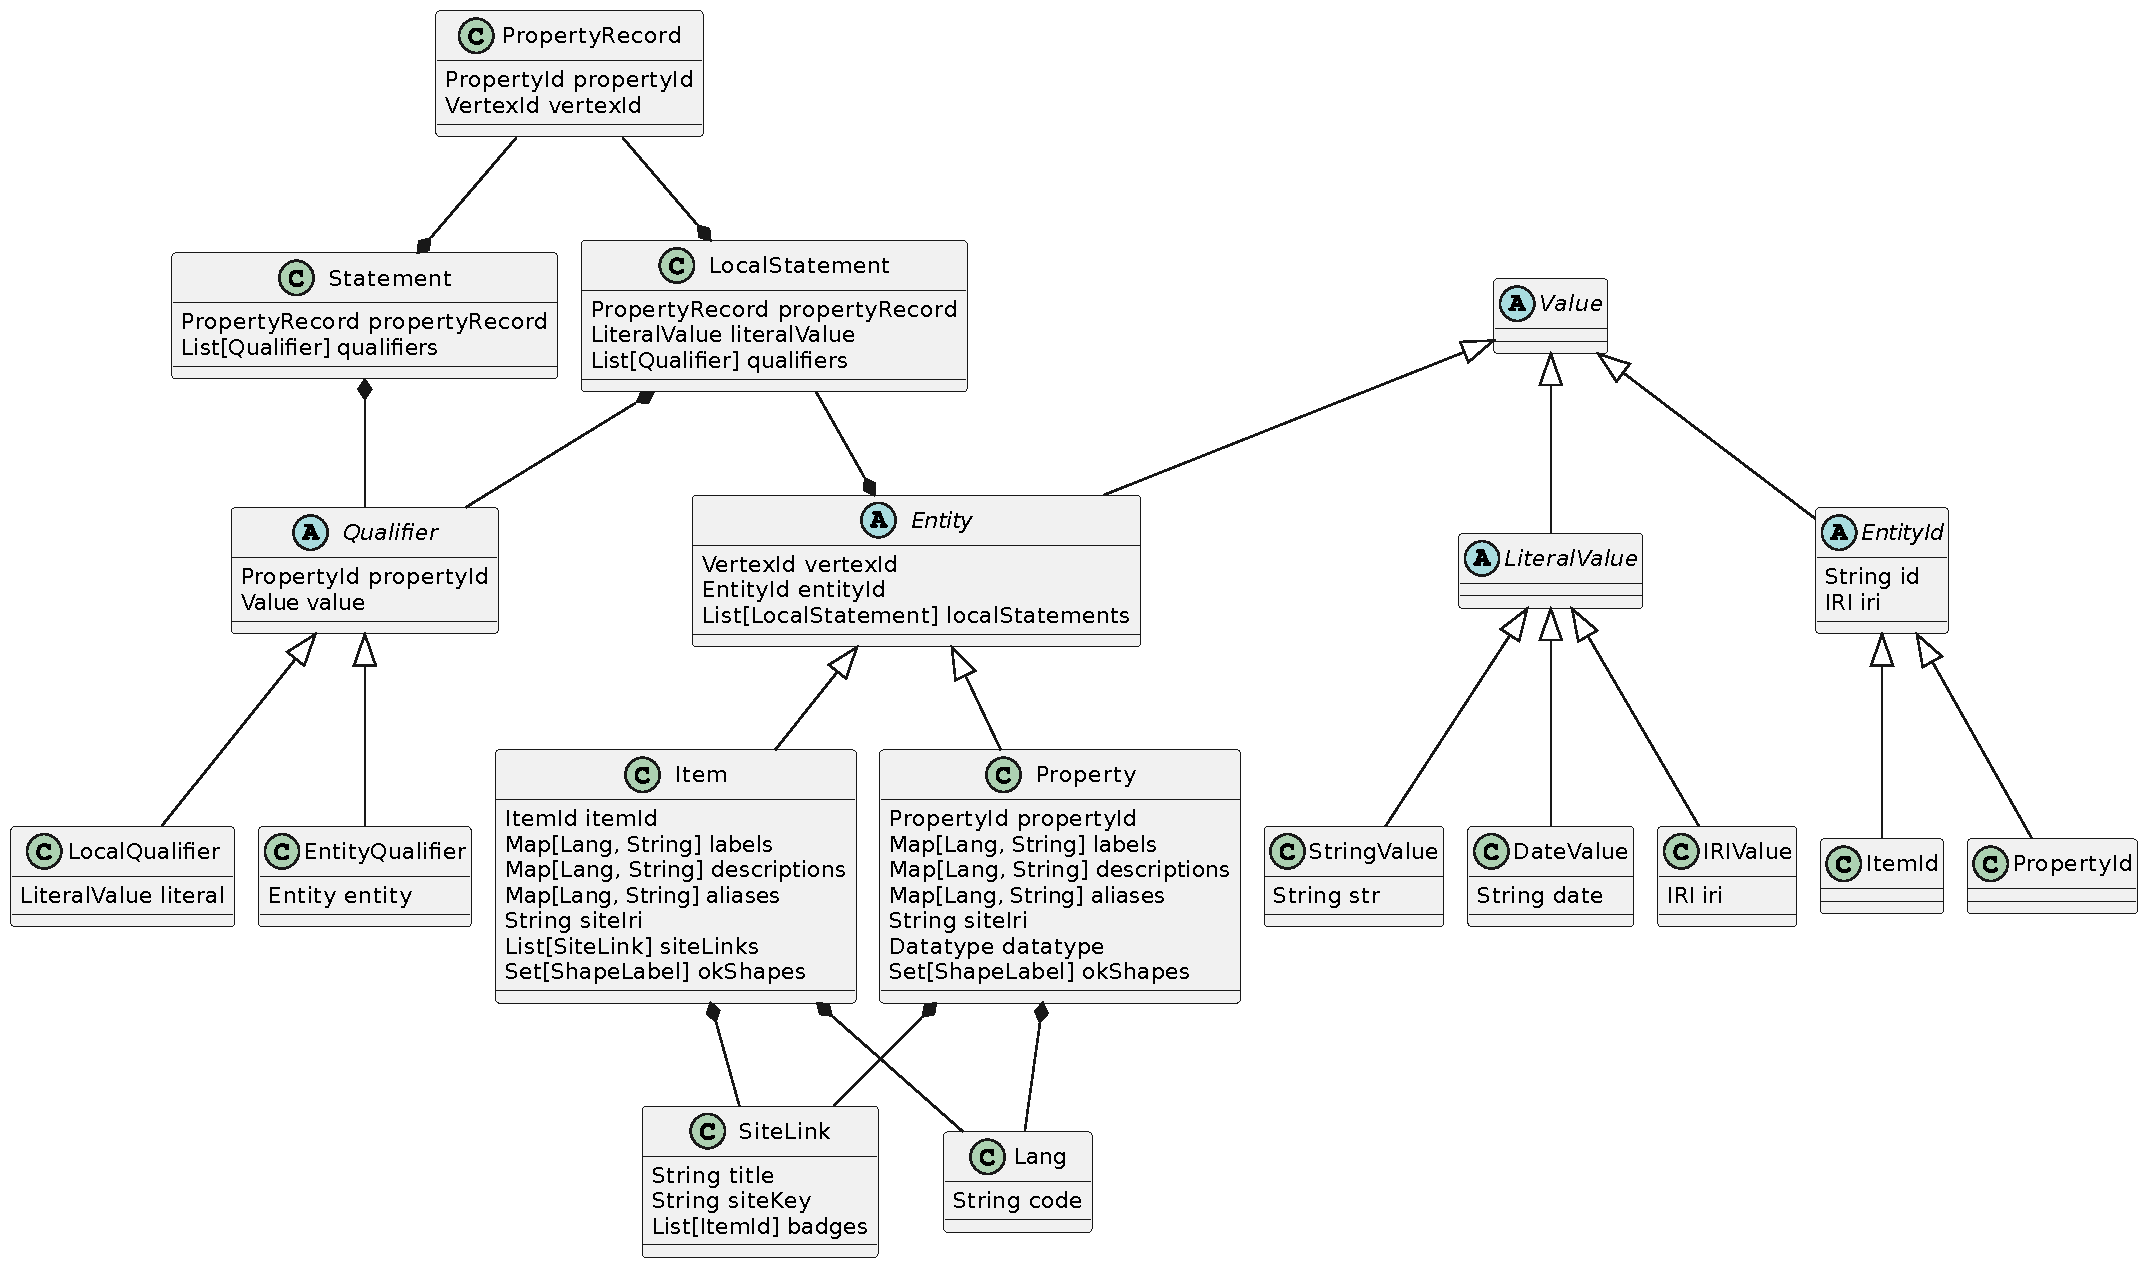
\includegraphics[width=\textwidth]{diagrams/8-1_wikibaseClassDiagram.pdf}
    \caption[Class diagram of the Wikibase data model as implemented in WShEx]{Class diagram of the Wikibase data model as implemented in WShEx\footnotemark}
    \label{fig:wikibaseClassDiagram}
\end{figure}
\footnotetext{\url{https://github.com/weso/shex-s}}

At this point, we can agree that we have ended up in a pitfall. This is, we have identified a challenge in storing intricate data structures in Spark. Additionally, we have examined the two primary approaches to tackle this issue and explained why they are unsuitable for our specific situation. An alternative approach is required, specifically, simplifying the data model we are currently dealing with. In the following chapter, we will delve into the solution we have found to address this problem.

\section{Architectural decision record}

In this section, we will discuss the architectural decision record for this project. We will cover the main decisions that have been made throughout the development process and the reasons behind them. The goal is to provide a clear understanding of the project's architecture and the reasoning behind it.

\subsection{Scala as the programming language}

\subsubsection{Status}

\texttt{Accepted}

\subsubsection{Context}

The first decision we made was to use Scala as the programming language for the development of the solution. This decision was made based on the following reasons:

\begin{enumerate}
    \itemsep0.5em
    \item \textbf{Functional programming paradigm}: Scala is a functional programming language. This means that it is based on the concept of functions as first-class citizens. This allows us to write more concise and readable code. It also allows us to write it in a more declarative manner, which is easier to reason about. This is especially important when working with distributed systems, as it allows us to write code that is easier to parallelize, especially when using a master-worker architecture.
    \item \textbf{JVM-based}: Scala is a JVM-based language. This means that it runs on the Java Virtual Machine. This allows us to use all the Java libraries and tools available. This is especially important when working with distributed systems, as we can use the Spark framework.
    \item \textbf{Existing knowledge and solution}: We have previous experience with Scala, and we have already implemented a solution for this problem in it. This allows us to reuse the code we have already written and the knowledge we have already acquired.
\end{enumerate}

However, Scala has some drawbacks that we need to take into account, and that we started to notice during the development process:

\begin{enumerate}
    \itemsep0.5em
    \item \textbf{Performance}: Scala is not a performant language. It is not as fast as Rust. This means that it is not a good choice for high-performance applications that are meant to run on single-node machines, note that in the next chapter, we will describe the importance of this.
    \item \textbf{Tooling}: even if Scala is a JVM-based language, provided that it has the same tooling as Java, the maintenance of the libraries is not as good as it is for the latter. This means that it is not a good choice for large-scale applications, where we rely on the maintenance of the libraries.
    \item \textbf{Documentation}: from our experience, the documentation for Scala is not as good as it is for other languages. Meaning that maintaining and learning a new technology is harder than it is for other languages.
\end{enumerate}

On the opposite, we have chosen Rust as the programming language for the implementation of the solution. The reasons behind this decision are enumerated in the following section.

\subsubsection{Rationale}

We have chosen Rust because:

\begin{itemize}
    \itemsep0.5em
    \item \textbf{Performance}: Rust is a performant language. It is as fast as C++. This means that it is a good choice for high-performance applications that are meant to run on single-node machines.
    \item \textbf{Memory-safety}: Rust is a memory-safe language.
    \item \textbf{Parallelization}: provided that we are no longer using Spark, and, our solution is not based on the master-worker architecture, we need to parallelize the solution ourselves. Rust is a good choice for this, as it is a functional programming language.
\end{itemize}

\subsubsection{Consequences}

We will have to rewrite the solution in Rust if we want to use it in a production environment. This is because the performance of the current solution is not good enough for us to release it. We will also have to rewrite the solution in Rust if we want to use it in a large-scale environment.

\subsection{Spark as the distributed computing framework}

\subsubsection{Status}

\texttt{Accepted}

\subsubsection{Context}

The second decision we made was to use Spark as the distributed computing framework for this project. As we have already mentioned, we are trying to build a solution on top of the DataFrames API. The thing is that this API relies on the Scala reflection system, which is not as performant as it should be. We have already described this issue in section \ref{sec:encoders}. Hence, we need to find an alternative distributed computing framework that allows us to work with DataFrames. Note that the problem with the DataFrames API is related to the type system, not to the columnar orientation. This is, what we are trying to achieve is finding an alternative to Spark's DataFrame API.

\subsubsection{Rationale}

We have chosen \texttt{pola-rs} because:

\begin{itemize}
    \itemsep0.5em
    \item \textbf{Written in Rust}: \texttt{pola-rs} is written in Rust, meaning that it is a good choice for high-performance applications that are meant to run on single-node machines.
    \item \textbf{Rust API}: \texttt{pola-rs} has a Rust API, meaning that we can use it in our Rust-based solution.
\end{itemize}

\subsubsection{Consequences}

We will have to rewrite the whole solution, as we are no longer using Spark.

More into this in chapter \ref{chapter:analysis}.

\part{Is Distributed Computing the solution?}

\chapter{Analysis of the Rust solution}
\label{chapter:analysis}
\epigraph{\textit{The most damaging phrase in the English language is "we have always done it this way".}}{-- \textup{Grace Hopper}}

We have examined two distinct Scala and Apache Spark-based solutions up to this point. Both were, as we have mentioned, far from ideal. We have to start from scratch if we want to find a more sophisticated solution.

\section{Technology stack}

\begin{figure}[ht]
    \centering
    \newsavebox\mybox
    \savebox{\mybox}{
\includegraphics[width=.3\linewidth]{img/9-1_rust.jpg}}
    \begin{subfigure}{.3\textwidth}
        \centering
        \usebox{\mybox}
        \caption{Rust programming language}
    \end{subfigure}%
    \hspace*{0.1em}
    \begin{subfigure}{.3\textwidth}
        \centering
        \vbox to \ht\mybox{%
            \vfill
            
\includegraphics[width=.9\linewidth]{img/9-2_duckdb.png}
            \vfill
        }
        \caption{DuckDB}
    \end{subfigure}%
    \hspace*{0.1em}
    \begin{subfigure}{.3\textwidth}
        \centering
        \vbox to \ht\mybox{%
            \vfill
            
\includegraphics[width=.8\linewidth]{img/9-3_polars.pdf}
            \vfill
        }
        \caption{Pola-rs}
    \end{subfigure}%
    \caption{Stack of the different technologies we are using for the third solution}
\end{figure}

\label{section:rust}
\subsection{Rust}

Rust is a multi-purpose and high-level programming language. Its primary focus is on performance, memory safety, and concurrency. In this perspective, Rust might be considered a modern language, and as of March 18th, 2023, the most recent stable release is version 1.68. For achieving memory safety and concurrency, both at the same time, Rust prevents data races through a \textit{borrow checker} that tracks the object and allows each memory position to have only one owner at a time. Rust is popular for systems programming, and was included by the Linux kernel in December 2022, but it also has some high-level functional constructs like pattern-matching and the neatly implemented \texttt{Enums}.

The key features of Rust are:

\begin{enumerate}
    \itemsep0.5em
    \item \textbf{Performance:} It accomplishes this by employing a static memory management strategy rather than a garbage collector, using \textit{ownership} instead. This means that the compiler decides when memory is allocated and released at compile time. Rust can produce incredibly effective code as a result.
    \item \textbf{Memory safety:} Rust is designed to be memory safe. It achieves this by using a \textit{borrow checker}. This means that the compiler determines at compile time when memory is accessed, allowing Rust to prevent memory issues like use-after-free and double-free.
    \item \textbf{Concurrency:} Rust is designed to be \textit{concurrent}. This means that Rust programs can be executed in partial order, or out-of-order, without affecting the outcome. This allows the parallel execution of the concurrent units, significantly increasing the performance of the program in multi-threaded systems.
\end{enumerate}

An example of a simple \textit{Hello World} program written in Rust is shown below.

\begin{code}[Hello World written in Rust]
    \inputminted{rust}{code/listings/9-1_helloWorld.rs}
\end{code}

Having that said, let me make a brief remark on some of the features that I loved the most when working with Rust. Regarding the compiler, first of all, it is very strict and will not allow you to compile your code if it is not safe. This is a great feature because it will prevent you from having to deal with runtime errors. Secondly, the compiler is very helpful and will give you a lot of information about the error that you are facing. This is, it will help you to understand what is going on and how to fix it. Lastly, the compiler is very smart and will optimize your code for you. This is a great feature because it makes you write code that is fast and efficient, without even realizing it.

Regarding the language itself, first of all, Rust is heavily inspired by functional programming languages. Hence, many of the features that you will find in Rust are also present in Scala. Recall that one of the features that I loved the most about the latter was \textit{pattern matching} and Rust has it too. Secondly, Rust has a very powerful type system. What I enjoy about this feature is the way Rust handles errors. This is, by returning either a \texttt{Result} or an \texttt{Option} type, Rust forces you to handle errors and nullable functions safely. When combined with the \texttt{?} operator, error handling becomes very easy and concise. What's more, you can manage both through the \texttt{match} statement, a really clean approach. Lastly, concurrency is implemented following the same design principles as in Go, that is, it adheres to the \textit{share memory by communicating} principle: \textit{Do not communicate by sharing memory; instead, share memory by communicating}. This means that Rust uses \textit{channels} to communicate between threads, which is a very safe and efficient way of doing it. Rust's concurrency system reminds me of the idea behind the Pregel model, where the data is partitioned and sent to the different workers, which are the threads in this case. Then, workers can communicate with each other through the channels, which is the same as sending messages between workers in the Pregel model.

\subsection{DuckDB}

Conversely, DuckDB is an in-process SQL OLAP database management system written in C++ that is intended to be integrated into other applications. This means that DuckDB follows the ACID model and supports popular SQL constructs like window functions, table expressions, and JSON. Additionally, it is column-oriented storage and was created with analytical queries in mind. The impact of this last remark on the scope of our project will be explained further below. Being a project that is only a few years old, DuckDB is still being actively developed.

The key features of DuckDB are:

\begin{enumerate}
    \itemsep0.5em
    \item \textbf{In-process:} DuckDB is an embedded database that runs in the same process as the application. This means that there is no separate server process that needs to be started, stopped, or configured. The application can directly interact with DuckDB via a C API. Notably, this API is designed to be identical to the one utilized by SQLite. As a result, DuckDB can seamlessly substitute SQLite as a plug-and-play alternative.
    \item \textbf{OLAP or On-Line Analytical Processing:} DuckDB is designed for OLAP workloads. It is optimized for analytical queries that scan large amounts of data and perform complex aggregations. This is in contrast to OLTP, or On-Line Transaction Processing, which is optimized for transactional workloads with a high number of small transactions. DuckDB is not a suitable replacement for a traditional OLTP database like PostgreSQL or MySQL.
    \item \textbf{Columnar:} DuckDB is a columnar database. This means that data is stored in columns instead of rows. This can dramatically minimize the amount of data that needs to be read from memory because DuckDB can now only read the columns needed for a query. The vectorized query execution method, which enables incredibly quick query execution, benefits from the column orientation as well. Last but not least, the compression efficiency of the columnar storage format can help to further reduce the quantity of data that needs to be read from memory.
\end{enumerate}

\subsection{Pola-rs}

Pola-rs is a fast and memory-efficient DataFrame library for Rust. It is built on top of Apache Arrow, a cross-language development platform for in-memory data. This means that data can be shared between languages without the need for serialization or deserialization. Many well-known data science and analytics frameworks, such as Apache Parquet, Apache Spark, Dask, and Pola-rs, employ Apache Arrow. Putting it all together, Pola-rs is a DataFrame implementation written in Rust, a data structure that is commonly used in data science and analytics.

The key features of Pola-rs are:

\begin{enumerate}
    \itemsep0.5em
    \item \textbf{Zero-copy:} Pola-rs is a DataFrame library that uses Apache Arrow as the memory model. This means that Pola-rs does not copy data when performing operations on the DataFrame. Instead, it manipulates the metadata of the underlying Arrow array. This makes Pola-rs very fast and memory efficient.
    \item \textbf{Parallel execution:} Pola-rs is designed to be parallel. This means that Pola-rs can execute operations on several threads at the same time. This allows Pola-rs to take advantage of multi-core systems, resulting in faster execution.
    \item \textbf{Lazy evaluation:} Pola-rs is designed to be lazy. This means that Pola-rs does not execute operations until they are needed. This allows Pola-rs to avoid unnecessary computations, resulting in faster execution.
    \item \textbf{Query optimization:} Pola-rs' Lazy API optimizes the query plan for it to be executed faster. This means that Pola-rs can optimize queries by reordering operations and removing unnecessary ones. This allows queries to be executed faster.
    \item \textbf{Streaming:} Pola-rs is designed to allow streams from external files. This means that Pola-rs can process data in batches read from an external file or database. This allows Pola-rs to process data without having to load it all into memory first, resulting in the possibility of processing larger datasets, even if they do not fit in memory.
\end{enumerate}

\section{Extract-Transform-Load}

As discussed in the preceding chapter, we have encountered challenges related to the data model we are currently handling. The primary issue arises from the data's lack of a convenient structure for manipulation. Circular dependencies and recursive structures have proven to be problematic in our case. Consequently, we have decided to migrate the data to a relational database, which would provide a more organized and valid data model. The initial step involves extracting the data from the JSON file and transforming it into a format that facilitates seamless processing. This is where the Extract-Transform-Load (ETL) process becomes crucial.

The Extract-Transform-Load (ETL) process is a data integration method aiming at extracting data from one or more sources, transforming it, and loading the result into a target system. An ETL process is a critical component of data-intensive applications, as having properly structured and valid data has a strong impact on the quality of the results and the performance of the system. With that said, the ETL process is used in data migration projects, where data is moved from one system to another. This last remark is important because it is the case of our project, where we are willing to move data from a JSON file to a relational database.

\begin{figure}[ht]
    \centering
    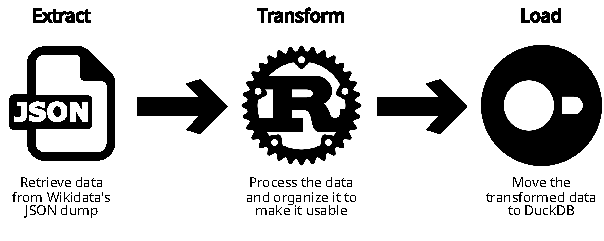
\includegraphics[width=0.8\textwidth]{diagrams/9-1_etl.pdf}
    \caption{Extract-Transform-Load (ETL) process description}
\end{figure}

\subsection{Extract}

The first step of the ETL process is the extraction of data from the source system. This step is responsible for connecting to the source system and retrieving the data. The source system can be a database, a file, or even a web service. In our case, we want to extract the data from a JSON dump, so we will need to connect to the file system and read the data from the file. See section \ref{section:json_dump} for more details.

\subsection{Transform}

The second step of the ETL process is the transformation of data. This step is responsible for converting the data from its source format to the target format. It is also responsible for cleaning the data, removing duplicates, and performing other operations to ensure that the data is valid and consistent. In our case, we want to transform the data from a JSON format to DuckDB. Not only that, but we also have to store the data in a way that is consistent with the knowledge graph model. This means that we have to extract the entities and relationships from the data and represent them in a graph format. See section \ref{section:wd2duckdb_design} for more details.

\subsection{Load}

The third and final step of the ETL process is the loading of data into the target system. It is responsible for connecting to the target system and inserting the data. In our case, we want to load the data into a DuckDB database. See section \ref{section:duckdb_load} for more details.

For us to accomplish what we have just described, we will need to use a tool that can perform the ETL process. In our case, we will implement one ourselves using Rust. This tool will be responsible for extracting data from a JSON file, transforming it into a relational format, and loading it into a DuckDB database. The tool will be called \texttt{wd2duckdb}. See chapter \ref{chapter:wd2duckdb} for more details.

\section{Knowledge Graph Subsets}

Moreover, merely having our data stored in a relational database is insufficient. It is crucial to remember that our objective is to develop an algorithm capable of validating Knowledge graphs. As a result, we must establish a system that allows us to query the graph in a Pregel-like manner. Currently, there is no existing implementation written in Rust and based on DataFrames that aligns with our requirements. Hence, we will introduce a new system called \texttt{pregel-rs} to fulfill this need. Additionally, we will also require an algorithm for generating subsets, which will be named \texttt{pschema-rs}. Further information can be found in Chapter \ref{chapter:pschema}.

\chapter{From Wikidata JSON dumps to DuckDB}
\label{chapter:wd2duckdb}
\epigraph{\textit{Information flow is what the Internet is about. Information sharing is power. If you don't share your ideas, smart people can't do anything about them, and you'll remain anonymous and powerless.}}{-- \textup{Vint Cerf}}

We have seen thus far the two main export formats supported by Wikidata, namely, RDF and JSON. However, none of them are suitable for analytical queries. In this chapter, we will explore the possibility of exporting Wikidata in a columnar format, as we have mentioned in the previous chapter, DuckDB is the perfect candidate for this task. This is, we will create a Rust-based solution for exporting Wikidata to DuckDB.

\section{The issue with JSON and other text-based formats}
\label{section:issue}

JSON is a text-based format, and as such, the data that is stored inside a JSON file is not compressed in any way. This means that the size of the file is directly proportional to the size of the data. This is not a problem for small datasets, but it becomes an issue when we are dealing with larger information repositories. As we have seen in the introductory chapter a Wikidata JSON dump is around \texttt{1.5 TB} in size when uncompressed. See Chapter \ref{chapter:intro} for a more detailed explanation. The challenge lies in the inability to load such a massive file into the memory of a single machine. Even if feasible, the loading process would be time-consuming and incur substantial expenses for renting a suitable machine. As a result, a binary format is required to store the information. This is where DuckDB comes into play. Despite the need to load the database into memory (recall, DuckDB is an in-process or embedded database), the repository's size is considerably smaller than that of the JSON file, often differing by several orders of magnitude. DuckDB achieves this by utilizing a columnar database structure, enabling more efficient compression of the data compared to a text-based format. This compression advantage is the primary reason driving our decision to export Wikidata to DuckDB.

It is worth mentioning that Wikidata JSON dumps follow a structure where each line of the file stores a single object. This provides the advantage of being able to parse the file line by line, which is quite convenient. However, there is a drawback: every line in the dump includes redundant boilerplate information related to the JSON object schema. In other words, we may have hundreds of millions of lines, all containing the same boilerplate code. Instead of having a header with the object schema, it is repeated in every line of the document. This redundancy significantly impacts the memory efficiency of JSON files. While JSON is excellent for sharing information, it is not the most efficient option for storage purposes.

\section{wd2duckdb}

Now that we have a clear understanding of the scope of the project, we can start working on the design of the tool in charge of transforming the Wikidata JSON dumps into a DuckDB file. For us to do so, some decisions are made. First, we are interested in storing only one of the translations of each Wikidata entity; that is, we are going to store only one of the labels, descriptions and aliases of each item. However, the language of choice can be modified\footnote{\url{https://github.com/angelip2303/wd2duckdb/blob/master/wikidata-rs/src/lib.rs\#L20}}. Second, we are going to store only the statements that are not deprecated. Apart from that, the rest of the information is going to be stored as it is.

\label{section:wd2duckdb_design}
\subsection{Design}

The tool is going to be divided into two main parts. The first one is going to be in charge of parsing the Wikidata JSON dump and extracting the information that we are interested in. The second part is going to be in charge of storing the information in a DuckDB database. The idea is to allow backends to be interchangeable; that is, several implementations for other drivers should be implemented without actually changing the existing code. However, for the sake of simplicity, we are going to focus on DuckDB for the time being.

\label{section:json_dump}
\subsubsection{Parsing the JSON dump}

The first part of the tool is going to be in charge of parsing the Wikidata JSON dump and extracting the information that we are interested in. In this manner, we are going to parse the JSON dump line by line. Recall, each line of the dump contains a single JSON object, which is -- indeed -- a Wikidata entity. It is worth noting that the entities in the array are not sorted in any way. This is, we have to be aware that the first entity in the dump is not necessarily the first Wikidata entity, namely, \texttt{Q1}. Thus, our solution should not rely on the order of the entities in the dump. What's more, a certain entity of the dump can refer to another that has not been parsed yet. Hence, we must be able to handle this situation as well.

Having that said, it is worth mentioning that a Wikidata dump can contain hundreds of millions of entities. This means that we cannot store all that information in memory. Hence, we must find a way to append the information to the resulting database as we parse the dump.

\label{section:duckdb_load}
\subsubsection{Storing the information in DuckDB}

The second part of the tool is going to be in charge of storing the information we have retrieved in the resulting database. Hence, we are going to load the following information into DuckDB:

\begin{itemize}
    \itemsep0.5em
    \item \textbf{Wikidata IDs}: As we had seen in section \ref{section:wikibase_graphs}, Wikidata IDs consist of a type prefix \texttt{Q}, \texttt{P} or \texttt{L}, for identifying Entities, Properties or Lexemes, followed by a sequence of numbers. There exist other two types of IDs, namely, \texttt{F} and \texttt{S}, for identifying Forms and Senses, respectively. A more detailed discussion on this topic will be presented later on.
    \item \textbf{Labels}: We are going to store the labels of the entities in the same table where we store the IDs.
    \item \textbf{Descriptions}: We are storing the descriptions of the entities in the same table where we store the IDs.
    \item \textbf{Statements}: We are going to store the statements of the entities in a separate table so that we can build the graph later on. The idea is to store the ID of the source entity, the ID of the property and the ID of the destination entity. In this manner, we will end up with two main tables: one for storing the entities, or vertices, and another one for storing the statements, or edges. Several other tables are going to be created for storing data relative to the information that comes with the statements, such as qualifiers, references, ranks, etc. However, for the time being, we are going to focus on the main tables.
\end{itemize}

According to what we have just described, we are going to end up with a database that contains two main tables: one for storing the entities, or vertices, and another one for storing the statements, or edges. The schema of the database is depicted in figure \ref{fig:schema}.

\begin{figure}[ht]
    \centering
    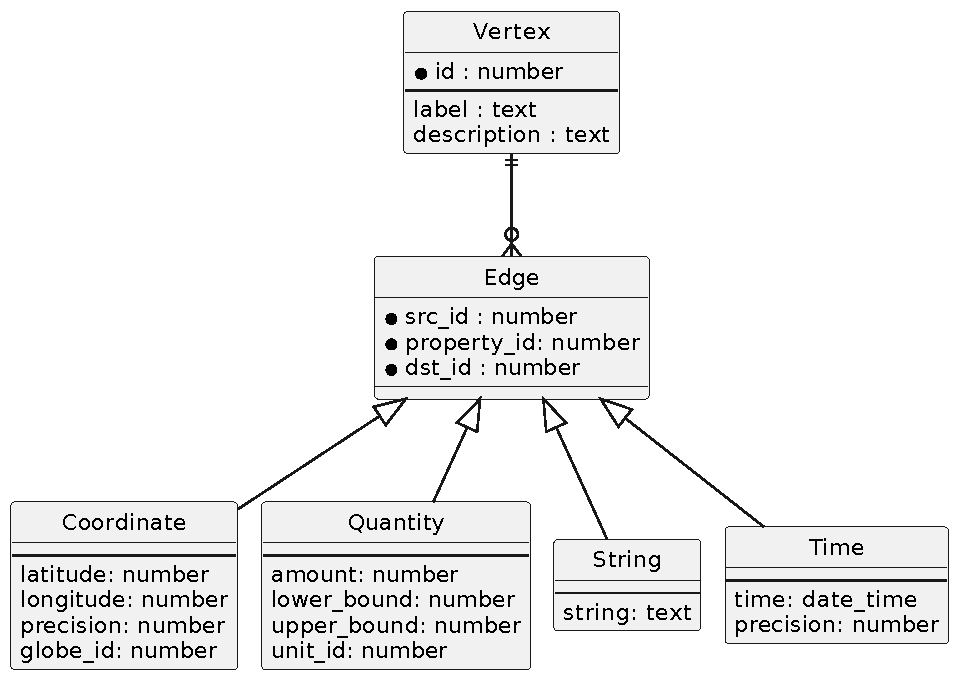
\includegraphics[width=.75\linewidth]{figures/diagrams/10-1_wd2duckdb.pdf}
    \caption{Entity-relationship diagram of the Database created by the \texttt{wd2duckdb} tool}
    \label{fig:schema}
\end{figure}%

\subsection{Implementation of the \texttt{wd2duckdb} tool}

Once we have a better understanding of the design of the tool. Now, we can start working on the implementation of it. The idea is to create a Rust-based solution that can be used as a library or as a command-line tool. This CLI will act as a wrapper for the library and is responsible for calling it, as well as handling command-line inputs such as the source JSON and the target file. Through \texttt{crates.io}\footnote{\url{https://crates.io/crates/wikidata-rs}}, we aim to make the library available to other Rust projects. This is, we are looking to decouple the library from the binary for other backends to be implemented on top of the same traits.

The most relevant aspect of the implementation revolves around the insertion of the processed Wikidata entities into the database. To accomplish this, we will leverage the powerful \texttt{duckdb-rs}\footnote{\url{https://crates.io/crates/duckdb}} library, which provides a Rust interface for DuckDB. Note that, it is based on the same interface as the SQLite driver for Rust. The plan is to utilize this library to create the necessary database and tables, and then employ it again to insert the data into it. The diagram in Figure \ref{fig:activity} illustrates the implementation of the \texttt{wd2duckdb} tool.

To insert the data into the database, we first need to establish a connection to it by creating a \texttt{Connection} object. Subsequently, we create the \texttt{Statement} and execute the corresponding SQL statement, specifically an insert one. However, the main concern arises executing the aforementioned statements for each entity, as it would severely impact the tool's performance due to the need for creating numerous connections to the database, corresponding to the number of lines in the JSON dump. To address this issue, we employ a transactional approach. By creating a transaction and executing the insert statements within it, we can greatly enhance the tool's performance. Once all the entities have been inserted, we commit the transaction. Notably, this approach requires only a single connection to the database. It becomes even more convenient when utilizing the \texttt{duckdb-rs} library, as it provides an \texttt{Appender} struct. The \texttt{Appender} not only encapsulates the transaction but also optimizes the data insertion process by buffering the data and inserting it into the database in batches. Consequently, the tool's performance is further improved. This is the recommended approach for inserting large amounts of data into a database.

\begin{figure}[p]
    \centering
    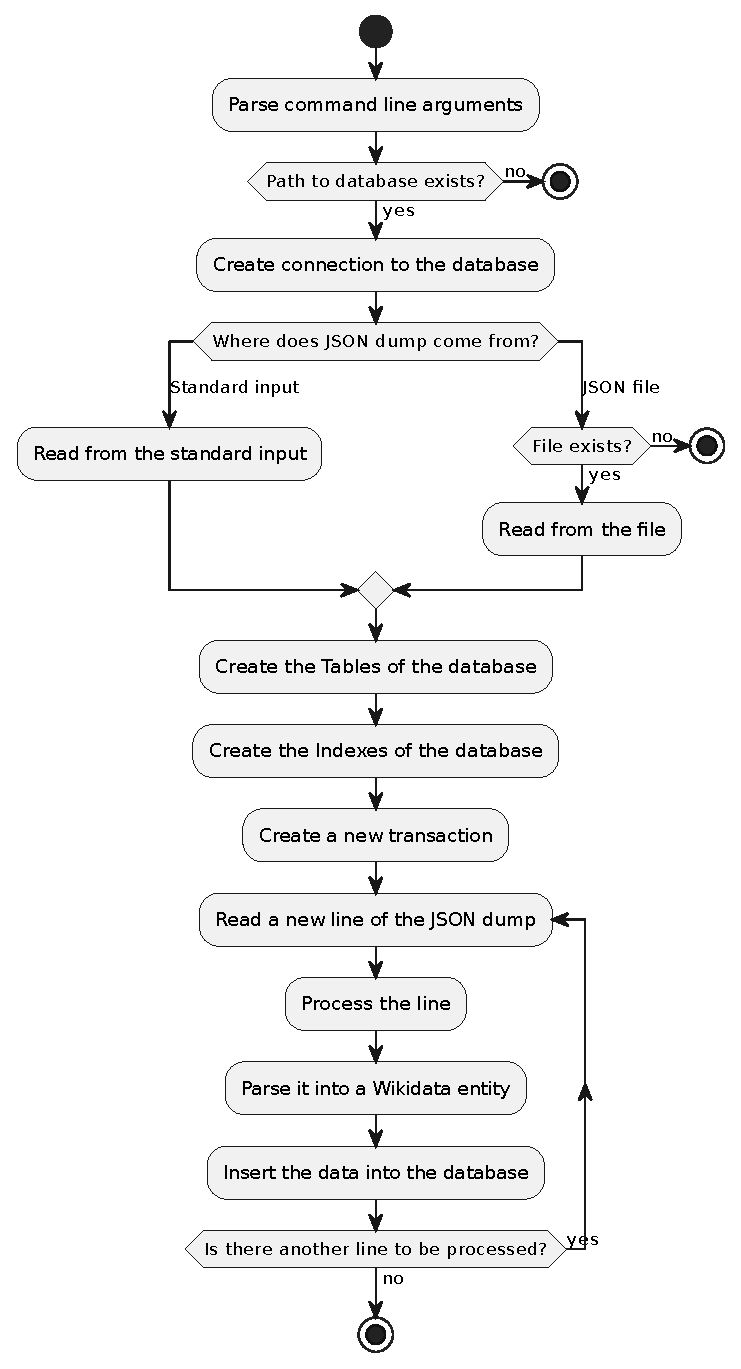
\includegraphics[width=.66\linewidth]{figures/diagrams/10-2_wd2duckdb.pdf}
    \caption{Activity diagram of the \texttt{wd2duckdb} tool}
    \label{fig:activity}
\end{figure}%

\label{section:optimizations}
\subsection{Optimizations}

The Wikidata JSON dump is a huge file. As we have seen in section \ref{section:issue}, it is around \texttt{1.5 TB} in size. This means that we need to put an extra effort into optimizing the tool. For that, we are going to use a combination of different techniques, such as compression, and fine-tuning the chosen data types.

\subsubsection{Compression}

Dealing with large amounts of data is far from being trivial. For that, we are going to use compression techniques to reduce the size of the data that we are going to store. Those mechanisms can potentially reduce the size of the data by a factor of 10. This is not only beneficial for reducing the storage footprint, but it also helps improve the performance of tools consuming the data as fewer reads from disk or over a network connection are required. Column store formats are known for being highly compressible, and DuckDB is not an exception. This is because data within a column tends to be similar to each other, which is not the case for row-based formats, where each row is composed of heterogeneous data types, leading to lower compression rates.

The best thing about compression in DuckDB is that it will automatically choose the better compression algorithm for us \cite{Raasveldt_2022}. This is because it can detect the data type of each column, and based on that, it will choose the best compression method. For example, DuckDB will probably choose \texttt{RLE or Run-length encoding} for storing the identifiers of the properties, as it decomposes the dataset into pairs of (value, count) tuples, where the count represents how many times the value is repeated. Thus, no repeated values are stored. This is useful as several different entities may claim the same property, such as \texttt{P31} (instance of), where almost every Wikidata item will have it. Hence, we can take advantage of this and compress the data using \texttt{RLE}. To put it in a nutshell, \texttt{RLE} is a lossless compression algorithm that replaces repeated values with a single value and a count. This is illustrated in figure \ref{fig:rle}.

\begin{figure}[ht]
    \centering
    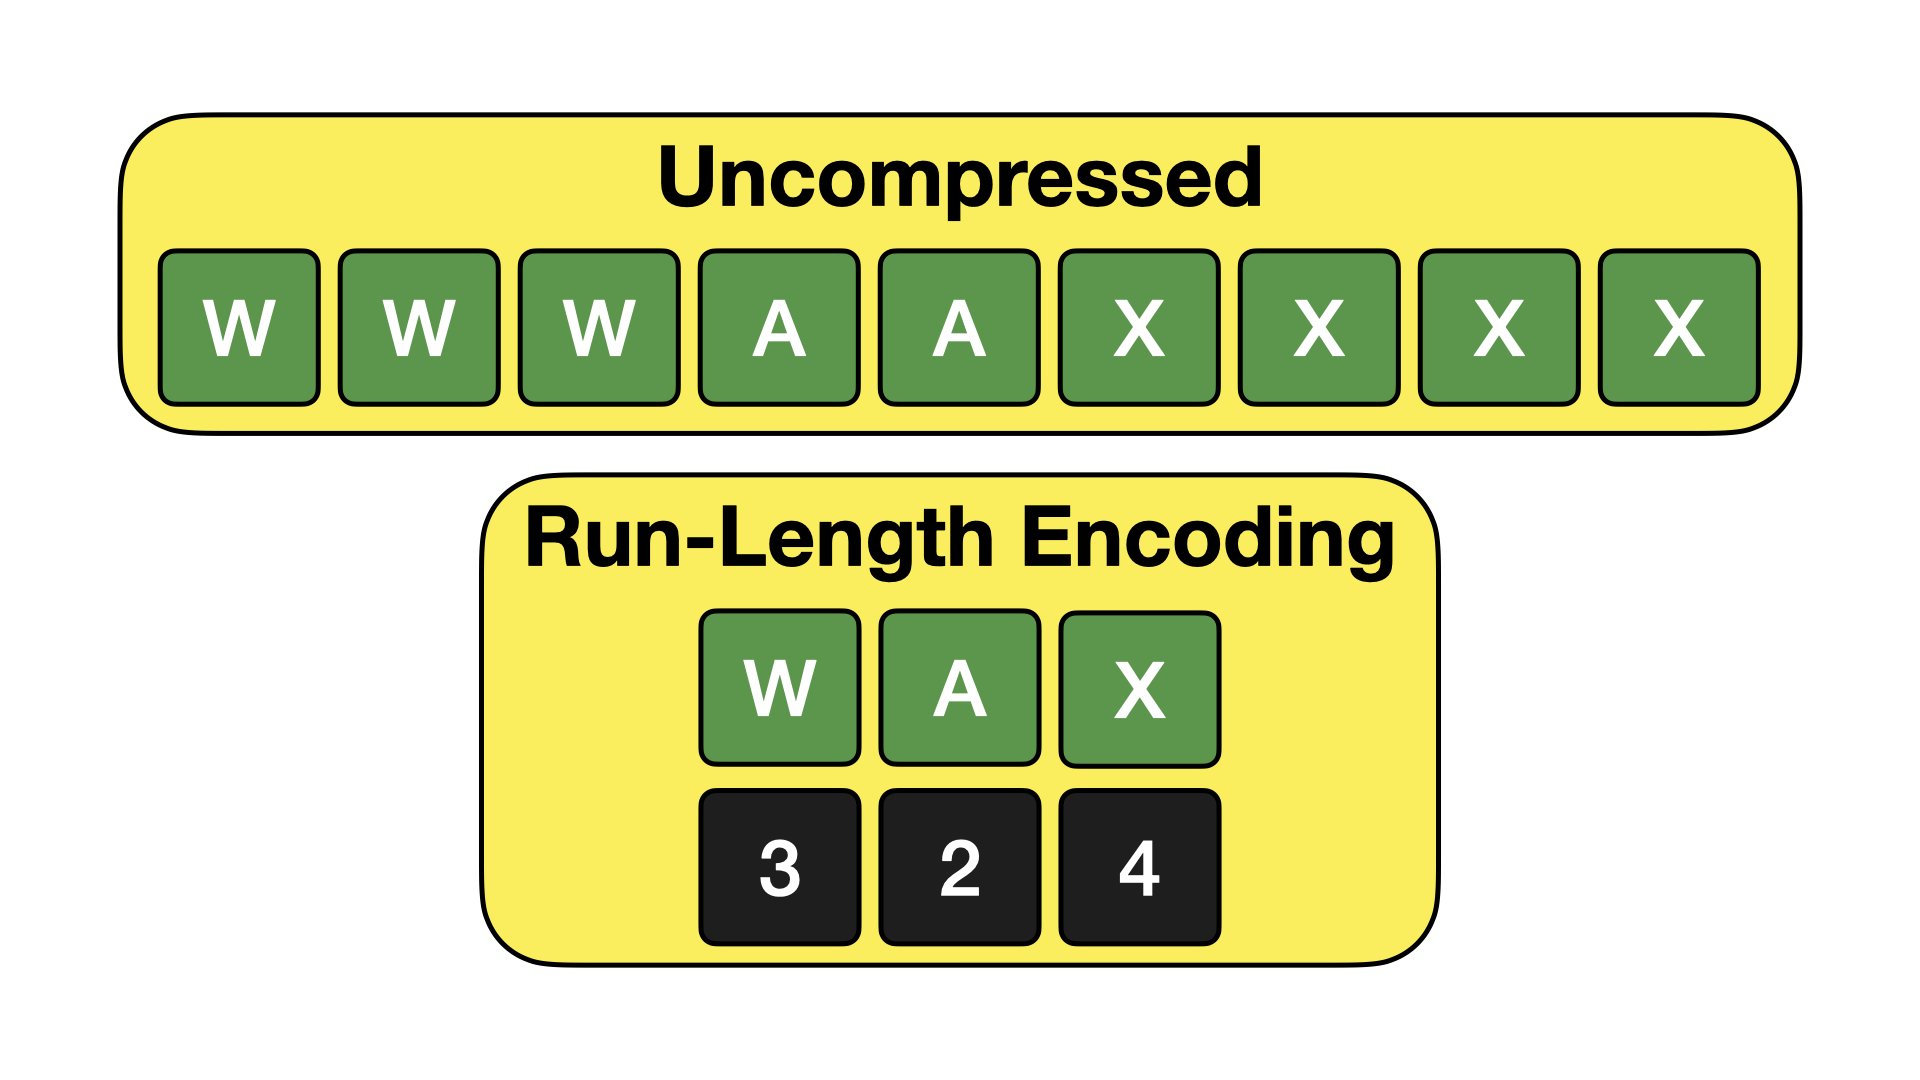
\includegraphics[width=.8\linewidth]{figures/diagrams/10-2_rle.png}
    \caption[Example of \texttt{RLE} compression]{Example of \texttt{RLE} compression \cite{Raasveldt_2022}}
    \label{fig:rle}
\end{figure}

In the given example, the original sequence \texttt{WWWAAXXXX} is compressed into \texttt{3W2A4X}. This transformation is achieved by identifying repeated characters, such as the \texttt{W} occurring thrice, the \texttt{A} occurring twice, and the \texttt{X} occurring four times. Thus, we can replace the repeated values with a single value and a count. The \textit{run-length encoding} preserves the same information as the original sequence but in a more concise format. Additionally, we have successfully represented the initial string, consisting of nine characters, with a string of only six characters, resulting in a 33\% reduction in size. It is worth noting that the compression rate improves as the number of repetitions increases. Although this example is straightforward, it effectively demonstrates the underlying concept of \texttt{RLE}.

Another possibility is \texttt{FSST or Fast Random Access String} for compressing \texttt{STRING} columns. This mechanism aims for creating a dictionary of references and segments which are repeated across the dataset. This is effective when dealing with unique strings, such as \textit{labels} or \textit{descriptions} in our case, having plenty of repetitions within them. For example, descriptions of entities from the same real-world domain may contain repeated words, such as in the case of \texttt{Q2} (Earth) or \texttt{Q193} (Saturn), where the word \texttt{planet} may appear several times. Thus, we can take advantage of this, and compress the data using the \texttt{FSST} algorithm. The way it works is by creating a \textit{symbol table} that maps each unique string to an integer identifier. Then, the original string is replaced by the corresponding identifier. This is illustrated in figure \ref{fig:fsst}.

\begin{figure}[ht]
    \centering
    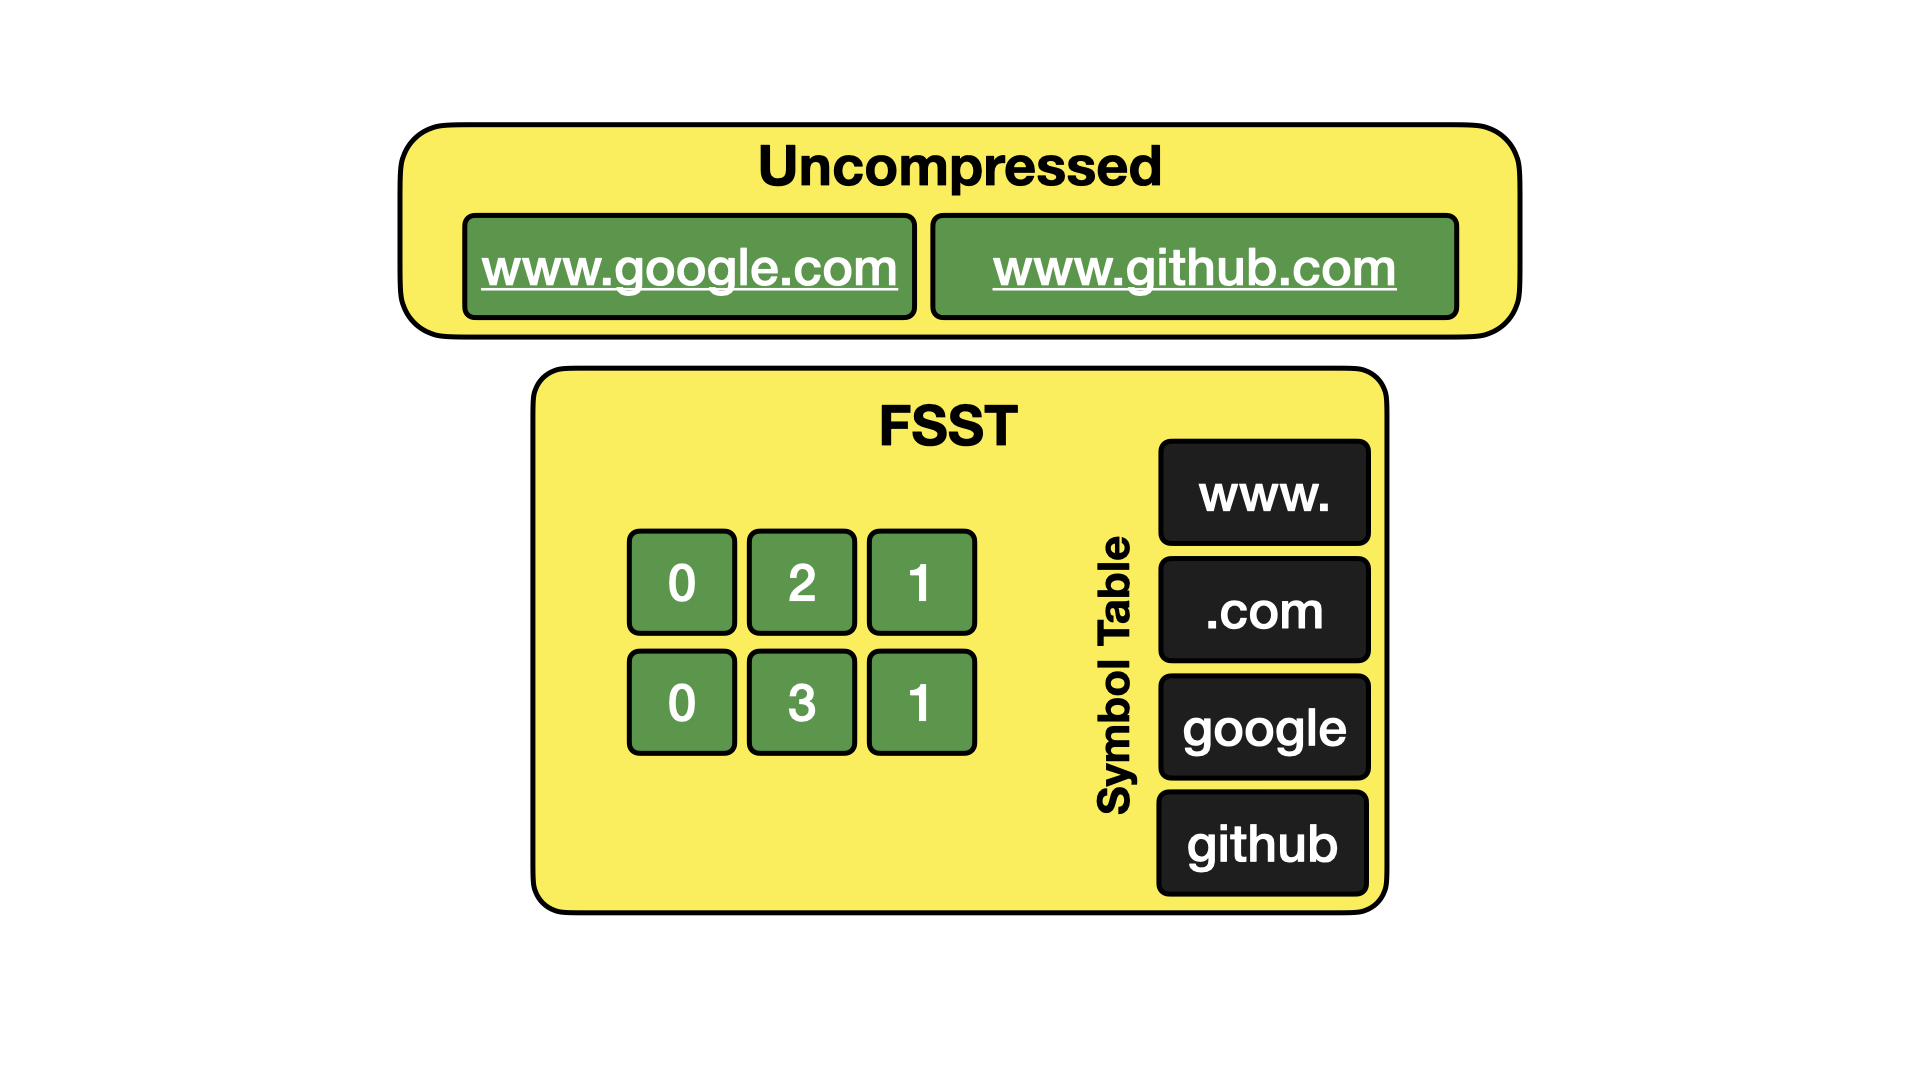
\includegraphics[width=.8\linewidth]{figures/diagrams/10-3_fsst.png}
    \caption[Example of \texttt{FSST} compression]{Example of \texttt{FSST} compression \cite{Raasveldt_2022}}
    \label{fig:fsst}
\end{figure}

Note that in the previous example, the original sequence \texttt{www.google.com} is compressed as \texttt{021}. Where \texttt{0} is the identifier for \texttt{www.}, \texttt{2} identifies \texttt{google} and \texttt{1} stands for \texttt{.com}. As in the case of \textit{run-length encoding} the higher the number of repetitions, the higher the level of compression. In this case, we have successfully represented the initial string, consisting of 14 characters, with a string of only three characters, resulting in a 78\% reduction in size. Although this example is straightforward, it effectively demonstrates the underlying concept of \texttt{FSST}.

One of the greatest strengths of compression in columnar storage lies in the driver's ability to select the optimal algorithm for each scenario. Specifically, in a column-oriented store, we can leverage a variety of compression mechanisms, individually tailored to excel in compressing each column, given that we are dealing with homogeneous data. Conversely, row-oriented stores limit us to a single compression algorithm for the entire dataset. This limitation arises from the heterogeneity of the data, preventing us from employing distinct compression algorithms for each column.

\subsubsection{Data types}

According to what we have seen in the introductory lines, we are going to try and optimize as much as we can the data types that we are going to use for storing the information. For that, we are going to use the smallest data type that can hold the information we are interested in. For example, we are using \texttt{UINTEGER} for storing the IDs of the entities, as they can be represented as numbers. What's more, we are going to use the unsigned representation as we are not interested in negative numbers. This has two main benefits: first, we are going to be able to store larger numbers. To put it into perspective, the maximum value range that can be stored in a \texttt{UINTEGER} is \texttt{4,294,967,295}, whereas the largest number that can be stored in an \texttt{INTEGER} is \texttt{2,147,483,647}. This means that we can handle twice as many positive values with the same number of bits. The same reasoning applies to the rest of the data types that are going to be used. Second, we ensuring e that our data is consistent. This is, we are not going to be able to store negative numbers in a column that is supposed to store positive numbers.

From my perspective, fine-tuning the chosen data types for storing your data makes your repositories more robust. This is because you are ensuring that the data that you are working with is consistent and that you are not wasting any space. This is especially important when dealing with large amounts of data, as the storage footprint can be reduced by a factor of 2. This is the case for this project. At the beginning of it, we were using \texttt{BIGINT} for storing the IDs of the entities. However, we realized that we were wasting half of the space, as the IDs are always positive. For that, we decided to switch to \texttt{UINTEGER}. Summing up, we moved from an 8-byte integer to a 4-byte representation, which means that we were able to store twice as many IDs with the same number of bits. This also leads to fitting more data both in memory and in the cache, which is going to be beneficial for the second part of the tool, where the graph is going to be built.

Regarding the encoding of IDs, we had two main possibilities. First, we could have used the string representation, which is the one that is employed in the JSON dump. However, we decided to go for the numeric representation as it is more compact. This is because the string representation of the IDs is composed of a prefix followed by a sequence of numbers. For example, the string representation of the ID \texttt{Q92743} is \texttt{"Q92743"}, whereas the numeric representation of the same ID is \texttt{92743}. As we are using a \texttt{UINTEGER} for representing the numeric data, only 4 bytes per row are needed. However, a string takes 1 byte per character. Thus, according to the previous example, we would need 6 bytes for encoding the string representation of the ID, while only 4 are required for the numeric representation. In this example, 2 bytes are saved. Note that this scales for even larger IDs.

The problem is that things are not as simple as they seem at first glance. Wikidata IDs not only are numeric identifiers, but they also annotate the type of the item they support: Entities, Properties, Lexemes, Forms and Senses. Thus, we need a way for encoding and decoding this information. For this purpose, what we have done is diving the address space of the IDs into 5 different ranges, one for each type. The ranges have a length of 1 hundred million, except for Forms and Senses, each of them has half that size, which is more than enough for representing the different Wikidata IDs. See the code below for more information.

\begin{code}[The From trait implementation for the ID type]
    \inputminted{rust}{code/listings/10-1_ids.rs}
\end{code}

It is worth mentioning that the most powerful thing about the \texttt{From} \texttt{trait} in Rust is that it allows us to not only convert from one type to another; but in the opposite direction too. This is, it automatically implements the \texttt{Into} \texttt{trait} thanks to the blanket implementation in the standard library. Hence, now we can convert from \texttt{u32} to \texttt{Id} and vice-versa. That is, we can serialize and deserialize the IDs transparently.

\subsubsection{Memory allocator}

A memory allocator is a software component that manages the allocation and deallocation of memory in a program. Its primary goal is to efficiently use available memory by keeping track of allocated and free memory blocks. Allocators work with a memory region called the heap, where objects are dynamically allocated. When a program requests memory, the allocator finds a free block, marks it as allocated, and returns a pointer to the program. Deallocation involves marking the block as free.

Memory allocators can employ various algorithms and data structures to manage memory efficiently. They may use techniques like linked lists, bitmaps, or binary trees to track the state of memory blocks and quickly find free blocks for allocation. Additionally, advanced allocators may employ strategies like caching, thread-specific allocation pools, or memory reuse techniques to optimize performance and reduce overhead.

Different programming languages and platforms often provide default memory allocators, but developers can also choose alternative allocators, such as \texttt{Jemalloc}, for specific optimizations or requirements. By selecting an appropriate memory allocator, developers can improve memory usage, minimize fragmentation, enhance performance, and cater to the specific needs of their applications.

\texttt{Jemalloc} is a memory allocator that can be used in Rust binary projects to optimize memory management and improve application performance. When a program allocates and deallocates memory frequently, the default memory allocator in Rust (system allocator) can introduce overhead due to its design choices and trade-offs, as it is optimized for general-purpose use and targets several different platforms and environments. However, \texttt{Jemalloc} is a specialized allocator that aims for reducing memory fragmentation. When memory allocation and deallocation are frequent, small gaps tend to form between allocated memory blocks. These gaps are called fragmentation and can lead to inefficient memory usage. Note that in the context of Big data applications, efficient memory management may improve the performance of the solution by orders of magnitude. \texttt{Jemalloc} uses a technique called \textit{arena-based memory allocation} to reduce fragmentation and improve performance. It also uses a \textit{thread-specific caching} strategy to reduce the overhead of synchronization and improve performance in multi-threaded applications. As we will see in the next chapter, one of the main optimizations that we will implement is writing our solution in a multi-threaded fashion. Thus, using \texttt{Jemalloc} is going to be beneficial for us. Lastly, note that \texttt{Jemalloc} is a platform-specific allocator, which means that it is only available on Linux and macOS. However, this allows it to use platform-specific features to improve performance.

For us to use \texttt{Jemalloc}, we need to add the following lines to the \texttt{Cargo.toml} file.

\begin{code}[The Cargo.toml file for using Jemalloc]
    \inputminted{toml}{code/listings/10-2_cargo.toml}
\end{code}

What's more, we need to use it as the default allocator for our application. For this, we need to add the following lines to the \texttt{main.rs} file. Recall that the memory allocator should be set in the main function of the application before any other code is executed. This is because the allocator is a global resource, and it is not possible to change it once it has been set. Note that in the case of libraries, changing the allocator won't have any impact, as it is the responsibility of the application to do so.

\begin{code}[The main.rs file for using Jemalloc]
    \inputminted{rust}{code/listings/10-3_main.rs}
\end{code}

\subsubsection{Compiler options}

During the development stage, Rust applications are constructed using the \texttt{dev} flag, which compiles the program without applying any optimizations. By default, the \texttt{opt-level} is set to 0 in order to facilitate easy debugging. The compilation process focuses on detecting potential panics or errors during execution. However, when preparing the tool for deployment, it is recommended to utilize the \texttt{release} profile, which leverages maximum optimization. The \texttt{opt-level} is set to 3 by default, enabling beneficial optimizations. Functions are rewritten to execute faster, incorporating techniques like inlining that make them harder to debug. Additionally, the \texttt{LTO} (Link Time Optimization) is enabled, allowing the compiler to optimize code across different compilation units. This is particularly significant when working with various modules and crates. By utilizing the \texttt{LTO} build, we aim to discover optimizations that span across different dependencies and crates, although this may result in slower compilation times. The \texttt{Cargo.toml} file specifies the release profile as follows:

\begin{code}[The Cargo.toml file for using the release profile]
    \inputminted{toml}{code/listings/10-4_cargo.toml}
\end{code}

\subsubsection{Targeting the right Platform}

Targeting the right platform in Rust is essential for optimizing performance. By specifically focusing on the platform, you can leverage architecture-specific optimizations, taking advantage of specialized hardware accelerators and maximizing the efficiency of memory management. Rust's compiler offers optimization flags and the ability to link with platform-specific libraries, enabling tailored performance enhancements. This approach ensures compatibility with the target platform's operating system, architecture, and hardware configurations, ultimately resulting in improved performance and efficiency for Rust applications. For us to target the right platform, we need to add the following lines to the \texttt{.cargo/config} file.

\begin{code}[The .cargo/config file for targeting the right platform]
    \inputminted{toml}{code/listings/10-5_config}
\end{code}

\subsection{Quality assurance}

In the following subsections, we are going to discuss the different quality assurance mechanisms that are going to be used for the development of the tool. The idea is to ensure that it is robust and that can be used in production environments. For that, we are going to use a combination of different techniques, such as version control, documentation, testing, continuous integration and continuous deployment. Note that the tool is going to be open-source, which means that the community will be able to contribute to the project. This is going to be beneficial for it as it will allow us to build a more robust tool, as third parties can examine the product we ship. Lastly, note that we are going to use this same methodology for the development of the other tools that are going developed in this thesis.

\subsubsection{Version control}

Recall that we are building an open-source solution. For this, we are going to use Git as our version control system. The idea is to use GitHub as our remote repository. This will allow us to have a public warehouse where the community can contribute to the project. Moreover, we are going to use Git tags for the versioning, letting us have a clear understanding of the different versions of the tool. For instance, we are using the \texttt{v0.0.1} tag for the first version. Subsequent versions will be annotated with a \texttt{v0.0.x} tag. What's more, for the sake of simplicity, we are going to use \textit{stable mainline} as our branching strategy for the development of the tool. This means that we are going to have a \texttt{main} branch where the latest stable version is going to be stored. The idea is to have a \texttt{dev} branch where most of the development process is going to take place. Once we have a stable version, we will merge it into the \texttt{main} branch. Note that this is a simple branching strategy that will work just fine for the development of this project as I am the sole developer. However, for larger projects, a more complex branching strategy should be considered.

\subsubsection{Documentation}

Having that said, writing good documentation is essential for the development of a robust project. For that, we are going to use Rust's documentation tool, namely, \texttt{rustdoc}. The idea is to document the different \texttt{functions}, \texttt{structs}, \texttt{traits} and \texttt{modules} of the tool so that the community can have a clear understanding of its API. Moreover, we are going to use \texttt{rustdoc}'s \texttt{doc-tests} feature for writing tests in the documentation. Putting this all together, the whole documentation will be deployed to \texttt{docs-rs}\footnote{\url{https://docs.rs/wikidata-rs/latest/wikidata_rs/}}.

\subsubsection{Testing}

The idea is to have a robust tool that can be used in production environments. For that, we are going to use Rust's testing framework, namely, \texttt{cargo test}. The idea is to write unit tests for the different functions of the tool. Something neat about \textit{unit testing} in Rust is that it encourages developers to write tests in the same file\footnote{\url{https://github.com/angelip2303/pregel-rs/blob/main/src/pregel.rs\#L873}} as the code. This is a good practice as it allows us to have a clear understanding of the different tests that are being run.

\subsubsection{Continuous integration and continuous deployment}

The result of combining the previous techniques is a robust tool that can be used in production environments. However, we are going to take it one step further by using continuous integration and continuous deployment. The idea is to make use of GitHub Actions. This is, having an Action that will run the tests of the tool every time a new commit is pushed to the repository's \texttt{main} branch. This will allow us to have a clear understanding of the state of the tool. Moreover, we are going to have another GitHub Action that will be in charge of deploying the tool to the \texttt{crates.io}\footnote{\url{https://crates.io}} platform so that other developers can use it in their projects.

\subsection{User manual}

\subsubsection{Installation}

Make sure that you install the latest stable version of Rust\footnote{\url{https://www.rust-lang.org/}}; that is, as of May 5th, version 1.69 or later, then run:

\begin{minted}{shell-session}
$ cargo install wd2duckdb
\end{minted}

This will compile \texttt{wd2duckdb} for your native architecture, increasing the performance. Recall the optimizations that we have discussed in the previous section. However, if you want to compile it for a different architecture, you can use the \texttt{--target} flag.

\subsubsection{Usage}

Several command-line options are available to customize the behavior of \texttt{wd2duckdb}. The following is a list of the most important ones:

\begin{enumerate}
    \item \texttt{--json}: The path to the \texttt{.json} file that contains the Wikidata dump. This is a required argument.
    \item \texttt{--database}: The path to the DuckDB database file. This is a required argument.
\end{enumerate}

The following is an example of how to use the tool:

\begin{minted}{shell-session}
$ wd2duckdb --json <JSON_FILE> --database <DUCKDB_FILE>
\end{minted}

Use \texttt{-} as \texttt{<JSON\_FILE>} to read from standard input instead of from a file. This makes it possible to build a pipeline that processes JSON data as it is being decompressed, without having to decompress the full dump to disk. In the case of a \texttt{.bz2} file, you can use the following instruction:

\begin{minted}{shell-session}
$ bzcat latest-all.json.bz2 | wd2duckdb --json - --database <DUCKDB_FILE>
\end{minted}

In case of a \texttt{.gz} compressed file, the following is required:

\begin{minted}{shell-session}
$ gunzip latest-all.json.gz | wd2duckdb --json - --database <DUCKDB_FILE>
\end{minted}

In case you want to write changes directly to the standard output; that is, without creating a file for the uncompressed \texttt{.json}, you can do the following. Note the use of the \texttt{-c} flag in \texttt{gunzip}:

\begin{minted}{shell-session}
$ gunzip -c latest-all.json.gz | wd2duckdb --json - --database <DUCKDB_FILE>
\end{minted}

If you are working with large dumps where the uncompressed \texttt{.json} file size is in the order of \texttt{Terabytes}, it is best to choose the last option. The \texttt{.duckdb} file, which is more memory-efficient, may thus be created immediately. This is because the \texttt{.json} file is not stored in memory, but rather, it is streamed from the standard input.

\subsection{Known limitations}

During the development of our tool, we encountered a limitation related to the \texttt{wikidata}\footnote{\url{https://crates.io/crates/wikidata}} library, which cannot parse JSON dumps before 2017-08-21. This limitation is shared by other tools aiming to import Wikidata dumps\footnote{\url{https://github.com/usc-isi-i2/kgtk/issues/108}}, as mentioned in an issue reported on GitHub. Although the specific reasons for this limitation are not well-documented in Wikidata's developer portal, we have found some clues that may provide insights into the possible cause\footnote{\url{https://github.com/usc-isi-i2/kgtk/issues/272\#issuecomment-748350311}}. The limitation arises from the way references to properties and values are serialized in the dumps. Recall figure \ref{fig:wikibaseStatement}, where we can see that the Statement has a \texttt{mainSnak}, which is the main claim of the statement. Before the mentioned date, the referencing was done using only the numeric identifier (\texttt{numeric-id}) instead of the full identifier expected by the library. For example, the property \texttt{P31} was referenced as \texttt{\{numeric-id: 31\}} instead of \texttt{\{numeric-id: 31, id: "P31"\}}. Hence, the library fails to parse the Wikidata entities. Even if we will continue monitoring the development of the \texttt{wikidata} library to see if this issue is resolved in future updates, fixing it ourselves is challenging and not a priority for our tool's development at the moment, as we can work with dumps from 2017-08-21 onwards.

\chapter{A tool for validating Knowledge Graphs}
\label{chapter:pschema}
\epigraph{\textit{Logic is the foundation of the certainty of all the Knowledge we acquire.}}{-- \textup{Leonhard Euler}}

As we have seen thus far, the thesis' main goal is to create a tool capable of creating subsets out of a Knowledge Graph provided a \texttt{Shape Expression} schema. To achieve so, in this chapter, we will explore two main ideas. Firstly, we will comment on the possibility of implementing the Pregel framework in Rust. Secondly, we will design a tool for validating a Knowledge Graph against a \texttt{Shape Expression}, following a novel approach.

\section{Pregel-rs}

The \texttt{pregel-rs} library is a Rust fork of the original Pregel framework that we have already discussed in chapter \ref{chapter:theory}. This library is available on GitHub\footnote{\url{https://github.com/angelip2303/pregel-rs}}.

\subsection{Design}

Long has been discussed about the Pregel framework, thus far. However, for us to implement it, we need to make certain design decisions. This section will outline the compromises we have made to successfully implement it in Rust.

First and foremost, it should be acknowledged that when transitioning from the Scala-based solution to the Rust-based one, we were fully aware that building the solution on top of existing projects would not be feasible. Rust, being a relatively new language, is not as mature as Java. Consequently, certain features would need to be developed from scratch. Thus, we started the development of the Pregel library, which will be utilized to implement the subgraph matching algorithm.

It is important to note that we have deliberately separated the framework from the algorithm implementation addressed in this thesis. This decision was made to maximize the framework's flexibility. By adopting this approach, not only can we utilize the framework in other projects, but we can also extend its capabilities to support additional features. To put an example, we have successfully incorporated the \textit{PageRank} algorithm into the framework as an additional feature to demonstrate its versatility. In the following sections, we will discuss the design and implementation details of the Pregel library.

\label{section:pregel-rs}
\subsubsection{The \texttt{pregel-rs} library}

Recall that Rust is heavily oriented to be executed in single machines. This means that we won't use the Pregel framework to process graphs in a distributed manner. Instead, we will use it to process graphs in a \textit{centralized system}. Back when the Pregel framework was introduced, the hardware resources available for single-node systems were limited. However, nowadays, we can leverage the benefits of multi-core processors to process graphs in a centralized manner. Thus we will make use of techniques such as \textit{multi-threading} to process graphs in a single machine. Note that the creation of the \texttt{wd2duckdb} tool was motivated by the idea of trying to make it fit the whole graph in memory. To put it into perspective, as of 2023, we, as customers, can purchase a memory module with a capacity of 128 GB with a total cost of $\$269.90$. However, this was not the case back in 2010, when the Pregel framework was introduced. Thus, we are hopeful that we can create a Pregel-like framework that instead of processing graphs in a distributed manner, can make use of the hardware resources available in a single machine; this is, a \textit{multi-threaded Pregel}. Recall what we have mentioned in section \ref{section:rust} about the way \textit{concurrency and parallelism} are implemented in Rust.

The idea then is to optimize the use of memory as much as we can to process graphs in a single machine. As a comparison, the size of the Wikidata JSON dump created as of August the $21^{th}$ 2017 is 16.94 GB compressed (224.42 GB uncompressed), while the \texttt{.duckdb} database file created by the \texttt{wd2duckdb} tool is 9.38 GB. This means that we can fit the whole graph in memory, and hence, we can fit the graph in a single machine. However, we need to be careful when processing the graph, as we can easily run out of memory by annotating it with additional information. To avoid this, we will make use of the \textit{lazy evaluation} technique. This mechanism will allow us to process the graph in a \textit{streaming} manner, which will reduce the memory footprint of the application. More into this will be discussed later on.

Firstly, we are describing the series of steps that the Pregel framework follows to process a graph. This sequence is depicted in figure \ref{fig:sequence}. The execution starts by sending the initial messages to the vertices at iteration 0. Then, the first -- actual -- \textit{superstep} begins. This loop will last until the current iteration is greater than the threshold set at the creation of the Pregel instance. At each iteration, the vertices will send messages to their neighbors, provided the given direction, and subsequently, they may receive messages sent from other nodes. Moving forward, an aggregation function is applied, and the vertices are updated accordingly. Finally, the iteration counter is incremented, and the next iteration starts until the threshold is reached.

\begin{figure}[ht]
    \centering
    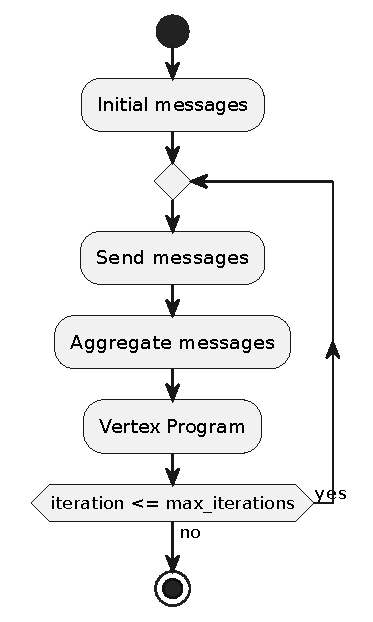
\includegraphics[width=0.4\textwidth]{diagrams/11-1_pregel.pdf}
    \caption{The Pregel framework as implemented in \texttt{pregel-rs}}
    \label{fig:sequence}
\end{figure}

As you can observe, the described process is far from being complex. Thus, we can agree that the Pregel framework is a simple abstraction for graph processing. However, this simplicity is what makes the Pregel paradigm so powerful. By abstracting the underlying model, we can focus on the problem at hand, rather than the implementation details of the framework. By doing so, we can focus on the implementation of the \textit{subgraph matching algorithm}, rather than the implementation details of the Pregel model itself. Now that we have a better understanding of what we are trying to build, we can move forward and discuss some of the design decisions we have made.

\subsubsection{The Builder pattern}

In Rust, there is no direct support for constructors. Instead, the convention is to use an associated function called \texttt{new} that returns an instance of the \texttt{struct}. However, this restricts the creation of objects to only one possible representation, since multiple functions cannot have the same identifier. Unlike Java, where we can have multiple constructors with the same name, as long as they have different parameters. To overcome this limitation and enable the creation of different representations of the same object, we can use the \textit{Builder pattern}.

\begin{figure}[ht]
    \centering
    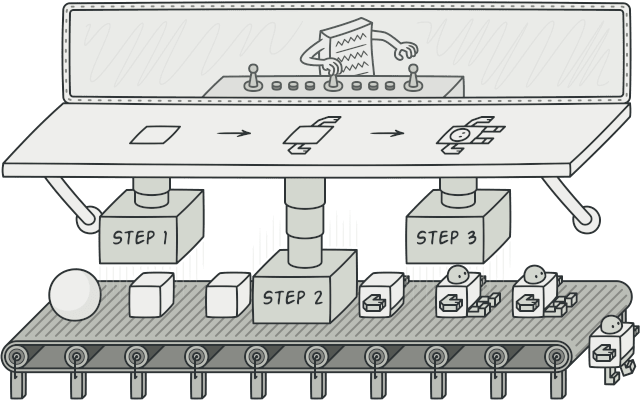
\includegraphics[width=0.66\textwidth]{diagrams/11-2_builder.png}
    \caption[Diagram showing the idea behind the \textit{Builder pattern}]{Diagram showing the idea behind the \textit{Builder pattern}\footnotemark}
\end{figure}
\footnotetext{\url{https://refactoring.guru/design-patterns/builder}}

This is a creational design pattern that allows us to decouple the construction of a complex object from its functionality. By separating the construction process, we gain the flexibility to create diverse representations of the object itself. This pattern effectively resolves the issue of dealing with constructors that have an excessive number of parameters and also addresses Rust's limitation of having only one \texttt{new} function per \texttt{struct}. It also allows us to \textit{create} objects in a -- somewhat -- functional manner, which is a common practice in Rust. As a last remark, the \textit{Builder pattern} allows us to create a default representation of the object, which is useful when we want to create a default configuration of it, and then modify it accordingly. What's more, it allows us to build objects in such a manner that some configuration aspects are optional. In the example below we can observe the creation of a Pregel instance using the Builder pattern. What we are doing is creating a default configuration of the Pregel instance, by calling the \textit{new} function, passing the \texttt{GraphFrame} object, which is the only required parameter. Then, by subsequent calls to the builder methods we can modify the object's representation. As an example, we are setting the maximum number of iterations to 4. Finally, we are calling the \texttt{build} function which will return the -- actual -- Pregel instance with the desired representation. Note that, in this case, what we are building is the so-called \textit{PageRank} algorithm\footnote{\url{https://github.com/angelip2303/pregel-rs/blob/main/examples/pagerank.rs}}, which is a well-known algorithm for ranking web pages.

\begin{code}[Creating a Pregel instance using the Builder pattern]
    \inputminted{rust}{code/listings/11-3_pagerank.rs}
\end{code}

\vspace*{1em}

\subsection{Implementation}

We will now discuss the implementation details of the Pregel library that we have just described. Recall that we are willing to create a tool that is implemented on top of a DataFrame API, as we want to leverage the benefits of this abstraction that we have already discussed in chapter \ref{chapter:refactoring}. Thus, we will now comment on the implementation details of the Pregel library.

\subsubsection{The \texttt{GraphFrame} struct}

The first step is to create a representation of the graph that we are going to process. To do so, we have created the \texttt{GraphFrame} struct. This struct is a wrapper around the \texttt{pola-rs} \texttt{DataFrame} library, which is the equivalent in Rust to Apache Spark's \texttt{DataFrame API}, as we have seen in chapter \ref{chapter:analysis}. This \texttt{struct} is responsible for storing the graph's vertices and edges, as well as extending its basic functionality to support some useful operations. For example, we have implemented the \texttt{from\_edges} function, which is responsible for creating a \texttt{GraphFrame} instance from a set of edges. This function is useful since it allows us the creation of the \texttt{GraphFrame} from the entities that we have extracted from the Wikidata JSON dump in chapter \ref{chapter:wd2duckdb}.

As we have introduced in section \ref{section:pregel-rs}, the way we are implementing the \texttt{pregel-rs} library is through a \texttt{Lazy API}\footnote{\url{https://pola-rs.github.io/polars-book/user-guide/concepts/lazy-vs-eager/}}. What we mean by this is that operations are not computed until we explicitly specify so. This has a great advantage when working with large datasets, as we can \textit{optimize} the query we are building. Let me clarify this. When we evaluate functions more traditionally; that is, \textit{eager evaluation}, expressions are computed as soon as they are defined. This means that, if we have a chain of operations, each operation will be computed as they appear in the code. However, things are different when using \textit{lazy evaluation}, as expressions are not computed until we need the actual result of the evaluation. This allows \textit{query engines} to optimize\footnote{\url{https://pola-rs.github.io/polars-book/user-guide/lazy/optimizations/}} the query, by reordering the operations in such a way that the number of actual computations is reduced. In the example below, we can observe how operations are not computed until we call the \texttt{collect} function, in line 20, which is the one that triggers the computation. Note that we can use this technique as we call the \texttt{lazy} function before referring to the computations we want to perform over the dataset. This has another enormous advantage, which is that we can \texttt{clone} the objects that we are working with, without having to worry about the performance implications of doing so. This is because, as we have mentioned, the actual computation is not yet performed, and hence, we are just \texttt{cloning} the \textit{query plan}\footnote{\url{https://stackoverflow.com/questions/72320911/how-to-avoid-deep-copy-when-using-groupby-in-polars-rust}}.

\begin{code}[GraphFrame implementation in \texttt{pregel-rs}]
    \inputminted{rust}{code/listings/11-1_graph.rs}
\end{code}

\vspace*{1em}

\subsubsection{The \texttt{Pregel} framework}

Thus far, quite a lot has been said about different \texttt{structs} and features that are helpful for the implementation of the Pregel algorithm. However, we have not yet discussed the actual algorithm. In this section, we will comment on the implementation details of the Pregel model in Rust, which is the core of the \texttt{pregel-rs} library. Recall diagram \ref{fig:sequence} where we showed the different steps that are involved in the Pregel framework.

First, we will start by describing the \texttt{initial\_message} step\footnote{\url{https://github.com/angelip2303/pregel-rs/blob/main/src/pregel.rs\#L764}}. Note that, at this point, we are working with a Graph containing a bunch of vertices and edges. No operation has been performed yet. Thus, we need to create -- at least -- one extra column for the messages to be sent, back and forth. What's more, we have to initialize that column to a certain value, which is specified by the user during the configuration of the Pregel instance. Regarding the point in time at which we \texttt{collect} the results of the computation, this will be performed at the end of each \textit{superstep}. This means that, at the end of each iteration, we will get a DataFrame containing the vertices having the different operations evaluated. By doing this, we ensure that at the beginning of each iteration, the vertices are in the state that we expect them to be. Recall that in the Pregel model, the \texttt{initial\_message} step is known as the \textit{superstep 0}, and hence, we will \texttt{collect} the results of the computation.

Note that another optimization is introduced here, which is the use of the \texttt{Streaming API}\footnote{\url{https://pola-rs.github.io/polars-book/user-guide/lazy/streaming/}}. With the combination of the \texttt{lazy} and \texttt{streaming} APIs, we can perform the computation in such a way that we are not going to load the whole dataset into memory, but it is going to be processed in chunks. This is a great advantage when working with large datasets, as we can avoid the \textit{out of memory} errors that we would otherwise encounter. Another advantage is that we can work with datasets that are larger than RAM. See the code below for a more detailed explanation.

\begin{code}[Initial Message step as implemented in \texttt{pregel-rs}]
    \inputminted{rust}{code/listings/11-4_initial.rs}
\end{code}

To go a step further, we will now describe the main loop of the Pregel algorithm. This is, we now have all the vertices and edges of the Graph annotated with an extra column, namely, the \texttt{vertex\_column}. Thus, it is time for the \textit{superstep 1} to begin. This is divided into three main pieces. The first step is to send the messages in the appropriate direction. Just after that, those messages are aggregated. Lastly, the vertices are updated accordingly. For us to perform the first step, we must apply the \texttt{send\_message} function to the whole graph. After that, the messages are going to be sent in the given direction. Note that, one node may have many neighbors. Hence, we must \textit{aggregate} the messages into a single one. This is done by applying the \texttt{aggregate\_messages} function. In the case of the \texttt{pregel-rs} library, we are using a \texttt{groupby} context. The code below shows how it is implemented\footnote{\url{https://github.com/angelip2303/pregel-rs/blob/main/src/pregel.rs\#L829}}. Note that some simplifications have been made, but the idea is the same.

\begin{code}[Send and Aggregate Messages step as implemented in \texttt{pregel-rs}]
    \inputminted{rust}{code/listings/11-5_msgs.rs}
\end{code}

Moving on, now that we have the messages sent and properly aggregated, it is time to update the vertices. What we mean by this is that according to the Pregel model, the vertices may need to be modified to reflect their new state due to the messages they have received. This is done by applying the \texttt{v\_prog} function to the graph. For us to achieve so, we need to join the vertices with the messages sent. In our case, an \textit{outer join} is performed, as we want to produce a \texttt{DataFrame} that contains all the rows from both \texttt{DataFrames}. That is, we don't want to lose any of the information. The only issue regarding this \textit{join strategy}\footnote{\url{https://pola-rs.github.io/polars-book/user-guide/transformations/joins}} is that it may populate the resulting \texttt{DataFrame} with \texttt{NULL} values if the join key does not exist in the source \texttt{DataFrame}. However, in the case of our solution, we know, we are working with \textit{strongly connected graphs}\footnote{\url{https://en.wikipedia.org/wiki/Strongly\_connected\_component}}, as is the case of Knowledge graphs. The code below shows how it is implemented in \texttt{pregel-rs}\footnote{\url{https://github.com/angelip2303/pregel-rs/blob/main/src/pregel.rs\#L839}}. This is the last step of the \textit{superstep 1}. Note that, at this point, we have already performed the first iteration of the Pregel algorithm. Thus, we need to get ready for the next iteration.

\begin{code}[Vertex Program step as implemented in \texttt{pregel-rs}]
    \inputminted{rust}{code/listings/11-6_vprog.rs}
\end{code}

As we have already mentioned, the last part of each \textit{superstep} is in charge of ensuring the correct execution of the algorithm. This is, we need to make sure that the operations performed won't affect the \textit{integrity} and \textit{consistency} of the algorithm. For us to do so, we are going to \textit{materiallize} the results of the computation and increment the iteration counter. The code below shows how it is implemented in \texttt{pregel-rs}\footnote{\url{https://github.com/angelip2303/pregel-rs/blob/main/src/pregel.rs\#L854}}.

\begin{code}[Getting ready for the next iteration of the Pregel algorithm]
    \inputminted{rust}{code/listings/11-7_collect.rs}
\end{code}

\section{PSchema-rs}

\subsection{The algorithm in a nutshell}

In this section, we will describe the algorithm that we are using to validate the Knowledge Graph. The idea is to transform the given set of rules, \texttt{Shape} \texttt{Expression}, into a tree that is going to be traversed by the Pregel model that we have just described, namely, the ShEx validation algorithm. This idea takes inspiration from the \textit{Distributed subgraph matching algorithm} presented in \cite{Xu2019}; however, several modifications are introduced due to the requirements of our project.

\subsubsection{The \texttt{Shape} \texttt{Expression} tree}

Given a \texttt{Shape} \texttt{Expression} schema $\mathcal{S}$, we assume that it is a collection of labeled \texttt{Shape} \texttt{Expressions} that describe an RDF graph in terms of three main syntactic components\footnote{\url{https://shex.io/shex-primer/}}: \texttt{Triple Constraints}; the simplest data structure that can be used to validate the graph against, \texttt{Shape References} and \texttt{Groupings of Triple Constraints}. The former is a triple pattern that describes a \textit{predicate-subject} statement matched by the \textit{subsetting} algorithm. The second is just a triple constraint where the subject is a reference to another \texttt{Shape}, as such, a level of indirection is introduced when compared to the previous component. The latter is a grouping of several rules. Putting this all together, the \texttt{Shape} \texttt{Expression} schema is going to be transformed into a tree, called \texttt{Shape} \texttt{Expression} tree, that is going to be traversed by the validation algorithm. It is going to be built recursively and traversed in a bottom-up fashion. This means that we are going to start by validating the leaves; that is, the \texttt{Triple Constraint} nodes, and then we are going to build the internal nodes, that is, any of the recursive \texttt{Shapes}, as we need the children to be validated first for us to work with their parents.

According to our definition, \texttt{Shape} \texttt{Expressions} can be divided into two main categories according to the tree that they are going to generate, namely, \textit{unary} and \textit{n-ary} components. While the former is going to generate a tree with a single node labeled with the identifier of the \texttt{Triple Constraint}, the latter is going to generate a tree with a node annotated with the label of the \texttt{Shape} that wraps the \texttt{Grouping} and with $n$ children, having at least one. For each child, we are going to build its corresponding \texttt{Shape} \texttt{Expression} tree. As we have already stated, this is going to be performed recursively. For more information, see the \texttt{Shape} \texttt{Expression} tree definition.

\vspace*{0.5em}

\begin{definition}
    The \texttt{Shape} \texttt{Expression} tree $T$ is defined as follows. Having $\mathcal{S}$ a \texttt{Shape}, two main cases are possible:

    \begin{itemize}
        \itemsep0.5em
        \item If $\mathcal{S}$ is a \textit{unary} component, then $\mathcal{S}$ is a \texttt{Triple} \texttt{Constraint}. This is, $\mathcal{T}$ will be a tree with a single node labeled with the identifier of the \texttt{Shape}.
        \item If $\mathcal{S}$ is a \textit{n-ary} component, then:
              \begin{itemize}
                  \itemsep0.25em
                  \item If $\mathcal{S}$ is a \texttt{Shape Reference}, then $\mathcal{T}$ is a tree with a single node labeled with the identifier of the $\mathcal{S}$ shape and with a single child, $\mathcal{T}_1$, which is the \texttt{Shape} \texttt{Expression} tree of $\mathcal{S}_1$, the child of $\mathcal{S}$.
                  \item If $\mathcal{S}$ wraps a group of \texttt{Shapes}, then $\mathcal{T}$ is a tree with a single node labeled with the identifier of $\mathcal{S}$ and with $n$ children, $\{\mathcal{T}_1, \mathcal{T}_2, ..., \mathcal{T}_n\}$, which are the corresponding \texttt{Shape} \texttt{Expression} trees of $\{\mathcal{S}_1, \mathcal{S}_2, ..., \mathcal{S}_n\}$.
              \end{itemize}
    \end{itemize}

    Note that the \texttt{Shape} \texttt{Expression} tree is going to be built recursively. Hence, the base case is the first item of this definition, and the recursive cases are the other two. In this manner, by chaining recursive cases, we can build a tree with an arbitrary depth.
\end{definition}

\vspace*{0.5em}

For us to have a better understanding of the \texttt{Shape} \texttt{Expression} tree, let us see an example of how it is built.

\label{example:shex_tree}
\begin{example}
    According to the definition of the \texttt{Shape} \texttt{Expression} tree that we have just seen, let us see how it is built through the \texttt{Shape} that was presented in example \ref{code:shex}. For this, we are going to start by creating the root node which is the \texttt{Person} \texttt{Shape}. Note that the \textit{root} of the tree will always be the starting \texttt{Shape}; this is, the final \texttt{Shape} that we want to validate the graph against. Then, we are going to expand its children; this is, the \texttt{Triple} \texttt{Constraints} or \texttt{ShapeReferences} that are part of the \textit{root}. As those are references in this case, we are going to create a node for each of them and we are going to expand the \texttt{Shape} that they are wrapping. This is going to be done recursively until we reach the leaves of the tree. As a result, a tree with a height of 3 is obtained.
    \vskip 0.5em
    \begin{minipage}{0.45\textwidth}
        \inputminted{shexc}{code/listings/6-4_shex.shex}
    \end{minipage}
    \begin{minipage}{0.45\textwidth}
        \includestandalone[width=\textwidth]{diagrams/11-3_tree}
    \end{minipage}
\end{example}

\vspace*{0.5em}

Note that nothing is said about the order in which the children of the nodes are expanded. This is because the order of those won't matter for the validation of the Knowledge Graph, as the \texttt{Shape} \texttt{Expression} is a set of rules, and the order of the rules is not relevant. Hence, the order of the children of the nodes does not matter either. Do not confuse this with the order in which the different depth levels of the tree are traversed. What I mean by this is that the only direction that matters is the vertical one. The importance of this will be discussed in the next section.

Before commenting on that, it is worth noting that we have only implemented part of the \texttt{Shape} \texttt{Expression} model as it is out of the scope of this project; recall, we are mainly interested in creating Knowledge graph subsets, not in the full implementation of the \texttt{ShEx} specification. However, we have designed our tool in such a manner that it is easy to extend for supporting the other components. For more information, see the \texttt{Shape} \texttt{Expression} model implementation in \texttt{pschema-rs}\footnote{\url{https://github.com/angelip2303/pschema-rs/issues/1}}. Table \ref{table:shex-features} summarizes the features that we have implemented and the ones that we have not.

\vspace*{0.5em}

\begin{table}[ht]
    \centering
    \begin{tabular}{|l|c|l|c|}
        \hline
        \rowcolor[HTML]{EFEFEF}
        \multicolumn{1}{|c|}{\cellcolor[HTML]{EFEFEF}\textbf{Feature}} & \textbf{Supported}         & \multicolumn{1}{c|}{\cellcolor[HTML]{EFEFEF}\textbf{PSchema Representation}} & \multicolumn{1}{c|}{\cellcolor[HTML]{EFEFEF}\textbf{Tree Category}} \\ \hline
        Triple and Node Constraints                                    & {\color[HTML]{009901} Yes} & \texttt{Triple Constraint}                                                   & Unary                                                               \\ \hline
        Grouping                                                       & {\color[HTML]{009901} Yes} & \texttt{ShapeAnd}                                                            & N-ary                                                               \\ \hline
        Nesting Shapes                                                 & {\color[HTML]{009901} Yes} & \multicolumn{1}{c|}{$\cdots$}                                                & \multicolumn{1}{c|}{$\cdots$}                                       \\ \hline
        Built-in DataTypes                                             & {\color[HTML]{009901} Yes} & \texttt{ShapeLiteral}                                                        & Unary                                                               \\ \hline
        Shape Reference                                                & {\color[HTML]{009901} Yes} & \texttt{ShapeReference}                                                      & Unary                                                               \\ \hline
        Literal facets                                                 & {\color[HTML]{FE0000} No}  & \multicolumn{1}{c|}{$\cdots$}                                                & \multicolumn{1}{c|}{$\cdots$}                                       \\ \hline
        Node Kind                                                      & {\color[HTML]{FE0000} No}  & \multicolumn{1}{c|}{$\cdots$}                                                & \multicolumn{1}{c|}{$\cdots$}                                       \\ \hline
        Value set                                                      & {\color[HTML]{009901} Yes} & \texttt{ShapeOr}                                                             & N-ary                                                               \\ \hline
        Cardinalities                                                  & {\color[HTML]{009901} Yes} & \texttt{Cardinality}                                                         & N-ary                                                               \\ \hline
        Logical AND                                                    & {\color[HTML]{009901} Yes} & \texttt{ShapeAnd}                                                            & N-ary                                                               \\ \hline
        Logical OR                                                     & {\color[HTML]{009901} Yes} & \texttt{ShapeOr}                                                             & N-ary                                                               \\ \hline
        Regular Expressions                                            & {\color[HTML]{FE0000} No}  & \multicolumn{1}{c|}{$\cdots$}                                                & \multicolumn{1}{c|}{$\cdots$}                                       \\ \hline
    \end{tabular}
    \caption{Supported features of the \texttt{Shape} \texttt{Expression} implementation in \texttt{pschema-rs}}
    \label{table:shex-features}
\end{table}

\label{section:shape_expression_tree_traversal}
\subsubsection{The \texttt{Shape} \texttt{Expression} tree traversal}

As we have already mentioned, the tree is going to be traversed in a bottom-up fashion. This means that we are going to start by traversing the leaves and then we are going to build the upper nodes, that is, the tree is going to be traversed in a \textit{reverse level order}\footnote{\url{https://www.geeksforgeeks.org/reverse-level-order-traversal/}} manner. The reason for this is that we want to validate the leaves first because they are the ones that are going to be used for validating their parents. Note that this type of traversal is close to the \textit{breadth-first search} but with the difference that we are going to start from the bottom of the tree. This is going to be done by an \texttt{iterator} that we will describe in the implementation section.

Recall we have two different types of \texttt{Shapes}, namely, \textit{unary} and \textit{n-ary} ones. The difference between them is that the former has no child, while the latter does. This means that \textit{unary} \texttt{Shapes} should be validated first, as they do not depend on any other \texttt{Shape} for their validation. On the other hand, the \textit{n-ary} \texttt{Shapes} are going to be validated after all their children have already been. This is because they depend on their children for their validation. In the end, all the \texttt{Shapes} will depend on the \textit{unary} ones for their validation, as those are the base case of the recursion.

For us to better understand the traversal of the tree, the following example is going to be used:

\begin{example}
    Consider $\mathcal{T}$ a tree with 11 nodes, as shown in figure \ref{fig:tree_traversal}. The tree is going to be traversed in a \textit{reverse level order} manner. This means that the leaves are going to be validated first, then the nodes at depth 2, then the nodes at depth 1, and finally the root node. The order in which the nodes are going to be validated is the following: $h$, $i$, $j$, $k$, $d$, $e$, $f$, $g$, $b$, $c$, $a$.
    \begin{figure}[ht]
        \centering
        \includestandalone[width=0.5\textwidth]{diagrams/11-4_traversal}
        \caption{Example of a reverse level order traversal of a tree}
        \label{fig:tree_traversal}
    \end{figure}
\end{example}

\subsubsection{The sub-graph matching algorithm}

The sub-graph matching algorithm that is going to be used for validating the Knowledge Graph will traverse it in a Pregel fashion and check whether a node matches the \texttt{Shape} that is being validated. This is going to be done by the \texttt{iterator} that we have just described. According to this, it can be seen that several procedures should be considered; that is, we must properly define the following characteristics of the Pregel algorithm:

\begin{enumerate}[label=(\roman*)]
    \itemsep0.5em
    \item The maximum number of iterations we want the algorithm to perform. If possible, we should establish an upper limit for the validation algorithm to iterate. As each \textit{superstep} will possibly be a resource-heavy task, the lower the number of iterations, the better. The problem is that the number of iterations should be high enough for the algorithm to converge; that is, we must ensure that all the \texttt{Shapes} have been validated before the algorithm stops. This is going to be described in Theorem \ref{theorem:convergence}.
    \item At the beginning of the algorithm's execution an initial message is sent to all the nodes in the graph. In our case, this message should be that no \texttt{Shape} is valid yet. This is used to establish a \textit{baseline} for the algorithm to start with. After that, the first \textit{superstep} is triggered. See line \ref{lst:line:initialMessage} of algorithm \ref{alg:pregel}.
    \item As we have seen in Figure \ref{fig:sequence}, the iterative stage of the Pregel model consists of nodes sending and aggregating messages back and forth. As such, both the message and the direction they follow are required to be defined. That is, we should establish a mechanism for nodes to know whether their neighbors conform to a certain \texttt{Shape} or not. In the \textit{Send Messages} step all the nodes will try to find if they conform to any of the \texttt{Shapes} at a level of the tree. See line \ref{lst:line:sendMsg} of algorithm \ref{alg:pregel}.
    \item As nodes may have several neighbors, a function for aggregating the set of messages having the node as the destination is also required. The idea is to combine all the messages received into a single list of messages. What's more, a mechanism for discarding the non-conformant \texttt{Shapes} is also required. See line \ref{lst:line:aggMsg} of algorithm \ref{alg:pregel}.
    \item Having all the messages received and properly aggregated, during the \textit{Vertex program} stage, all the nodes in the graph should update their state accordingly. What I mean by this is that all the vertices should prepare themselves for the next iteration of the algorithm. This is, we should propagate and update the list of conforming \texttt{Shapes} to the values we have received. This may seem to be an optional step, but this step will serve as the mechanism for us to validate the parent nodes. See line \ref{lst:line:vProg} of algorithm \ref{alg:pregel}.
\end{enumerate}

Next, we will see how the procedure we have just defined is modeled using the Pregel framework. As we have already mentioned, only part of the \texttt{ShEx} specification has been implemented; hence, the algorithm is going to support only a fraction of the \textit{features} that are defined in the specification. For more details on the implementation, refer to section \ref{section:validate_trait}. The algorithm is shown in snippet \ref{alg:pregel}.

\label{alg:pregel}
\begin{pseudocode}[The PSchema algorithm as implemented in Rust]
    \includestandalone{code/algorithms/11-1_pschema}
\end{pseudocode}

As we have just seen, the algorithm is going to be executed in a Pregel fashion. This means that the algorithm is run in several \textit{supersteps}. In our case, we are going to define a \textit{superstep} as the iteration of the algorithm in which a level of the \texttt{Shape} \texttt{Expression} tree is traversed. This means that the number of \textit{supersteps} is going to be strongly related to the height of the \texttt{Shape} \texttt{Expression} tree. This can be seen in the following theorem:

\begin{theorem}[Convergence of the PSchema algorithm]
    \label{theorem:convergence}
    Given a \texttt{Shape} \texttt{Expression} tree $\mathcal{T}$ and a Knowledge Graph $\mathcal{G}$, let $h$ denote the height of $\mathcal{T}$; then the \texttt{PSchema} algorithm is going to converge in $h$ \textit{supersteps}. This is, the algorithm is going to validate all the \texttt{Shapes} of $\mathcal{T}$ in $h$ \textit{supersteps}.
\end{theorem}

\begin{proof}[Proof. Convergence of the \texttt{PSchema} algorithm]
    To prove the theorem, we need to show that the PSchema algorithm will validate all the Shapes in the Shape Expression tree $\mathcal{T}$ in $h$ \textit{supersteps}, where $h$ is the height of $\mathcal{T}$. We will prove this by induction on the height of the tree.

    Let us first study the base case of the definition, when the height of the tree is 1. This means that $\mathcal{T}$ has a single node labeled with the identifier of a Shape, which is a Triple Constraint. In this case, the \texttt{PSchema} algorithm will validate the Shape in a single \textit{superstep}, as there are no children to process. Note that we will validate the root node at the first iteration, and the root is always matched at the last \textit{superstep}. Hence, the algorithm will validate all the Shapes in $\mathcal{T}$ in $h$ \textit{supersteps}, having $h = 1$.

    On the other hand, let's consider the two recursive cases from the definition of the Shape Expression tree. Let me assume that the Theorem holds for all trees with a height less than $h$. We will show that it holds for a tree with height $h$.

    If $\mathcal{S}$ is a Shape Reference, then $\mathcal{T}$ is a tree with a single node labeled with the identifier of the Shape and with a single child, $\mathcal{T}_1$, which is the Shape Expression tree of $\mathcal{S}_1$, the child of $\mathcal{S}$. The height of $\mathcal{T}$ is $h = 1 + \texttt{height}(\mathcal{T}_1)$. By the induction hypothesis, since the height of $\mathcal{T}_1$ is less than $h$, the \texttt{PSchema} algorithm will validate all the Shapes in $\mathcal{T}_1$ in $\texttt{height}(\mathcal{T}_1)$ \textit{supersteps}. After that, at \textit{superstep} $\texttt{height}(\mathcal{T}_1) + 1$, the \texttt{PSchema} algorithm will validate the Shape in the root node of $\mathcal{T}$ by processing the Shape Reference and checking whether it points to the validated Shape in $\mathcal{T}_1$. Therefore, the \texttt{PSchema} algorithm will validate all the Shapes in $\mathcal{T}$ in $h$ \textit{supersteps}.

    If $\mathcal{S}$ wraps a group of Shapes, then $\mathcal{T}$ is a tree with a single node labeled with the identifier of $\mathcal{S}$ and with $n$ children, $\{\mathcal{T}_1, \mathcal{T}_2, \dots, \mathcal{T}_n\}$, which are the corresponding Shape Expression trees of $\{\mathcal{S}_1, \mathcal{S}_2, \dots, \mathcal{S}_n\}$. The height of $\mathcal{T}$ is $h = 1 + \texttt{max}(\texttt{height}(\mathcal{T}_1), \dots, \texttt{height}(\mathcal{T}_n))$. By the induction hypothesis, since the height of each $\mathcal{T}_i$ is less than $h$, the \texttt{PSchema} algorithm will validate all the Shapes in each $\mathcal{T}_i$ in $\texttt{height}(\mathcal{T}_i)$ \textit{supersteps}. After that, at \textit{superstep} $\texttt{max}(\texttt{height}(\mathcal{T}_1), \dots, \texttt{height}(\mathcal{T}_n)) + 1$, the \texttt{PSchema} algorithm will validate the Shape in the root node of $\mathcal{T}$ by matching the Shapes in each \textit{sub-tree}. Therefore, the \texttt{PSchema} algorithm will validate all the Shapes in $\mathcal{T}$ in $h$ \textit{supersteps}.

    By induction, the theorem holds for all heights $h$, and thus, the \texttt{PSchema} algorithm will converge and validate all the Shapes in the Shape Expression tree $\mathcal{T}$ in $h$ \textit{supersteps}.
\end{proof}

\vspace*{-1em}

\begin{example}[Convergence of the PSchema algorithm]
    For us to better understand the proof of the Theorem, let's consider the following example. Let's assume that we have the following Shape Expression tree:

    \begin{minipage}{0.45\textwidth}
        \includestandalone[width=\textwidth]{diagrams/11-3_tree}
    \end{minipage}%
    \hfill
    \begin{minipage}{0.45\textwidth}
        It is easy to see that the height of the tree is $h = 3$. Therefore, according to the Theorem, the \texttt{PSchema} algorithm will validate all the Shapes in the tree in $h = 3$ \textit{supersteps}. Intuitively, this makes sense, as the algorithm will validate the Shapes in the tree by processing the nodes in a \textit{reverse level order} fashion. As such, it will start by processing the \texttt{Country} node, which is required for the \texttt{Place} vertex to be validated. Then, it will process the \texttt{Place}, \texttt{Date} and \texttt{Organization} nodes. Finally, it will process the \texttt{Person} node, which is the root of the tree. This is, the algorithm will validate the Shapes in the tree in $h = 3$ \textit{supersteps}.
    \end{minipage}
\end{example}

This Theorem is going to be of great importance in the implementation of the algorithm, as the number of \textit{supersteps} is going to be used to determine whether the algorithm has finished its execution or not. If the algorithm has converged. The way this is implemented in \texttt{pschema-rs} is as follows:

\begin{code}[The Theorem implementation in Rust]
    \inputminted{rust}{code/listings/11-8_iterations.rs}
\end{code}

\subsection{Implementation}

\subsubsection{The \texttt{Iterator}}

Recall what we have seen in section \ref{section:shape_expression_tree_traversal}, where we explained the \textit{reverse level order} tree traversal. Following on from this, it is seen that we need somewhat build and traverse the tree created from the \texttt{Shape} \texttt{Expression} that we are willing to validate. This is going to be done by the \texttt{ShapeTree} \textit{iterator} component, which is implemented through a \textit{queue} data structure. This is, \textit{First In, First out}. As such, the root is going to be the starting \texttt{Shape} that we pass as a parameter, and it will be the last \texttt{Shape} that is going to be validated. Then, if the root is one of the base cases in the \texttt{Shape} \texttt{Expression} tree definition, we are done. Otherwise, we add the children of the root to the end of the \texttt{Queue}. It is worth noting that the order in which the elements are appended to the queue is of great importance, as it is going to determine the type of traversal that we are going to perform. Hence, we are going to push the children of any given node to the end of the queue, and then we are going to pop the first element of the queue. This is, we are going to process all the nodes of the current level before moving on to the next one. Then, we take the next element in the \texttt{Queue} and repeat the process. This is, we check if it is a base-case, and if it is not, we add its children to the \texttt{Queue}. We repeat this until the \texttt{Queue} is empty. In other words, once we have traversed the whole tree. Note that we have to reverse the result of the \texttt{Queue} to get the \textit{reverse level order} traversal we are looking for. The implementation of this component is as follows:

\begin{code}[The \texttt{Iterator} component as implemented in \texttt{pschema-rs}]
    \inputminted{rust}{code/listings/11-9_tree.rs}
\end{code}

For us to determine whether a node is a base-case or not, we are going to use the \textit{patter matching} feature. This is, we are going to match the type of the node with the different types of \texttt{Shape} \texttt{Expressions} that we have seen in algorithm \ref{alg:pregel}. Note that in case we have found a \texttt{Triple Constraint}, we just push the shape to the data structure that holds the collection of \texttt{Shapes} that we are going to return. On the other hand, for the recursive cases, apart from appending the \texttt{Shape} to the aforementioned data structure, we also push its children to the end of \texttt{Queue} that is being processed. Depending on the number of children a \texttt{Shape} has, the implementation details may vary, but the underlying idea remains.

\subsubsection{Data import and export}

For us to be able to validate a Knowledge Graph, we need to be able to import it into the \texttt{pschema-rs} tool. This is, we have to convert from any of the supported Knowledge Graph formats to the \texttt{GrapFrame} struct that we have already talked about. In this sense, for a \textit{backend} to be supported, it must implement the \texttt{Backend} trait, which will provide the \textit{backends} with two methods, namely, \texttt{import} and \texttt{export}. The former will be used to convert from a dump to a \texttt{GraphFrame}, and the latter will be used to convert from a \texttt{GraphFrame} to a dump. The supported \textit{backends} are the following:

\begin{table}[ht]
    \centering
    \begin{tabular}{|l|c|c|}
        \hline
        \rowcolor[HTML]{EFEFEF}
        \multicolumn{1}{|c|}{\cellcolor[HTML]{EFEFEF}\textbf{Backend}} & \multicolumn{1}{|c|}{\cellcolor[HTML]{EFEFEF}\textbf{Import}} & \multicolumn{1}{|c|}{\cellcolor[HTML]{EFEFEF}\textbf{Export}} \\ \hline
        \texttt{DuckDB}                                                & {\color[HTML]{009901} Supported}                              & {\color[HTML]{FF4500} Planned}                                \\ \hline
        \texttt{Parquet}                                               & {\color[HTML]{FE0000} Not Supported}                          & {\color[HTML]{009901} Supported}                              \\ \hline
        \texttt{NTriples}                                              & {\color[HTML]{009901} Supported}                              & {\color[HTML]{009901} Supported}                              \\ \hline
    \end{tabular}
    \caption{Supported backends in \texttt{pschema-rs}}
\end{table}

Note that we have not devoted an enormous effort to the implementation of several \textit{backends} as we have done with the \texttt{Shape} \texttt{Expressions}. This is because they are not the most important part of the tool. However, what we have implemented is the \texttt{Backend} trait for the \texttt{NTriples} format, which is among the most common serialization formats in the Semantic Web. Through this, we can import a Knowledge Graph from a \texttt{.nt} file, and export a \texttt{GraphFrame} to a \texttt{.nt} file. This allows us to create \texttt{subsets} out of a Knowledge Graph that we have already validated. This is, we can export the \texttt{GraphFrame} that we have obtained after the validation process to a \texttt{.nt} file, and then import it again to the tool. What's more, it provides us with the capability to generate a Knowledge Graph as an outcome of the validation process, which yields a more strict outcome compared to utilizing \texttt{Parquet}. It is also worth noting that we can use other tools such as \texttt{Apache Jena} to convert from other formats to \texttt{.nt} files, and then import them to the tool. As an example, we can convert from RDF/XML to \texttt{.nt} using \texttt{Apache Jena}, and then import the \texttt{.nt} file to \texttt{pschema-rs}. This was the approach that we followed to validate the \texttt{Uniprot} Knowledge Graph, as it is distributed in the RDF/XML format\footnote{\url{https://github.com/angelip2303/pschema-rs/tree/main/examples/from_uniprot}}.

\label{section:validate_trait}
\subsubsection{The \texttt{Validate} trait}

The \texttt{Validate} trait is responsible for implementing the \texttt{validate} method. This method is going to be called by the \texttt{pschema-rs} tool to validate each of the \texttt{Shapes} in the tree. Note that, in the method definition, we pass the previous \texttt{Shape} as a parameter, this allows us to concatenate the validation results of the current \texttt{Shape} with the results of the previous one. This optimization is implemented just for improving the performance of the algorithm memory-wise, as we can get rid of one aggregation step. To follow up on this, we are going to see how the \texttt{Validate} trait is implemented for each of the \texttt{Shape} \texttt{Expressions} that we have seen in algorithm \ref{alg:pregel}.

First, the most basic representation is the \texttt{Triple} \texttt{Constraint}, which is the base-case of the \texttt{Shape} \texttt{Expression} tree definition. Through this type of \texttt{Shape} we identify a predicate and its corresponding object. Note that the object of the \texttt{Triple} \texttt{Constraint} can be either a \texttt{Value} or a \textit{wildcard}. If it is a \texttt{Value}, it will look for the equality on the predicate and the object of the \texttt{Triple} \texttt{Constraint} in the \texttt{RDF Graph} that we are validating. If it is a \textit{wildcard}, we are going to just check if any \texttt{Triple} in the \texttt{RDF Graph} has the same predicate as the one that is being validated at the moment. If it is found, we return the \textit{label} of the \texttt{Shape}; this is, the identifier of it. Note that we are implementing this through the \texttt{pola-rs} library; hence, all the operations that can be seen are based on the \textit{columnar} representation of the \texttt{RDF Graph}. The implementation of this is as follows:

\begin{code}[The \texttt{Validate} \texttt{trait} as implemented in \texttt{pschema-rs} for the \texttt{Triple} \texttt{Constraint}]
    \inputminted{rust}{code/listings/11-10_triple.rs}
\end{code}

Second, we have the \texttt{Reference} \texttt{Shape}. This \texttt{Shape} is going to be used to reference another that is part of the \texttt{Shape} \texttt{Expression} tree. This is, we are going to use this \texttt{Shape} to point to another one that has already been validated. This is going to be done by using the \textit{label} of the \texttt{Shape} that we are referencing. What we will try is to find it in the list of the labels that have already been validated, that is, the \texttt{labels} column. In case the {label} of the \texttt{Shape} that we are referencing is contained, we will return the \textit{label} of the \textit{current} \texttt{Shape}. In the end, what we will check is whether the \textit{predicate} of the \texttt{Shape} is matched and points towards the \textit{label} of the \texttt{Shape} that we are referencing. The implementation of this is as follows:

\begin{code}[The \texttt{Validate} \texttt{trait} as implemented in \texttt{pschema-rs} for the \texttt{Reference} \texttt{Shape}]
    \inputminted{rust}{code/listings/11-11_reference.rs}
\end{code}

Third, we have the first \textit{n-ary} \texttt{Shape}, which is the \texttt{Cardinality} one. This \texttt{Shape} is going to be used to check whether a certain \texttt{Shape} is valid at least \textit{n} times, and at most \textit{m}. This is, we are going to validate the \texttt{Shape} that is wrapped by the \texttt{Cardinality} component and check if the number of compliant \textit{labels} is in the range from \textit{n} to \textit{m}. What's more, we can specify whether the bounds are \textit{inclusive} or \textit{exclusive}, closed or open intervals respectively. This is accomplished through the \textit{sum} of the \textit{labels} that are equal to the \textit{label} of the \texttt{Shape} that we are wrapping. If the result of the \textit{sum} is in the range from \textit{n} to \textit{m}, we return the \textit{label} of the \texttt{Cardinality} \texttt{Shape} to the \textit{labels} column. Note that we have reserved two special values for the \textit{Zero} and \textit{Many} bounds, which are \texttt{0} and \texttt{u8::MAX} respectively. This allows us to perform the definition of some of the most common cardinalities more concisely. It is also important to note that including other reserved values would be as easy as adding them to the \texttt{Bound} \texttt{enum} and implementing the corresponding \texttt{match} in the \texttt{validate} method. The implementation of this is as follows:

\begin{code}[The \texttt{Validate} \texttt{trait} as implemented in \texttt{pschema-rs} for the \texttt{Cardinality} \texttt{Shape}]
    \inputminted{rust}{code/listings/11-14_cardinality.rs}
\end{code}

Fourth, we have the \texttt{ShapeAnd}. This is going to be used to check whether \textit{all} the children of a certain \texttt{Shape} are valid. Having all the children of a certain \texttt{Shape} validated, we will find if all of them hold. If they do, we return the \textit{label} of the \texttt{Shape}. This is accomplished through the \texttt{fold} function, which iterates over all the shapes within the \texttt{ShapeAnd}; then we apply \textit{logical and} operation between the \textit{accumulator} and whether the current \texttt{Shape} is included in the \textit{labels} column or not. Note that this also allows us to validate \textit{groupings} of \texttt{Shapes}, not just the implementation of the \texttt{AND} operator. This last functionality will be the most used in the examples\footnote{\url{https://github.com/angelip2303/pschema-rs/tree/main/examples}} that we have implemented.

\begin{code}[The \texttt{Validate} \texttt{trait} as implemented in \texttt{pschema-rs} for the \texttt{ShapeAnd}]
    \inputminted{rust}{code/listings/11-12_and.rs}
\end{code}

Lastly, we have the \texttt{ShapeOr}. This will check if \textit{any} of the children of a certain \texttt{Shape} are valid. Note that this component will behave similarly to the \texttt{ShapeAnd}, but instead of applying a \textit{logical and}, we will apply a \textit{logical or}.

\begin{code}[The \texttt{Validate} \texttt{trait} as implemented in \texttt{pschema-rs} for the \texttt{ShapeOr}]
    \inputminted{rust}{code/listings/11-13_or.rs}
\end{code}

\label{section:pschema-rs:optimizations}
\subsection{Optimizations}

\subsubsection{Parallelization}

The first optimization that we are going to consider is parallelization. As an example, one of the places where we are using this is in the DuckDB \textit{backend}. The idea is to split the DuckDB dump into several chunks and then parse each of them in parallel. This is going to be done by the first component of the tool. For this purpose, we are using \texttt{rayon}\footnote{\url{https://github.com/rayon-rs/rayon}}. This library is a data-parallelism API for Rust that provides several parallel iterators. Hence, we are using it to traverse the database in parallel, as each of the lines of the dump is independent of the other. Thus, we can parse each of the entities in parallel without having to worry about synchronization issues. What's more, the \texttt{rayon} library is going to take care of the load balancing for us. This means that we do not have to worry about splitting the DuckDB dump into chunks of equal size. Lastly, \texttt{rayon} is also in charge of managing the thread pool for us and handling the data races that might arise.

What I like the most about \texttt{rayon} is the ease of transforming a sequential iterator into a parallel one. Let's have a look at an example of how this can be done:

\begin{minted}{rust}
    let lines = BufReader::new(file).lines();
    let lines = lines.into_par_iter();
\end{minted}

Whereas the first line creates a sequential iterator, the second one transforms it into a parallel one. This is done by calling the \texttt{into\_par\_iter} method on the iterator. Even if we have just shown a simple example, the actual solution is not far from what we have just shown above. See the code in the repository\footnote{\url{https://github.com/angelip2303/pschema-rs/blob/main/src/backends/duckdb.rs\#L64}} for a more detailed example:

\begin{code}[Parallel iterator over the DuckDB dump]
    \inputminted{rust}{code/listings/11-2_duckdb.rs}
\end{code}

\subsubsection{Caching}

Getting a better understating of the memory format that is used by \textit{Apache Arrow}, \texttt{pola-rs} underlying engine, is key to understanding the caching mechanism that we have implemented for general-purpose Knowledge Graphs. Those that are imported from a \texttt{N-Triples} file. For us to explain this, let me follow the same example that is used in the \texttt{pola-rs} documentation\footnote{\url{https://docs.rs/polars/latest/polars/docs/performance/index.html}}. Let us have an \texttt{Arrow UTF-8 array} that contains the following values: \texttt{["foo", "bar", "ham"]}. This array is going to be represented in memory as follows:

\begin{table}[H]
    \renewcommand{\arraystretch}{1.5}
    \setlength{\tabcolsep}{.25cm}
    \centering
    \begin{tabular}{|
            >{\columncolor[HTML]{C0C0C0}}c |
            >{\columncolor[HTML]{EFEFEF}}c |
            >{\columncolor[HTML]{EFEFEF}}c |
            >{\columncolor[HTML]{EFEFEF}}c |
            >{\columncolor[HTML]{EFEFEF}}c |ccccc}
        \hline
        \textbf{\texttt{data: {[}str{]}}}    & \texttt{f} & \texttt{o} & \texttt{o} & \texttt{b} & \multicolumn{1}{c|}{\cellcolor[HTML]{EFEFEF}\texttt{a}} & \multicolumn{1}{c|}{\cellcolor[HTML]{EFEFEF}\texttt{r}} & \multicolumn{1}{c|}{\cellcolor[HTML]{EFEFEF}\texttt{h}} & \multicolumn{1}{c|}{\cellcolor[HTML]{EFEFEF}\texttt{a}} & \multicolumn{1}{c|}{\cellcolor[HTML]{EFEFEF}\texttt{m}} \\ \hline
        \textbf{\texttt{offsets: {[}i64{]}}} & \texttt{0} & \texttt{2} & \texttt{5} & \texttt{8} &                                                         &                                                         &                                                         &                                                         &                                                         \\ \cline{1-5}
    \end{tabular}
    \caption{Arrow UTF-8 array representation in memory}
    \label{fig:arrow-utf8-array}
\end{table}

As we can see, the \texttt{Arrow UTF-8 array} is composed of two buffers. The first one is the \texttt{offset buffer}, which represents where the $i^{th}$ string ends. By subtracting contiguous values, we can obtain the length of a certain string. The second one is the \texttt{data buffer}, which contains the actual information we want to store. In this case, the data buffer is composed of the following bytes: \texttt{[102, 111, 111, 98, 97, 114, 104, 97, 109]}. This is the UTF-8 representation of the strings \texttt{foo}, \texttt{bar} and \texttt{ham} as decimals. The offsets buffer is composed of the following bytes: \texttt{[0, 2, 5, 8]}. This means that the first string starts at position \texttt{0} and ends at position \texttt{2}. The second string starts at position \texttt{3} and ends at position \texttt{5}. Lastly, the third string starts at position \texttt{6} and ends at position \texttt{8}. As can be seen, this is a very efficient way of representing Arrays of strings in memory. We can just store the offsets of the different strings and then use them to retrieve the actual data. Hence, this technique is very efficient when reading values. However, it is not that efficient when you need to swap around the bytes of the string values, as we need to update the offset and data buffers accordingly, which is the case for aggregations, like \texttt{JOIN} or \texttt{GROUP BY} operations. As we have discussed, those are common operations in our use case, as we need to perform them when we are computing the \texttt{labels} column.

To solve this issue, \texttt{pola-rs} has introduced the \texttt{CategoricalType}, which maps the different strings to a unique \texttt{u32} value. This approach allows for a more efficient representation of string values, optimizing cache performance and making it cheap to operate on the \texttt{Categorical} columns, as they are \texttt{u32} internally. Additionally, the conversion between \texttt{u32} and \texttt{String} can be easily performed once the computation is completed.

When it comes to \texttt{pschema-rs}, we employ this approach to cache the \texttt{Subject}, \texttt{Predicate}, and \texttt{Object} values extracted from \texttt{N-Triples} files, as well as for storing the \texttt{labels} column. The implementation of this technique is straightforward, involving a simple column cast. Since we utilize \textit{lazy evaluation}, there is no performance overhead incurred, as the cast is executed prior to materialization. An illustration of this is provided below:

\begin{code}[Casting a column to a \texttt{CategoricalType}]
    \inputminted{rust}{code/listings/11-15_cast.rs}
\end{code}



\part{Project Synthesis}

\chapter{Experimental Procedure}
\label{chapter:experiment}
\epigraph{\textit{No amount of experimentation can ever prove me right; a single experiment can prove me wrong.}}{-- \textup{Albert Einstein}}

\section{Methodology}

For us to evaluate the performance of our proposed method, we need to compare it with the state-of-the-art tools we showed in Chapter \ref{chapter:related}. For us to do so, we need to have a set of experiments that we can run on the same software environment. We also need to have a bunch of datasets that we can use to run the experiments. In this chapter, we will describe the methodology we have followed to conduct the experiments, as well as the datasets that are subject to the test. For us to achieve this, we will answer the questions posed in Chapter \ref{chapter:intro}, namely, the project goals (see section \ref{section:objectives}).

\begin{enumerate}
    \itemsep0.5em
    \item To evaluate how the \textit{subsetting} tool has been improved, we need to run the \textit{subsetting} tool on the same software environment as the one used in the original paper. We will use the \textit{ETL} tool to compress the Wikidata JSON dump to a size that is manageable for the \textit{Pregel} algorithm. This is, we will try to tell if the tool has been improved in terms of the hardware needed to run it. Recall that for Labra's \cite{https://doi.org/10.48550/arxiv.2110.11709} solution to work, a costly machine with 4TB of RAM is required. We will verify if our solution can run on commodity hardware. In this case, the test is just to evaluate if the tool can run on commodity hardware, not to compare the performance of the tool with other tools.
    \item To evaluate how the \textit{subsetting} tool has been improved, we need to measure the time it takes to subset the Wikidata JSON dump. We will compare the time it takes to subset the dump with the time it takes to subset the Wikidata JSON dump using the original tool. For us to have a fair comparison, we will run the experiments three times and take the average of the results.
    \item To evaluate how the \textit{subsetting} tool has been improved, we will try to subset other RDF datasets, apart from the Wikidata JSON dump. This is, we will try to tell if the tool is generic enough to subset other RDF Knowledge graphs. In this case, the test is just to evaluate if the tool can subset other RDF datasets, not to compare the performance of the tool with other tools.
\end{enumerate}

\section{Hardware}

For us to run the experiments, we need to have a machine with enough resources to run them, but with reasonable specifications. Hence, we will use a machine proprietary of the \textit{Web Semantic Research Group} (WESO) of the \textit{University of Oviedo}. The machine has the following characteristics:

\begin{itemize}
    \itemsep0.5em
    \item \textbf{CPU}: Intel(R) Xeon(R) Silver 4214 CPU @ 2.20GHz (12 cores and 24 threads)
    \item \textbf{RAM}: 40GB
    \item \textbf{OS}: Ubuntu 20.04.3 LTS
\end{itemize}

\section{Datasets}

To test the above questions, we will use two types of datasets, namely, Wikidata JSON dumps and RDF datasets. We will use the Wikidata JSON dumps from 2017-08-21 to test the \textit{ETL} tool, and we will use both for the \textit{subsetting} tool. For us to compare our solution with the original one, we will use this same dataset to test the \texttt{wdsub}\footnote{\url{https://github.com/weso/wdsub/tree/master/examples}} tool. What's more, apart from the Wikidata JSON dumps, we will use other RDF datasets to test the \textit{subsetting} tool and check whether \texttt{pschema-rs} is generic enough to subset other RDF Knowledge graphs. According to this, we will use the \textit{Uniprot} dataset\footnote{\url{https://ftp.uniprot.org/pub/databases/uniprot/current_release/rdf/}}, which is a database that contains information about proteins~\cite{10.1093/nar/gkac1052}. We will use a \texttt{uniprotkb\_reviewed} dataset as those are the most relevant ones. Note that the serialization format of the \textit{Uniprot} dumps is \texttt{RDF/XML}, as such, we will use the \texttt{riot} command line utility from \textit{Apache Jena} to convert from \texttt{RDF/XML} to \texttt{N-Triples}. Refer to the examples in the Github repository\footnote{\url{https://github.com/angelip2303/pschema-rs/tree/main/examples/from_uniprot}} for more information. There, you will find the \texttt{run.sh} script that will execute the \textit{subsetting} tool on the \textit{Uniprot} dataset automatically.

\chapter{Results and Analysis}
\label{chapter:results}
\epigraph{\textit{80\% of a piece of software can be written in 20\% of the total allocated time. Conversely, the hardest 20\% of the code takes 80\% of the time.}}{-- \textup{Roger S. Pressman}}

\section{\texttt{wd2duckdb}}

As we have seen in the previous chapter, the \texttt{wd2duckdb} tool is analyzed thoroughly for us to understand how it performs and what can be done to improve it. In this section, we will present the execution times of the tool provided several configurations. What we want to see is how the tool performs with different optimizations enabled and how it compares to the original version of the tool. As such, we will prove that the optimizations we have implemented are indeed useful and that they improve the performance of the tool. Recall that the optimizations that we have implemented were described in section \ref{section:optimizations}.

As can be seen in Figure \ref{fig:wd2duckdb}, the optimizations that we have implemented improve the performance of the tool. This is something that was expected before running the tests; however, the results obtained prove to be a worthy improvement. Note that for us to test the performance of the tool, we have used the same Wikidata dump for all the tests. The idea is to create 8 different databases each three times larger than the previous one. This, we have increased the number of Wikidata entities by a factor of 3 each time, starting from 10 thousand items to 21.87 million elements. This is, values in the abscissa axis
can be obtained through the following representation: $10,000 \cdot 3^n, n \in [0, 7]$. For us to fit such a big range of values in a single graph, we have used a logarithmic scale for the x-axis. This way, we can see the results of the tests in a single graph. Note that for the y-axis, we have used a linear scale, as the values are not that big, ranging from $0$ to $4,000$ and $40,000$ seconds, respectively, modeling the time it took to generate the database. This is said to be a \textit{semi-logarithmic} plot. To put it all together, we have used this type of representation to manage to test the tool with a wide range of values, and still, be able to see the results in a single graph.

For us to understand the values better, let me show them in a table, and then, we will comment on them in detail. Table \ref{table:wd2duckdb} shows the time it took to create the database with the different optimizations enabled and disabled.

\begin{figure}[p]
    \begin{subfigure}{0.49\textwidth}
        \centering
        \includestandalone[width=\textwidth,height=8cm]{diagrams/13-1_wd2duckdbOPT}
        \caption{Having all the optimizations enabled}
    \end{subfigure}%
    \hfill
    \begin{subfigure}{0.49\textwidth}
        \centering
        \includestandalone[width=\textwidth,height=8cm]{diagrams/13-2_wd2duckdbDEV}
        \caption{Having no optimization enabled}
    \end{subfigure}%
    \vspace*{1em}
    \begin{subfigure}{\textwidth}
        \centering
        \includestandalone[width=\textwidth]{diagrams/13-3_wd2duckdbBAR}
        \caption{Comparison between the two options: with and without optimizations}
    \end{subfigure}
    \caption{Time to create the database with \texttt{wd2duckdb}}
    \label{fig:wd2duckdb}
\end{figure}

\begin{table}[ht]
    \centering
    \begin{tabular}{|c|c|c|c|c|c|c|c|c|}
        \hline
        \rowcolor[HTML]{EFEFEF}
        \cellcolor[HTML]{C0C0C0}\textbf{N}               & \textit{0} & \textit{1} & \textit{2} & \textit{3} & \textit{4} & \textit{5} & \textit{6} & \textit{7} \\ \hline
        \cellcolor[HTML]{C0C0C0}\textbf{Optimizations}   & 4.56       & 11.05      & 26.36      & 54.87      & 112.30     & 250.86     & 1,349.10   & 3,730.33   \\ \hline
        \cellcolor[HTML]{C0C0C0}\textbf{No Optimization} & 40.18      & 99.52      & 243.64     & 514.68     & 1,081.64   & 2,566.25   & 13,157.18  & 37,340.60  \\ \hline
    \end{tabular}
    \caption{Time to create the database with \texttt{wd2duckdb}}
    \label{table:wd2duckdb}
\end{table}

As can be seen, the time it takes \texttt{wd2duckdb} to process the dumps grows at a linear rate. What's more, we can see that the speedup in the execution time is almost 10. Let me first calculate this value, and then, we will comment on the results. Having ${Time_{DEV}}_i$ the $i^{th}$ execution time of the tool in developer mode, that is, with no optimization enabled, and ${Time_{OPT}}_j$ the $j^{th}$ execution time of the tool in release mode, that is, with all the optimizations enabled. The speedup is calculated as follows:

\begin{equation}
    \text{Speedup} = \frac{\overline{Time_{DEV}}}{\overline{Time_{OPT}}} = \frac{\sum_{i=0}^{7}t_i}{\sum_{j=0}^{7}t_j} = \frac{40.18 + \cdots + 37,340.60}{4.56 + \cdots + 3,730.33} = \frac{55,043.70}{5,539.43} = 9.94
\end{equation}

Regarding the size of the database resulting from the execution of the algorithm, it is worth noting that it is hard to compare it to the size of the original dump, as not only the compression rate has an impact on the size of the database, but also the number of columns that we have decided to store, as well as the language chosen for the labels and descriptions. However, we can see that the size of the database is around 10 times smaller than the original dump. To put it into perspective, the size of the original dump is  224.24 GB uncompressed, and 16.94 GB compressed. While the size of the database is 9.38 GB. This means that the database is 23.9 times smaller than the original dump and 1.6 times smaller than the compressed dump. Even though we cannot state that there's a fixed compression rate, we can say that the resulting database is smaller than the original dump. Hence, we can say that the algorithm is efficient in terms of space.

Regarding the complexity of the algorithm, we can say that it is linear. This is because the algorithm iterates over the whole dump, and for each line, it performs a constant number of operations, mainly parsing and inserting a certain Wikidata entity. Hence, the complexity of the algorithm is $O(n)$, where $n$ is the number of lines in the dump. This is also the reason why the time it takes to create the database grows linearly with the size of the dump. This has been proved empirically in the experiment conducted. Refer to Figure \ref{fig:wd2duckdb} for more information.

\section{\texttt{pschema-rs}}

In this section, we will analyze the results obtained from the execution of \texttt{pschema-rs}. Recall that the experiment conducted will be focused on three main aspects: the time it takes to create the subsets of Wikidata, the resources used during the execution of the algorithm, and the possibility of creating subsets from other RDF datasets.

The first thing we will analyze is the time to create the Wikidata subsets. For us to do so, we will execute the algorithm three times, each of them with the same configuration and the same subset of Wikidata\footnote{\url{https://dumps.wikimedia.org/other/wikidata/}}, the one of the $21^{st}$ August 2017. Then, we will calculate the average time. Apart from that, we will also track the memory used during the execution of the algorithm. Hence, we will see if it is feasible to create subsets of Wikidata in a machine with acceptable resources. What I mean by this is that we will see if it is possible to create Wikidata subsets in a machine that, even if it has some resources, is not a supercomputer. Finally, we will compare the results obtained with the ones obtained with \texttt{wdsub}\footnote{\url{https://github.com/weso/wdsub}}, the tool that we have used as a baseline and that we have described in Section \ref{section:wd2sub}, and with \texttt{sparkwdsub}\footnote{\url{https://github.com/weso/sparkwdsub}}, the tool that we described in Chapter \ref{chapter:existing}. It is worth noting that the former is the recommendation of the Wikidata community to create subsets of such databases, while the latter is built on top of the same framework as our implementation: Pregel. Hence, we will see if the tool that we have developed is faster than the one recommended by the community, and how it compares to another that has some similarities with it.

\begin{table}[ht]
    \centering
    \begin{tabular}{|
            >{\columncolor[HTML]{C0C0C0}}c|c|c|c|c|}
        \hline
        \textbf{N}          & \cellcolor[HTML]{EFEFEF}\textit{0} & \cellcolor[HTML]{EFEFEF}\textit{1} & \cellcolor[HTML]{EFEFEF}\textit{2} & \cellcolor[HTML]{EFEFEF}\textbf{Memory (GB)} \\ \hline
        \textbf{pschema-rs} & 5,014.34                           & 4,995.30                           & 4,996.04                           & 20.3                                         \\ \hline
        \textbf{wdsub}      & 5,090.01                           & 5,064.14                           & 5,071.09                           & -                                            \\ \hline
        \textbf{sparkwdsub} & -                                  & -                                  & -                                  & -                                            \\ \hline
    \end{tabular}
    \caption{Time to create the \textit{subsets} of Wikidata with \texttt{pschema-rs} and \texttt{wdsub}}
    \label{table:pschema-rs}
\end{table}

As can be seen in table \ref{table:pschema-rs}, \texttt{pschema-rs} and \texttt{wdsub} take a similar time to create the subsets of Wikidata. However, we can see that the former is slightly faster than \texttt{wdsub}. On the other hand, it can be seen that \texttt{sparkwdsub} has no time recorded. That's because we were unable to execute the tool as it requires the JSON dump to be uncompressed and to fit in the memory of the machine. As we have already mentioned, the JSON dump is 224.24 GB uncompressed; hence, it is impossible to fit it in the memory of a computer with 40 GB of RAM memory. Moreover, we would need even more memory to annotate the dump with information such as the currently valid set of \texttt{Shapes}. With that said, before we can compare the results obtained with \texttt{pschema-rs} and \texttt{wdsub}, let me compute the speedup of the former to the latter. To do so, I will use the following formula:

\vspace*{-1em}

\begin{equation}
    \text{Speedup} = \frac{\overline{Time_{wdsub}}}{\overline{Time_{pschema-rs}}} = \frac{\sum_{i=0}^{2}t_i}{\sum_{j=0}^{2}t_j} = \frac{5,090.01 + \cdots + 5,071.09}{5,014.34 + \cdots + 4,996.04} = \frac{15,225.28}{15,005.69} = 1.01
\end{equation}

As can be seen, the speedup is slightly higher than 1. This means that \texttt{pschema-rs} is slightly faster than \texttt{wdsub}. However, we can see that the difference is not significant. However, far from letting us down, this result is encouraging. Recall that \texttt{wdsub} is a mature tool, while we are still in the early stages of development. Hence, we can say that the results obtained are promising. Moreover, we can see that the memory used by \texttt{pschema-rs} is around 20 GB. This means that it is possible to create subsets of Wikidata in a machine with acceptable resources. Hence, we can say that the algorithm is efficient in terms of time and memory. In the last part of this section, we will see how the algorithm behaves when we tweak some of its parameters. Having said that, we will now analyze the results obtained from the execution of the algorithm with other RDF datasets.

Before getting into more details, let me define what I mean by \texttt{DEV} and \texttt{OPT}. Recall that in section \ref{section:pschema-rs:optimizations} we described two optimizations that we would take into account when implementing the algorithm. The first one is \textit{parallelization}, while the second is \textit{caching}. Hence, \texttt{DEV} refers to the execution of the algorithm without any of these optimizations, while \texttt{OPT} refers to the execution of the algorithm with both optimizations enabled. Another thing to note is that the experiment was conducted using two different \texttt{Shapes}: \texttt{protein} and \texttt{subcellular\_location}. The former is a \texttt{Shape} that describes the structure of a \textit{glycoprotein}\footnote{\url{https://en.wikipedia.org/wiki/Glycoprotein}}, while the latter describes the amino-acid position of a specific protein. The reason why we chose these two \texttt{Shapes} is that they were the ones that we created during the \textit{DBCLS BioHackathon 2023}, with the help of experts in the field of \textit{bioinformatics}, a rising field that needs tools that can help them to analyze their data. In this sense, the experiment was reproduced in a somewhat realistic scenario. Having said that, the experiment was run three times for each \texttt{Shape}, having the same \texttt{Uniprot} dataset as input. The results obtained are shown in table \ref{table:pschema-rs:uniprot}.

\begin{table}[ht]
    \centering
    \begin{tabular}{c|
            >{\columncolor[HTML]{EFEFEF}}c |c|c|c|c|}
        \cline{2-6}
                                                                                     & \cellcolor[HTML]{C0C0C0}\textbf{Shape Expression} & \cellcolor[HTML]{C0C0C0}\textbf{Initial triples} & \cellcolor[HTML]{C0C0C0}\textbf{Resulting triples} & \cellcolor[HTML]{C0C0C0}\textbf{Time (s)} & \cellcolor[HTML]{C0C0C0}\textbf{Memory (GB)} \\ \hline
        \multicolumn{1}{|c|}{\cellcolor[HTML]{C0C0C0}}                               & \texttt{protein}                                  & 7,346,129                                        & 226,241                                            & 23.35                                     & 6.74                                         \\ \cline{2-6}
        \multicolumn{1}{|c|}{\multirow{-2}{*}{\cellcolor[HTML]{C0C0C0}\textbf{DEV}}} & \texttt{subcellular\_location}                    & 7,346,129                                        & 1,084,151                                          & 57.56                                     & 6.04                                         \\ \hline
        \multicolumn{1}{|c|}{\cellcolor[HTML]{C0C0C0}}                               & \texttt{protein}                                  & 7,346,129                                        & 226,241                                            & 14.58                                     & 3.87                                         \\ \cline{2-6}
        \multicolumn{1}{|c|}{\multirow{-2}{*}{\cellcolor[HTML]{C0C0C0}\textbf{OPT}}} & \texttt{subcellular\_location}                    & 7,346,129                                        & 1,084,151                                          & 37.76                                     & 3.75                                         \\ \hline
    \end{tabular}
    \caption{Time and memory consumption to create the \textit{subsets} of \texttt{Uniprot} with \texttt{pschema-rs}}
    \label{table:pschema-rs:uniprot}
\end{table}

As can be seen, the results obtained are similar in terms of the size of the subset we have created. This is, the optimizations have no impact on the \textit{validity} of the tool to create subsets that are correct for the \texttt{Shape} that we have defined. This result is fantastic, as that means that we can use the optimizations without worrying about the correctness of the results. However, we can see that the optimizations have a significant impact on the time and memory consumption. In particular, we can see that the time consumption is reduced by 38\% and 35\% for the \texttt{protein} and \texttt{subcellular\_location} \texttt{Shapes}, respectively. Moreover, we can see that the memory consumption is reduced by 43\% and 38\% for the \texttt{protein} and \texttt{subcellular\_location} \texttt{Shapes}, respectively. Hence, we can say that the optimizations are effective in terms of time and memory consumption. In the next section, we will see how the algorithm behaves when we tweak some of its parameters.

The last experiment that we conducted was to see how the algorithm behaves when we modify some of its parameters. In particular, we modified the number of \texttt{Wikidata} entities, the depth of the \texttt{ShEx} tree, and the breadth of the \texttt{ShEx} tree. The results obtained are shown in Figures \ref{table:pschema-rs:parameters} and \ref{figure:pschema-rs:parameters}. As can be seen, the time consumption is linear in all cases. This is, the more \texttt{Wikidata} entities we have, the same rate of increase in time is observed.  Moreover, the deeper and wider the \texttt{ShEx} tree is, the same behavior is seen.

\begin{figure}[ht]
    \begin{subfigure}{\textwidth}
        \centering
        \begin{adjustbox}{max width=\textwidth}
            \begin{tabular}{|
                    >{\columncolor[HTML]{C0C0C0}}c |c|c|c|c|c|c|c|c|c|}
                \hline
                \textbf{N}        & 250,000 & 500,000 & 750,000 & 1,000,000 & 1,250,000 & 1,500,000 & 1,750,000 & 2,000,000 & 2,250,000 \\ \hline
                \textbf{Time (s)} & 6.96    & 18.03   & 30.70   & 40.91     & 51.97     & 64.73     & 83.29     & 102.92    & 123.45    \\ \hline
            \end{tabular}
        \end{adjustbox}
        \caption{Modifying the number of Wikidata Entities}
    \end{subfigure}%
    \vspace*{0.5em}
    \begin{subfigure}{\textwidth}
        \centering
        \begin{tabular}{|
                >{\columncolor[HTML]{C0C0C0}}c |c|c|c|c|c|c|c|c|c|c|}
            \hline
            {\color[HTML]{000000} \textbf{Height}}   & 1    & 2     & 3     & 4     & 5     & 6     & 7     & 8     & 9     & 10    \\ \hline
            {\color[HTML]{000000} \textbf{Time (s)}} & 6.96 & 14.34 & 21.26 & 28.41 & 35.38 & 42.26 & 49.33 & 56.28 & 63.34 & 70.31 \\ \hline
        \end{tabular}
        \caption{Depth of the tree (number of levels)}
    \end{subfigure}%
    \vspace*{0.5em}
    \begin{subfigure}{\textwidth}
        \centering
        \begin{tabular}{|
                >{\columncolor[HTML]{C0C0C0}}c |c|c|c|c|c|c|c|c|c|c|}
            \hline
            {\color[HTML]{000000} \textbf{Width}}    & 1    & 2    & 3    & 4    & 5    & 6    & 7    & 8    & 9    & 10   \\ \hline
            {\color[HTML]{000000} \textbf{Time (s)}} & 7.36 & 7.59 & 7.87 & 8.16 & 8.32 & 8.52 & 8.77 & 9.02 & 9.18 & 9.38 \\ \hline
        \end{tabular}
        \caption{Height of the tree (number of levels)}
    \end{subfigure}
    \caption{Time to create the \textit{subsets} of Wikidata with \texttt{pschema-rs}}
    \label{table:pschema-rs:parameters}
\end{figure}

\vspace*{-1em}

As can be seen in the table above, the time increases at a rate of over 12 seconds per 250,000 entities. This is, at a linear rate. Even though it is hard to explain, as complex aggregations over columns are involved, it is nice to see that increasing the number of entities won't have a steep impact on the time consumption. This is, we can create subsets of Wikidata with millions of entities in a reasonable amount of time. What's more, we can see that \texttt{pola-rs} behaves seamlessly when working with small datasets, in order of millions of entities. Note that \textit{small} is a relative term. In this case, we consider small datasets those with less than 10 million entities. To continue, it can also be seen that the time consumption is linear when modifying the depth of the tree,
and we can appreciate a trend in it. Note that the time it takes to create a subset of Wikidata increases at a rate of $7 x$ where $x$ is the height of the tree. This makes sense as the number of iterations that the algorithm has to do is proportional -- the same -- to the height of the tree. Finally, we can see that the time consumption is also linear when modifying the breadth. However, the impact is fairly small.

We can see how the algorithm behaves when we modify some of its parameters. That is, the two factors that affect the most are the number of entities and the depth of the tree. This makes total sense, as the number of iterations that the algorithm has to do is proportional to the height of the tree, and the number of entities to be processed makes the operations even more expensive. Trying to tell the complexity of Pregel-based algorithms is not an easy task. However, we can see that the execution time of the algorithm is predictable, and behaves as expected. The following is going to be a rough reasoning of the algorithm's complexity. Note that this is not a formal proof, but a rough estimation. As we have seen, the two main factors affecting the time consumption of the algorithm are the number of entities and the height of the tree, which could be understood as the two categories of costs: the cost of the local computation, and the number of iterations of the algorithm. As the local computation takes place at each iteration, and both costs follow linear tendency, we could sum this up as: \textit{for every m, where m is the number of iterations, we perform n internal computations}. That is, the algorithm follows a \textit{subquadratic} complexity: $O(m \cdot n)$.

\begin{figure}[p]
    \begin{subfigure}{\textwidth}
        \centering
        \includestandalone[width=\textwidth,height=6cm]{diagrams/13-4_pschemaN}
        \caption{Modifying the number of Wikidata Entities}
    \end{subfigure}%
    \vspace*{1em}
    \begin{subfigure}{\textwidth}
        \centering
        \includestandalone[width=\textwidth,height=6cm]{diagrams/13-5_pschemaDEPTH}
        \caption{Modifying the height of the \texttt{ShEx} tree}
    \end{subfigure}%
    \vspace*{1em}
    \begin{subfigure}{\textwidth}
        \centering
        \includestandalone[width=\textwidth,height=6cm]{diagrams/13-6_pschemaBREADTH}
        \caption{Modifying the breadth of the \texttt{ShEx} tree}
    \end{subfigure}
    \caption{Time to create the \textit{subsets} of Wikidata with \texttt{pschema-rs}}
    \label{figure:pschema-rs:parameters}
\end{figure}

\chapter{Planning and Budget}
\label{chapter:planning}
\epigraph{\textit{Give me six hours to chop down a tree and I will spend the first four sharpening the axe.}}{-- \textup{Abraham Lincoln}}

\section{Planning}

This project's planning was divided into four main phases: the first one was the \textbf{research phase}, where the state of the art was studied and the main concepts were understood; the second one was the \textbf{development phase}, where the main focus was to develop the project's solution; to continue, the \textbf{writing phase} was the period at which the thesis was written. Lastly, the last part of this project is the \textbf{defense of the work phase}, where the thesis is presented and defended. Thus, we can see the project's timeline in \ref{fig:summary_timeline}, for a more detailed description, see Figure \ref{fig:timeline} and Table \ref{tab:timeline}.

\begin{figure}[ht]
    \centering
    \includestandalone[width=1\textwidth]{diagrams/14-2_summary}
    \caption{Project timeline highlighting the most important reached milestones}
    \label{fig:summary_timeline}
\end{figure}

\subsection{Research phase}

The research phase was divided into two main parts: the first one was the \textbf{research of the state of the art}, where the main concepts were studied and understood; the second one was the \textbf{research of the technologies}, where the technologies that were going to be used in the project were analyzed. To be fair, part of this phase was done during the development phase, as we changed the technologies that were going to be used in the project. However, the main concepts were already understood, so the research on the technologies was not that hard. Hence, we can say that the research phase ended when the development phase started. Following the naming convention used, this phase includes the \textit{Literature review} and the \textit{Learning new technologies} stages.

\subsection{Development phase}

The development phase was divided into three main parts: the first one was the \textbf{development of DataFrame-based solution}, where we tried to develop a solution based on DataFrames. As have already discussed, the outcome of this part was not as expected, so we had to change the approach; the second one was the \textbf{development of the ETL pipeline}, where we developed the \texttt{wd2duckdb} tool; the third one was the \textbf{development of the Pregel algorithm}, where we developed the \texttt{pschema-rs} tool. Following the naming convention used, this phase includes the \textit{Proposed Solution Development} stage.

\subsection{Writing phase}

The writing phase was divided into two main parts: the first one was the \textbf{literature review}, where the state of the art was studied and written; the second one was the \textbf{thesis}, where the thesis was written. The first part was done during the research phase; for the sake of simplicity, we will consider that the \textit{literature review} stage is part of the \textit{research phase}. Hence, the writing phase is only composed of the \textit{thesis} stage, where I wrote the part of the thesis that is created entirely by me. Following the naming convention used, this phase includes the \textit{Dissertation Document} stage.

\subsection{Defense of the work phase}

The defense of the work phase was divided into two main parts: the first one was the \textbf{presentation of the thesis}, where the slides and the presentation were created; the second one was the \textbf{defense of the thesis}, where the thesis is going to be presented and defended. This part has not been done yet; however, it is already planned. Following the naming convention used, this phase includes the \textit{Defense of the project} stage.

\subsection{Other phase}

We have also included another phase, namely, the \textbf{meetings phase}, where the meetings with the tutor were held. Following the naming convention used, this phase includes the \textit{Meetings} stage.

The time spent in each phase is shown in Figure \ref{fig:pie}. The project's timeline is shown in Figure \ref{fig:timeline} and Table \ref{tab:timeline}. Note that the project's timeline is not a Gantt chart, as it does not show the dependencies between the tasks. However, it is a good way to show the project's timeline. The project's budget is shown in Table \ref{table:costs}.

\begin{figure}[ht]
    \centering
    \begin{adjustbox}{max width=0.66\textwidth}
        \begin{tikzpicture}
            \pie[hide number]{
                1.41/Meetings (1.41\%),
                7.93/Literature Review (7.93\%),
                41.56/Dissertation Document (41.56\%),
                37.78/Proposed Solution Development (37.78\%),
                7.55/Learning new technologies (7.55\%),
                3.77/Defense of the project (3.77\%)
            }
        \end{tikzpicture}
    \end{adjustbox}
    \caption{Part of the project's budget spent in each phase}
    \label{fig:pie}
\end{figure}

\begin{figure}[p]
    \centering
    \includestandalone[width=1\textwidth]{diagrams/14-1_timeline}
    \caption{Project timeline highlighting all the reached milestones}
    \label{fig:timeline}
\end{figure}

\begin{table}[p]
    \centering
    \documentclass{standalone}
\usepackage[table,xcdraw]{xcolor}
\usepackage{varioref,multicol}
\usepackage{hyperref}  
\begin{document}
\begin{tabular}{|r|llll|}
    \hline
    \rowcolor[HTML]{C0C0C0}
    \multicolumn{1}{|c|}{\cellcolor[HTML]{C0C0C0}\textbf{ID}}     & \multicolumn{1}{c|}{\cellcolor[HTML]{C0C0C0}\textbf{Task name}} & \multicolumn{1}{c|}{\cellcolor[HTML]{C0C0C0}\textbf{Duration}} & \multicolumn{1}{c|}{\cellcolor[HTML]{C0C0C0}\textbf{Start}} & \multicolumn{1}{c|}{\cellcolor[HTML]{C0C0C0}\textbf{Finish}} \\ \hline
    \textbf{1}                                                    & \multicolumn{4}{c|}{\textit{Meetings}}                                                                                                                                                                                                                        \\ \hline
    1.1                                                           & \multicolumn{1}{l|}{Project's first meeting}                    & \multicolumn{1}{l|}{1 hour}                                    & \multicolumn{1}{l|}{Fri 16 September, 2022}                 & Fri 16 September, 2022                                       \\ \hline
    1.2                                                           & \multicolumn{1}{l|}{Project's second meeting}                   & \multicolumn{1}{l|}{2.5 hours}                                 & \multicolumn{1}{l|}{Thu 29 September, 2022}                 & Thu 29 September, 2022                                       \\ \hline
    1.3                                                           & \multicolumn{1}{l|}{Project's third meeting}                    & \multicolumn{1}{l|}{2 hours}                                   & \multicolumn{1}{l|}{Mon 20 February, 2023}                  & Mon 20 February, 2023                                        \\ \hline
    \textbf{2}                                                    & \multicolumn{4}{c|}{\textit{Literature Review}}                                                                                                                                                                                                               \\ \hline
    2.1                                                           & \multicolumn{1}{l|}{Knowledge graphs}                           & \multicolumn{1}{l|}{5 hours}                                   & \multicolumn{1}{l|}{Thu 29 September, 2022}                 & Fri 30 September, 2022                                       \\ \hline
    2.2                                                           & \multicolumn{1}{l|}{Wikibase graphs}                            & \multicolumn{1}{l|}{10 hours}                                  & \multicolumn{1}{l|}{Fri 30 September, 2022}                 & Sat 15 October, 2022                                         \\ \hline
    2.3                                                           & \multicolumn{1}{l|}{Knowledge Graph validation}                 & \multicolumn{1}{l|}{7 hours}                                   & \multicolumn{1}{l|}{Sat 29 October, 2022}                   & Sat 5 November, 2022                                         \\ \hline
    2.4                                                           & \multicolumn{1}{l|}{Knowledge Graph Subsetting}                 & \multicolumn{1}{l|}{0.5 hours}                                 & \multicolumn{1}{l|}{Mon 7 November, 2022}                   & Mon 7 November, 2022                                         \\ \hline
    2.5                                                           & \multicolumn{1}{l|}{MapReduce}                                  & \multicolumn{1}{l|}{3 hours}                                   & \multicolumn{1}{l|}{Tue 4 October, 2022}                    & Tue 4 October, 2022                                          \\ \hline
    2.6                                                           & \multicolumn{1}{l|}{Pregel system}                              & \multicolumn{1}{l|}{6 hours}                                   & \multicolumn{1}{l|}{Tue 4 October, 2022}                    & Thu 6 October, 2022                                          \\ \hline
    \textbf{3}                                                    & \multicolumn{4}{c|}{\textit{Dissertation Document}}                                                                                                                                                                                                           \\ \hline
    3.1                                                           & \multicolumn{1}{l|}{Introduction}                               & \multicolumn{1}{l|}{5 hours}                                   & \multicolumn{1}{l|}{Wed 9 November, 2022}                   &                                                              \\ \hline
    3.2                                                           & \multicolumn{1}{l|}{Related Work}                               & \multicolumn{1}{l|}{3 hours}                                   & \multicolumn{1}{l|}{Fri 11 November, 2022}                  &                                                              \\ \hline
    3.3                                                           & \multicolumn{1}{l|}{Theoretical Background}                     & \multicolumn{1}{l|}{45 hours}                                  & \multicolumn{1}{l|}{Thu 29 September, 2022}                 &                                                              \\ \hline
    3.4                                                           & \multicolumn{1}{l|}{Analysis of the Initial solution}           & \multicolumn{1}{l|}{10 hours}                                  & \multicolumn{1}{l|}{Fri 11 November, 2022}                  &                                                              \\ \hline
    3.5                                                           & \multicolumn{1}{l|}{The DataFrame-based solution}               & \multicolumn{1}{l|}{10 hours}                                  & \multicolumn{1}{l|}{Fri 11 November, 2022}                  &                                                              \\ \hline
    3.6                                                           & \multicolumn{1}{l|}{Analysis of the Rust solution}              & \multicolumn{1}{l|}{10 hours}                                  & \multicolumn{1}{l|}{Fri 11 November, 2022}                  &                                                              \\ \hline
    3.7                                                           & \multicolumn{1}{l|}{The ETL pipeline}                           & \multicolumn{1}{l|}{10 hours}                                  & \multicolumn{1}{l|}{Fri 11 November, 2022}                  &                                                              \\ \hline
    3.8                                                           & \multicolumn{1}{l|}{The subsetting tool}                        & \multicolumn{1}{l|}{10 hours}                                  & \multicolumn{1}{l|}{Fri 11 November, 2022}                  &                                                              \\ \hline
    3.9                                                           & \multicolumn{1}{l|}{Experimental Procedure}                     & \multicolumn{1}{l|}{}                                          & \multicolumn{1}{l|}{}                                       &                                                              \\ \hline
    3.10                                                          & \multicolumn{1}{l|}{Results and Analysis}                       & \multicolumn{1}{l|}{}                                          & \multicolumn{1}{l|}{}                                       &                                                              \\ \hline
    3.11                                                          & \multicolumn{1}{l|}{Planning and Budget}                        & \multicolumn{1}{l|}{}                                          & \multicolumn{1}{l|}{Thu 20 October, 2022}                   &                                                              \\ \hline
    3.12                                                          & \multicolumn{1}{l|}{Conclusions}                                & \multicolumn{1}{l|}{}                                          & \multicolumn{1}{l|}{}                                       &                                                              \\ \hline
    \textbf{4}                                                    & \multicolumn{4}{c|}{\textit{Proposed Solution Development}}                                                                                                                                                                                                   \\ \hline
    4.1                                                           & \multicolumn{1}{l|}{The DataFrame-based solution}               & \multicolumn{1}{l|}{30 hours}                                  & \multicolumn{1}{l|}{Sun 29 January, 2023}                   & Mon 20 February, 2023                                        \\ \hline
    4.2                                                           & \multicolumn{1}{l|}{\texttt{wd2duckdb}}                         & \multicolumn{1}{l|}{}                                          & \multicolumn{1}{l|}{Tue 21 February, 2023}                  &                                                              \\ \hline
    4.3                                                           & \multicolumn{1}{l|}{\texttt{pregel-rs}}                         & \multicolumn{1}{l|}{}                                          & \multicolumn{1}{l|}{Tue 21 February, 2023}                  &                                                              \\ \hline
    4.4                                                           & \multicolumn{1}{l|}{\texttt{pschema-rs}}                        & \multicolumn{1}{l|}{}                                          & \multicolumn{1}{l|}{Tue 21 February, 2023}                  &                                                              \\ \hline
    \textbf{5}                                                    & \multicolumn{4}{c|}{\textit{Learning new technologies}}                                                                                                                                                                                                       \\ \hline
    5.1                                                           & \multicolumn{1}{l|}{Scala}                                      & \multicolumn{1}{l|}{10 hours}                                  & \multicolumn{1}{l|}{Tue 6 December, 2022}                   & Tue 27 December, 2022                                        \\ \hline
    5.2                                                           & \multicolumn{1}{l|}{Apache Spark}                               & \multicolumn{1}{l|}{5 hours}                                   & \multicolumn{1}{l|}{Thu 29 December, 2022}                  & Sat 7 January, 2023                                          \\ \hline
    5.3                                                           & \multicolumn{1}{l|}{Rust}                                       & \multicolumn{1}{l|}{5 hours}                                   & \multicolumn{1}{l|}{Tue 21 February, 2023}                  &                                                              \\ \hline
    5.4                                                           & \multicolumn{1}{l|}{DuckDB}                                     & \multicolumn{1}{l|}{5 hours}                                   & \multicolumn{1}{l|}{Tue 21 February, 2023}                  &                                                              \\ \hline
    5.5                                                           & \multicolumn{1}{l|}{Pola-rs}                                    & \multicolumn{1}{l|}{5 hours}                                   & \multicolumn{1}{l|}{Tue 21 February, 2023}                  &                                                              \\ \hline
    \textbf{6}                                                    & \multicolumn{4}{c|}{\textit{Defense of the project}}                                                                                                                                                                                                          \\ \hline
    6.1                                                           & \multicolumn{1}{l|}{Keynote document}                           & \multicolumn{1}{l|}{10 hours}                                  & \multicolumn{1}{l|}{Tue 6 December, 2022}                   & Tue 27 December, 2022                                        \\ \hline
    6.2                                                           & \multicolumn{1}{l|}{Preparation of the speech}                  & \multicolumn{1}{l|}{5 hours}                                   & \multicolumn{1}{l|}{Thu 29 December, 2022}                  & Sat 7 January, 2023                                          \\ \hline
    \multicolumn{2}{|r|}{\cellcolor[HTML]{C0C0C0}\textbf{Total:}} & \multicolumn{1}{l|}{159 hours}                                                                                                                                                                                                                                \\ \cline{1-3}
\end{tabular}
\end{document}
    \caption{Tasks planning of the project}
    \label{tab:timeline}
\end{table}

\section{Budget}

Note that part of this project was done during an internship at \textit{WESO}. Hence, the budget for this project is going to be calculated based on the rate that the \textit{University of Oviedo} pays to its interns\footnote{\url{https://www.funiovi.org/estudiantes/practicas}}. Provided a 20 hours per week internship, the maximum wage is 400€ per month. Hence, given that a work month has 4.33 weeks, the hourly rate is 4.61€. This rate is going to be used to calculate the budget of this project.

For us to calculate the budget, we need to know two main aspects. First, we need to know the sum of the \textit{Indirect costs}, which are the costs that even though they are not directly related to the project, are necessary for the project to be done. Second, we need to know the sum of the \textit{Direct costs}, which are the costs that are directly related to the project. This is the sum of the costs of each of the phases of the project. Let me start by explaining the \textit{Indirect costs}.

\subsection{Indirect costs}

The \textit{Indirect costs} of this project is divided into two main parts: the \textbf{costs of the means of production} and the \textbf{rest of Indirect costs}. The first one is the cost associated with the means of production, such as the computer, the software, the licenses, etc. The second one is the cost associated with the rest of the \textit{Indirect costs}, such as electricity, Internet, etc. The \textit{Indirect costs} are shown in Table \ref{table:indirect-costs}. It is worth noting that the \textit{Indirect costs} are calculated based on some general approximations. For example, the cost of the computer is calculated based on the average price of a computer with similar characteristics. The cost of the \textit{rest of Indirect cost} is rounded as it is not possible to know the exact cost of each of the items. Recall, this project was performed at my home, so the \textit{rest of Indirect cost} is calculated based on the cost of the electricity and the Internet at my home, and the impact of the project on the electricity and the Internet bill.

\begin{figure}[ht]
    \begin{subfigure}{\textwidth}
        \centering
        \begin{tabular}{|cccccc|}
            \hline
            \rowcolor[HTML]{C0C0C0}
            \multicolumn{6}{|c|}{\cellcolor[HTML]{C0C0C0}\textbf{Costs of the means of production}}                                                                                                                                                                                                                                                                 \\ \hline
            \rowcolor[HTML]{EFEFEF}
            \multicolumn{1}{|c|}{\cellcolor[HTML]{EFEFEF}\textit{Component / License}} & \multicolumn{1}{c|}{\cellcolor[HTML]{EFEFEF}\textit{Units}} & \multicolumn{1}{c|}{\cellcolor[HTML]{EFEFEF}\textit{Cost}} & \multicolumn{1}{c|}{\cellcolor[HTML]{EFEFEF}\textit{Total Costs}} & \multicolumn{1}{c|}{\cellcolor[HTML]{EFEFEF}\textit{Type}} & \textit{Terms} \\ \hline
            \multicolumn{1}{|c|}{Development Systems}                                  & \multicolumn{1}{c|}{1}                                      & \multicolumn{1}{c|}{1,500.00 €}                            & \multicolumn{1}{c|}{1,500.00 €}                                   & \multicolumn{1}{c|}{Amortization}                          & 1              \\ \hline
            \multicolumn{1}{|c|}{Server\footnotemark}                                  & \multicolumn{1}{c|}{1}                                      & \multicolumn{1}{c|}{3,565.79 €}                            & \multicolumn{1}{c|}{3,565.79 €}                                   & \multicolumn{1}{c|}{Amortization}                          & 1              \\ \hline
            \multicolumn{3}{|c|}{\cellcolor[HTML]{C0C0C0}\textbf{Total}}               & \multicolumn{3}{c|}{5,065.79 €}                                                                                                                                                                                                                                            \\ \hline
        \end{tabular}
        \caption{Costs of the means of production}
    \end{subfigure}%
    \vspace*{1em}
    \begin{subfigure}{\textwidth}
        \centering
        \begin{tabular}{|ccc|}
            \hline
            \rowcolor[HTML]{C0C0C0}
            \multicolumn{3}{|c|}{\cellcolor[HTML]{C0C0C0}\textbf{Indirect costs}}                                                                                      \\ \hline
            \rowcolor[HTML]{EFEFEF}
            \multicolumn{1}{|c|}{\cellcolor[HTML]{EFEFEF}\textit{Service}} & \multicolumn{1}{c|}{\cellcolor[HTML]{EFEFEF}\textit{Monthly Cost}} & \textit{Annual Cost} \\ \hline
            \multicolumn{1}{|c|}{Natural Gaz}                              & \multicolumn{1}{c|}{10.00 €}                                       & 110.00 €             \\ \hline
            \multicolumn{1}{|c|}{Electricity}                              & \multicolumn{1}{c|}{20.00 €}                                       & 220.00 €             \\ \hline
            \multicolumn{1}{|c|}{Water}                                    & \multicolumn{1}{c|}{5.00 €}                                        & 55.00 €              \\ \hline
            \multicolumn{1}{|c|}{Telecommunications}                       & \multicolumn{1}{c|}{30.00 €}                                       & 330.00 €             \\ \hline
            \multicolumn{1}{|c|}{\cellcolor[HTML]{C0C0C0}\textbf{Total}}   & \multicolumn{2}{c|}{715.00 €}                                                             \\ \hline
        \end{tabular}
        \caption{Costs that are not direct to the project, but are required for us to work}
    \end{subfigure}%
    \caption{Indirect costs}
    \label{table:indirect-costs}
\end{figure}
\footnotetext{\url{https://www.pccomponentes.com/hpe-proliant-ml350-gen10-intel-xeon-silver-4214r-32gb}}

\subsection{Final Budget}

The final budget of the project is the sum of the direct costs, calculated as the time it takes to complete every phase, as seen in the previous section, times the hourly rate, the indirect costs and the costs of the means of production. We have also considered a 21\% VAT on the total amount of the project. Note that as this is a research project, the profit margin is 0\%, as the project is not intended to be sold, and the benefit we take from it is the knowledge acquired and the resulting code and documentation.

\begin{table}[p]
    \renewcommand{\arraystretch}{1.5}
    \setlength{\tabcolsep}{.25cm}
    \centering
    \begin{tabular}{|clcc|}
        \hline
        \rowcolor[HTML]{C0C0C0}
        \multicolumn{2}{|c|}{\cellcolor[HTML]{C0C0C0}\textbf{Phase}}               & \multicolumn{1}{c|}{\cellcolor[HTML]{C0C0C0}\textbf{Hours}} & \textbf{Total cost} \\ \hline
        \multicolumn{2}{|c|}{Research}                                             & \multicolumn{1}{c|}{61.5}                                   & 283.52 €            \\ \hline
        \multicolumn{2}{|c|}{Development}                                          & \multicolumn{1}{c|}{150}                                    & 691.50 €            \\ \hline
        \multicolumn{2}{|c|}{Writing}                                              & \multicolumn{1}{c|}{165}                                    & 760.65 €            \\ \hline
        \multicolumn{2}{|c|}{Defense of the Work}                                  & \multicolumn{1}{c|}{15}                                     & 69.15 €             \\ \hline
        \multicolumn{2}{|c|}{Other}                                                & \multicolumn{1}{c|}{5.5}                                    & 25.36 €             \\ \hline
        \rowcolor[HTML]{EFEFEF}
        \multicolumn{4}{|l|}{\cellcolor[HTML]{EFEFEF}}                                                                                                                 \\ \hline
        \multicolumn{3}{|r|}{Project Costs}                                        & 1,830.18 €                                                                        \\ \hline
        \multicolumn{3}{|r|}{Total Indirect Costs}                                 & 5,780.79 €                                                                        \\ \hline
        \multicolumn{2}{|r|}{Taxes}                                                & \multicolumn{1}{c|}{21\%}                                   & 405.34 €            \\ \hline
        \rowcolor[HTML]{EFEFEF}
        \multicolumn{4}{|l|}{\cellcolor[HTML]{EFEFEF}}                                                                                                                 \\ \hline
        \multicolumn{3}{|r|}{\cellcolor[HTML]{C0C0C0}\textbf{Project Total Costs}} & 8,016.31 €                                                                        \\ \hline
    \end{tabular}
    \caption{Aggregated costs of the whole project}
    \label{table:costs}
\end{table}


\chapter{Conclusions}
\label{chapter:conclusions}
\epigraph{\textit{The programmers of tomorrow are the wizards of the future. You're going to look like you have magic powers compared to everybody else.}}{-- \textup{Gabe Newell}}

Having the results obtained during the development of this project, it is possible to draw some conclusions about the work done. In this chapter, I will present them, as well as some achievements and future work that can be done to improve the tools presented.

First, I want to acknowledge that one of the main objectives of this project was to learn about the technologies used to develop it. Ranging from the programming language used, Rust, to other technologies such as those from the Semantic Web stack, or other more abstract concepts such as new data structures, optimization techniques and graph algorithms. In this regard, I can say that I have achieved this objective and I am very proud of the work done. What's more, I have also learned other soft skills such as how a research project is conducted, including how to write a scientific paper, and how to present it. Lastly, I have also learned how to manage an open-source project.

Regarding the tools presented in this project, I think that they introduce some interesting novel approaches to the problem of creating subsets of a Knowledge Graph. Namely, the use of \textit{Rust} as a programming language, and the idea of a \textit{multi-threaded} Pregel implementation. However, I think that the tools can be improved in many ways and that they are still in the early stages of development.

The results of this project are three different tools serving several purposes. The first one is a tool that can be used for processing JSON dumps of \textit{Wikidata} and converting them into \texttt{DuckDB} databases. This pursues the goal of making the data both easier to work with and to share with others, as the resulting database is much smaller than the original JSON dump. This also explores the idea of working with \textit{columnar} databases and trying to store data in a more structured manner. The second is a Pregel implementation that can be used to write graph algorithms simply. Not only that, but it follows the idea of a multi-threaded Pregel, instead of the traditional distributed fashion. This is because the tool is intended to be used in a single machine, and not in a cluster of them, but taking advantage of the multiple cores of nowadays processors. Lastly, the third one is a tool that can be used to create subsets of a Knowledge Graph. This tool is intended to be used with the \textit{Wikidata} database, but it can be used with any other Knowledge Graph, as long as it is in \texttt{DuckDB} or \texttt{N-Triples} format. This tool is written using the Pregel implementation presented above and follows a \textit{reverse level-order}-based traversal to create the subsets.

Lastly, we have also conducted several experiments for testing the limits of the tools and to check their performance compared to other competitors. In this regard, I think that the results obtained are better than expected, as the \texttt{pschema-rs} tool can process Knowledge graphs with limited resources and in a reasonable amount of time. What's more, we can see that the tool excels at creating subsets of smaller Knowledge Graphs, but it can also be used to create subsets of larger ones, as long as the machine has enough resources.

\section{Achievements}

From June the $25^{th}$ to July the $1^{st}$, the \textit{DBCLS BioHackathon 2023} took place, this is an event focused on the standardization and interoperability of life sciences and biomedical databases, namely, Knowledge Graphs. Following this, during the event, the \texttt{pschema-rs} tool was presented and it was used to create some subsets of the \textit{Uniprot} database. Which was later published in the \textit{Zenodo} repository \cite{angel_iglesias_prestamo_2023_8086938}. This is a great achievement for the tool, as it was used in a real-world scenario, and it was also used by other people, which is one of the main goals of the project. Moreover, this served as my first-ever publication in the scientific community, which is something that I am very proud of. Not only the \textit{dataset} was published, but also a pre-print of a paper that was submitted to the \textit{BioHackrxiv} repository \cite{labra-gayo_waagmeester_yamamoto_iglesias-préstamo_katayama_liener_unni_bolleman_aoki-kinoshita_yokochi_et}. This paper was written by the team that worked on the \textit{data integration} project, and it was also my first-ever scientific paper.

\section{Future work}

The \texttt{pschema-rs} tool presented in this project is still in its early stages, and many improvements can be made to it. Some of the most important ones are:

\begin{enumerate}
    \itemsep0.5em
    \item \textbf{Improve the performance of the tool}: the tool is written on top of the \texttt{pola-rs} library, which is still in its early stages. This means that many improvements can be made to the library, and that will be reflected in the tool. What's more, the tool can be improved by exploring other compiler configurations and optimization techniques.
    \item \textbf{Add more features}: as we have seen in the previous chapters, the tool was implemented as a proof of concept, and it lacks many features that would be useful. This is, currently, only part of the \texttt{ShEx} language is supported, and the tool can only be used to create subsets considering certain constraints, but not the whole specification. What's more, the tool can be improved by adding support to other \textit{backends} such as \texttt{PostgreSQL} or \texttt{MySQL}, or other \textit{RDF} formats such as \texttt{RDF/XML} or \texttt{Turtle}.
    \item \textbf{Improve the documentation}: the documentation of the tool can be improved by adding more examples and use cases, as well as improving the documentation of the code itself.
    \item \textbf{Writing some Python bindings}: the tool is written in \textit{Rust}, which is a language that is not widely used in the scientific community. This means that the tool is not accessible to many people, as they would have to learn a new programming language to use it. To solve this, some Python bindings could be written.
    \item \textbf{Create a web interface}: the tool can be improved by creating a web interface that can be used to create subsets of Knowledge Graphs. This would make the tool more accessible to people that do not have any programming knowledge.
\end{enumerate}



\part{Annexes and References}

\chapterimage{img/misc/heading_bib.jpg} % Chapter heading image
\chapter{References} % Chapter heading image
\printbibliography[heading=bibempty]

\end{document}